\documentclass[twoside]{book}

% Packages required by doxygen
\usepackage{fixltx2e}
\usepackage{calc}
\usepackage{doxygen}
\usepackage[export]{adjustbox} % also loads graphicx
\usepackage{graphicx}
\usepackage[utf8]{inputenc}
\usepackage{makeidx}
\usepackage{multicol}
\usepackage{multirow}
\PassOptionsToPackage{warn}{textcomp}
\usepackage{textcomp}
\usepackage[nointegrals]{wasysym}
\usepackage[table]{xcolor}

% NLS support packages
\usepackage{polski}
\usepackage[T1]{fontenc}

% Font selection
\usepackage[T1]{fontenc}
\usepackage[scaled=.90]{helvet}
\usepackage{courier}
\usepackage{amssymb}
\usepackage{sectsty}
\renewcommand{\familydefault}{\sfdefault}
\allsectionsfont{%
  \fontseries{bc}\selectfont%
  \color{darkgray}%
}
\renewcommand{\DoxyLabelFont}{%
  \fontseries{bc}\selectfont%
  \color{darkgray}%
}
\newcommand{\+}{\discretionary{\mbox{\scriptsize$\hookleftarrow$}}{}{}}

% Page & text layout
\usepackage{geometry}
\geometry{%
  a4paper,%
  top=2.5cm,%
  bottom=2.5cm,%
  left=2.5cm,%
  right=2.5cm%
}
\tolerance=750
\hfuzz=15pt
\hbadness=750
\setlength{\emergencystretch}{15pt}
\setlength{\parindent}{0cm}
\setlength{\parskip}{0.2cm}
\makeatletter
\renewcommand{\paragraph}{%
  \@startsection{paragraph}{4}{0ex}{-1.0ex}{1.0ex}{%
    \normalfont\normalsize\bfseries\SS@parafont%
  }%
}
\renewcommand{\subparagraph}{%
  \@startsection{subparagraph}{5}{0ex}{-1.0ex}{1.0ex}{%
    \normalfont\normalsize\bfseries\SS@subparafont%
  }%
}
\makeatother

% Headers & footers
\usepackage{fancyhdr}
\pagestyle{fancyplain}
\fancyhead[LE]{\fancyplain{}{\bfseries\thepage}}
\fancyhead[CE]{\fancyplain{}{}}
\fancyhead[RE]{\fancyplain{}{\bfseries\leftmark}}
\fancyhead[LO]{\fancyplain{}{\bfseries\rightmark}}
\fancyhead[CO]{\fancyplain{}{}}
\fancyhead[RO]{\fancyplain{}{\bfseries\thepage}}
\fancyfoot[LE]{\fancyplain{}{}}
\fancyfoot[CE]{\fancyplain{}{}}
\fancyfoot[RE]{\fancyplain{}{\bfseries\scriptsize Wygenerowano Cz, 11 cze 2015 20\+:24\+:20 dla Symulacja\+Cieczy programem Doxygen }}
\fancyfoot[LO]{\fancyplain{}{\bfseries\scriptsize Wygenerowano Cz, 11 cze 2015 20\+:24\+:20 dla Symulacja\+Cieczy programem Doxygen }}
\fancyfoot[CO]{\fancyplain{}{}}
\fancyfoot[RO]{\fancyplain{}{}}
\renewcommand{\footrulewidth}{0.4pt}
\renewcommand{\chaptermark}[1]{%
  \markboth{#1}{}%
}
\renewcommand{\sectionmark}[1]{%
  \markright{\thesection\ #1}%
}

% Indices & bibliography
\usepackage{natbib}
\usepackage[titles]{tocloft}
\setcounter{tocdepth}{3}
\setcounter{secnumdepth}{5}
\makeindex

% Hyperlinks (required, but should be loaded last)
\usepackage{ifpdf}
\ifpdf
  \usepackage[pdftex,pagebackref=true]{hyperref}
\else
  \usepackage[ps2pdf,pagebackref=true]{hyperref}
\fi
\hypersetup{%
  colorlinks=true,%
  linkcolor=blue,%
  citecolor=blue,%
  unicode%
}

% Custom commands
\newcommand{\clearemptydoublepage}{%
  \newpage{\pagestyle{empty}\cleardoublepage}%
}


%===== C O N T E N T S =====

\begin{document}

% Titlepage & ToC
\hypersetup{pageanchor=false,
             bookmarks=true,
             bookmarksnumbered=true,
             pdfencoding=unicode
            }
\pagenumbering{roman}
\begin{titlepage}
\vspace*{7cm}
\begin{center}%
{\Large Symulacja\+Cieczy \\[1ex]\large 1.\+0 }\\
\vspace*{1cm}
{\large Wygenerowano przez Doxygen 1.8.9.1}\\
\vspace*{0.5cm}
{\small Cz, 11 cze 2015 20:24:20}\\
\end{center}
\end{titlepage}
\clearemptydoublepage
\tableofcontents
\clearemptydoublepage
\pagenumbering{arabic}
\hypersetup{pageanchor=true}

%--- Begin generated contents ---
\chapter{Wizualizacja rozkładu ciśnienia cieczy na podstawie symulacji komputerowej}
\label{index}\hypertarget{index}{}\begin{DoxyAuthor}{Autor}
Adam Balawender, 

Krzysztof Kwieciński, 

Ai\-R, A\-R\-R, W4 
\end{DoxyAuthor}
\begin{DoxyDate}{Data}
11.\-06.\-2015 
\end{DoxyDate}
\begin{DoxyVersion}{Wersja}
1.\-0
\end{DoxyVersion}
Aplikacja dotyczy komputerowej symulacji zachowania cieczy oraz wizualizacji jej stanu i rozkładu ciśnienia w zbiorniku z płynem.\hypertarget{index_etykieta-opis-projektu}{}\section{Opis projektu}\label{index_etykieta-opis-projektu}
Projekt dotyczy komputerowej symulacji zachowania cieczy oraz wizualizacji jej stanu i rozkładu ciśnienia w zbiorniku z płynem.

Symulacja obejmuje ruch cieczy w przekroju 2\-D wybranego naczynia. Ciecz jest przedstawiona na płaszczyźnie jako zbiór oddziaływujących ze sobą cząsteczek. Jej zachowanie jest możliwie zbliżone do rzeczywistego dzięki modelowaniu ruchu płynu przy pomocy metody numerycznej S\-P\-H (smoothed particle hydrodynamics -\/ wygładzona hydrodynamika cząstek). W programie modelowane są właściwości fizyczne cieczy\-: gęstość i lepkość. Dlatego też można badać zachowania płynów o różnych parametrach. Dodatkowo prowadzony jest pomiar ciśnienia cieczy. Ciśnienie wizualizowane jest jako odcień koloru płynu. Im jest on ciemniejszy, tym wyższe ciśnienie odzwierciedla.

Aplikacja została napisana w języku C++, przy użyciu biblioteki Qt.\hypertarget{index_etykieta-funkcjonalnosci-aplikacji}{}\section{Funkcjonalnosci aplikacji}\label{index_etykieta-funkcjonalnosci-aplikacji}
Najistotniejsze funkcjonalności aplikacji to\-:
\begin{DoxyItemize}
\item symulacja zachowania cieczy w zależności od zadanych warunków początkowych,
\item symulacja zachowania cieczy przy poruszaniu zbiornikiem,
\item symulacja zachowania cieczy na Ziemi lub w stanie nieważkości,
\item programowa możliwość przedefiniowania parametrów cieczy (gęstości, lepkości),
\item zmiana szybkości symulacji,
\item możliwość obserwacji wyniku symulacji (położenia cząsteczek i rozkładu ciśnień).
\end{DoxyItemize}

Aplikacja umożliwia zasymulowanie zachowania cieczy zarówno od zadanych warunków początkowych, jak i poprzez interakcję użytkownika z programem (poruszanie zbiornikiem za pomocą slidera). Symulacja odzwierciedla zachowanie cząsteczek na Ziemi lub w Kosmosie. Programowo dostępna jest zmiana wszystkich założonych parametrów cząsteczki cieczy. Podczas działania aplikacji w jej okienku obserwować można komputerowo zamodelowany ruch płynu wraz z rozkładem panujących w nim ciśnień. Symulacja może być zatrzymywana i ponownie uruchamiana, a jej szybkość zmieniana. Rysunek 2 przedstawia przykładowy zrzut ekranu działającej aplikacji. 
\chapter{Indeks przestrzeni nazw}
\section{Lista przestrzeni nazw}
Tutaj znajdują się wszystkie przestrzenie nazw wraz z ich krótkimi opisami\-:\begin{DoxyCompactList}
\item\contentsline{section}{\hyperlink{namespace_ui}{Ui} }{\pageref{namespace_ui}}{}
\end{DoxyCompactList}

\chapter{Indeks hierarchiczny}
\section{Hierarchia klas}
Ta lista dziedziczenia posortowana jest z grubsza, choć nie całkowicie, alfabetycznie\-:\begin{DoxyCompactList}
\item \contentsline{section}{Czasteczka}{\pageref{class_czasteczka}}{}
\item \contentsline{section}{Kolor}{\pageref{class_kolor}}{}
\item \contentsline{section}{params\-\_\-t}{\pageref{structparams__t}}{}
\item Q\-Main\-Window\begin{DoxyCompactList}
\item \contentsline{section}{Okno\-Glowne}{\pageref{class_okno_glowne}}{}
\end{DoxyCompactList}
\item Q\-Widget\begin{DoxyCompactList}
\item \contentsline{section}{Zbiornik}{\pageref{class_zbiornik}}{}
\end{DoxyCompactList}
\item \contentsline{section}{simulation}{\pageref{classsimulation}}{}
\item \contentsline{section}{Ui\-\_\-\-D\-Main\-Window}{\pageref{class_ui___d_main_window}}{}
\begin{DoxyCompactList}
\item \contentsline{section}{Ui\-:\-:D\-Main\-Window}{\pageref{class_ui_1_1_d_main_window}}{}
\end{DoxyCompactList}
\item \contentsline{section}{Vector}{\pageref{class_vector}}{}
\end{DoxyCompactList}

\chapter{Indeks klas}
\section{Lista klas}
Tutaj znajdują się klasy, struktury, unie i interfejsy wraz z ich krótkimi opisami\-:\begin{DoxyCompactList}
\item\contentsline{section}{\hyperlink{class_czasteczka}{Czasteczka} \\*Klasa modelująca czasteczke }{\pageref{class_czasteczka}}{}
\item\contentsline{section}{\hyperlink{class_d_main_window}{D\-Main\-Window} }{\pageref{class_d_main_window}}{}
\item\contentsline{section}{\hyperlink{class_ui_1_1_d_main_window}{Ui\-::\-D\-Main\-Window} }{\pageref{class_ui_1_1_d_main_window}}{}
\item\contentsline{section}{\hyperlink{class_kolor}{Kolor} \\*Klasa modelująca kolor }{\pageref{class_kolor}}{}
\item\contentsline{section}{\hyperlink{class_okno_glowne}{Okno\-Glowne} \\*Klasa modelujaca głowne okno aplikacji }{\pageref{class_okno_glowne}}{}
\item\contentsline{section}{\hyperlink{structparams__t}{params\-\_\-t} }{\pageref{structparams__t}}{}
\item\contentsline{section}{\hyperlink{classsimulation}{simulation} }{\pageref{classsimulation}}{}
\item\contentsline{section}{\hyperlink{class_ui___d_main_window}{Ui\-\_\-\-D\-Main\-Window} }{\pageref{class_ui___d_main_window}}{}
\item\contentsline{section}{\hyperlink{class_vector}{Vector} \\*Klasa \hyperlink{class_vector}{Vector} }{\pageref{class_vector}}{}
\item\contentsline{section}{\hyperlink{class_zbiornik}{Zbiornik} \\*Klasa modelująca zbiornik }{\pageref{class_zbiornik}}{}
\end{DoxyCompactList}

\chapter{Indeks plików}
\section{Lista plików}
Tutaj znajduje się lista wszystkich plików z ich krótkimi opisami\-:\begin{DoxyCompactList}
\item\contentsline{section}{\hyperlink{czasteczka_8hh}{czasteczka.\-hh} \\*Zawiera definicje klasy \hyperlink{class_kolor}{Kolor} oraz deklaracje jej metod }{\pageref{czasteczka_8hh}}{}
\item\contentsline{section}{\hyperlink{dmainwindow_8cpp}{dmainwindow.\-cpp} }{\pageref{dmainwindow_8cpp}}{}
\item\contentsline{section}{\hyperlink{dmainwindow_8h}{dmainwindow.\-h} }{\pageref{dmainwindow_8h}}{}
\item\contentsline{section}{\hyperlink{kolor_8hh}{kolor.\-hh} \\*Zawiera definicje klasy \hyperlink{class_kolor}{Kolor} oraz deklaracje jej metod }{\pageref{kolor_8hh}}{}
\item\contentsline{section}{\hyperlink{main_8cpp}{main.\-cpp} \\*Zawiera ogolna strukture funkcji main }{\pageref{main_8cpp}}{}
\item\contentsline{section}{\hyperlink{moc__dmainwindow_8cpp}{moc\-\_\-dmainwindow.\-cpp} }{\pageref{moc__dmainwindow_8cpp}}{}
\item\contentsline{section}{\hyperlink{moc__okno__glowne_8cpp}{moc\-\_\-okno\-\_\-glowne.\-cpp} }{\pageref{moc__okno__glowne_8cpp}}{}
\item\contentsline{section}{\hyperlink{moc__zbiornik_8cpp}{moc\-\_\-zbiornik.\-cpp} }{\pageref{moc__zbiornik_8cpp}}{}
\item\contentsline{section}{\hyperlink{okno__glowne_8cpp}{okno\-\_\-glowne.\-cpp} \\*Zawiera definicje metod klasy \hyperlink{class_okno_glowne}{Okno\-Glowne} }{\pageref{okno__glowne_8cpp}}{}
\item\contentsline{section}{\hyperlink{okno__glowne_8hh}{okno\-\_\-glowne.\-hh} \\*Zawiera definicje klasy \hyperlink{class_okno_glowne}{Okno\-Glowne} i deklaracje jej metod }{\pageref{okno__glowne_8hh}}{}
\item\contentsline{section}{\hyperlink{ui__dmainwindow_8h}{ui\-\_\-dmainwindow.\-h} }{\pageref{ui__dmainwindow_8h}}{}
\item\contentsline{section}{\hyperlink{vector_8hh}{vector.\-hh} \\*Klasa przechowująca wektor Zawiera podstawowe metody pozwalające stworzyć odpowiedni obiekt, odczytywać i zapisywać dane do niego, wczytać i wydrukować na standardowych strumieniach, a także odjąć od niego inny wektor }{\pageref{vector_8hh}}{}
\item\contentsline{section}{\hyperlink{zbiornik_8cpp}{zbiornik.\-cpp} \\*Zawiera definicje metod klasy \hyperlink{class_zbiornik}{Zbiornik} }{\pageref{zbiornik_8cpp}}{}
\item\contentsline{section}{\hyperlink{zbiornik_8hh}{zbiornik.\-hh} \\*Zawiera definicje klasy \hyperlink{class_zbiornik}{Zbiornik} i deklaracje jej metod }{\pageref{zbiornik_8hh}}{}
\end{DoxyCompactList}

\chapter{Dokumentacja przestrzeni nazw}
\hypertarget{namespace_ui}{\section{Dokumentacja przestrzeni nazw Ui}
\label{namespace_ui}\index{Ui@{Ui}}
}
\subsection*{Komponenty}
\begin{DoxyCompactItemize}
\item 
class \hyperlink{class_ui_1_1_d_main_window}{D\-Main\-Window}
\end{DoxyCompactItemize}

\chapter{Dokumentacja klas}
\hypertarget{class_czasteczka}{\section{Dokumentacja klasy Czasteczka}
\label{class_czasteczka}\index{Czasteczka@{Czasteczka}}
}


Klasa modelująca czasteczke.  




{\ttfamily \#include $<$czasteczka.\-hh$>$}



Diagram współpracy dla Czasteczka\-:\nopagebreak
\begin{figure}[H]
\begin{center}
\leavevmode
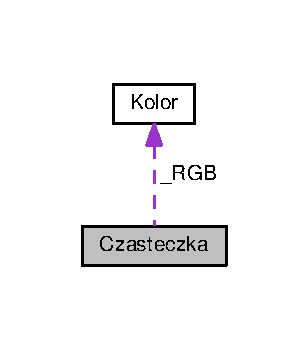
\includegraphics[width=181pt]{class_czasteczka__coll__graph}
\end{center}
\end{figure}
\subsection*{Metody publiczne}
\begin{DoxyCompactItemize}
\item 
\hyperlink{class_czasteczka_a1e73beeb1253fbb91788eabd65bcb0bf}{Czasteczka} (\hyperlink{class_vector}{Vector} \hyperlink{class_czasteczka_a2568977045d9bfe26054029c7657ad17}{xy}, int r, const \hyperlink{class_kolor}{Kolor} \&rgb)
\begin{DoxyCompactList}\small\item\em Konstruktor. \end{DoxyCompactList}\item 
void \hyperlink{class_czasteczka_a3d143798d7b407fe9dff7b61ab2b8071}{Rysuj\-Czasteczke} (Q\-Painter \&Rysownik, const int \hyperlink{class_czasteczka_a1b550be0425165a213fa1cec985b5478}{Promien}, const \hyperlink{class_kolor}{Kolor} \hyperlink{class_czasteczka_a546104013fe302440214f8809d7ec602}{R\-G\-B}, const double x, const double y)
\begin{DoxyCompactList}\small\item\em Metoda rysujaca czasteczke. \end{DoxyCompactList}\item 
\hyperlink{class_vector}{Vector} \hyperlink{class_czasteczka_a2568977045d9bfe26054029c7657ad17}{xy} () const 
\begin{DoxyCompactList}\small\item\em Interfejs pozwalajacy na odczyt prywatnych danych. \end{DoxyCompactList}\item 
\hyperlink{class_vector}{Vector} \& \hyperlink{class_czasteczka_a103b1c45bfeb9d5fec4acf74cd9d53f0}{xy} ()
\begin{DoxyCompactList}\small\item\em Interfejs pozwalajacy na zmiane prywatnych danych. \end{DoxyCompactList}\item 
int \hyperlink{class_czasteczka_a1b550be0425165a213fa1cec985b5478}{Promien} () const 
\begin{DoxyCompactList}\small\item\em Interfejs pozwalajacy na odczyt prywatnych danych. \end{DoxyCompactList}\item 
int \& \hyperlink{class_czasteczka_abd36efdd1f58cdf8a6a8379bfe663f3b}{Promien} ()
\begin{DoxyCompactList}\small\item\em Interfejs pozwalajacy na zmiane prywatnych danych. \end{DoxyCompactList}\item 
\hyperlink{class_kolor}{Kolor} \hyperlink{class_czasteczka_a546104013fe302440214f8809d7ec602}{R\-G\-B} () const 
\begin{DoxyCompactList}\small\item\em Interfejs pozwalajacy na odczyt prywatnych danych. \end{DoxyCompactList}\item 
\hyperlink{class_kolor}{Kolor} \& \hyperlink{class_czasteczka_aa70b19b0f59c5e4b244a9ff203d6de41}{R\-G\-B} ()
\begin{DoxyCompactList}\small\item\em Interfejs pozwalajacy na zmiane prywatnych danych. \end{DoxyCompactList}\end{DoxyCompactItemize}
\subsection*{Atrybuty prywatne}
\begin{DoxyCompactItemize}
\item 
\hyperlink{class_vector}{Vector} \hyperlink{class_czasteczka_a025a3ee895f8ee9c765814cfca1fd5e1}{\-\_\-xy}
\begin{DoxyCompactList}\small\item\em Atrybut opisujacy polozenie czasteczki. \end{DoxyCompactList}\item 
int \hyperlink{class_czasteczka_a5a1d126d89bd571c79a5691c45e2f469}{\-\_\-\-Promien}
\begin{DoxyCompactList}\small\item\em Atrybut okreslajacy promien czasteczki. \end{DoxyCompactList}\item 
\hyperlink{class_kolor}{Kolor} \hyperlink{class_czasteczka_ab9c93cfb3cf0360579ad0def2a94178c}{\-\_\-\-R\-G\-B}
\begin{DoxyCompactList}\small\item\em Atrybut opisujacy kolor czasteczki. \end{DoxyCompactList}\end{DoxyCompactItemize}


\subsection{Opis szczegółowy}
Klasa zawierajaca podstawowe atrybuty czasteczki. 

Definicja w linii 29 pliku czasteczka.\-hh.



\subsection{Dokumentacja konstruktora i destruktora}
\hypertarget{class_czasteczka_a1e73beeb1253fbb91788eabd65bcb0bf}{\index{Czasteczka@{Czasteczka}!Czasteczka@{Czasteczka}}
\index{Czasteczka@{Czasteczka}!Czasteczka@{Czasteczka}}
\subsubsection[{Czasteczka}]{\setlength{\rightskip}{0pt plus 5cm}Czasteczka\-::\-Czasteczka (
\begin{DoxyParamCaption}
\item[{{\bf Vector}}]{xy, }
\item[{int}]{r, }
\item[{const {\bf Kolor} \&}]{rgb}
\end{DoxyParamCaption}
)\hspace{0.3cm}{\ttfamily [inline]}}}\label{class_czasteczka_a1e73beeb1253fbb91788eabd65bcb0bf}
Konstruktor parametryczny, inicjalizujacy czasteczke podanymi wlasnosciami. 
\begin{DoxyParams}[1]{Parametry}
\mbox{\tt in}  & {\em xy} & -\/ wektor polozenia czasteczki \\
\hline
\mbox{\tt in}  & {\em r} & -\/ promien czasteczki \\
\hline
\mbox{\tt in}  & {\em rgb} & -\/ kolor czasteczki \\
\hline
\end{DoxyParams}


Definicja w linii 40 pliku czasteczka.\-hh.



\subsection{Dokumentacja funkcji składowych}
\hypertarget{class_czasteczka_a1b550be0425165a213fa1cec985b5478}{\index{Czasteczka@{Czasteczka}!Promien@{Promien}}
\index{Promien@{Promien}!Czasteczka@{Czasteczka}}
\subsubsection[{Promien}]{\setlength{\rightskip}{0pt plus 5cm}int Czasteczka\-::\-Promien (
\begin{DoxyParamCaption}
{}
\end{DoxyParamCaption}
) const\hspace{0.3cm}{\ttfamily [inline]}}}\label{class_czasteczka_a1b550be0425165a213fa1cec985b5478}
Interfejs pozwalajacy na odczyt prywatnych danych. \begin{DoxyReturn}{Zwraca}
\-\_\-\-Promien -\/ prywatny atrybut opisujacy promien czasteczki 
\end{DoxyReturn}


Definicja w linii 81 pliku czasteczka.\-hh.



Oto graf wywoływań tej funkcji\-:\nopagebreak
\begin{figure}[H]
\begin{center}
\leavevmode
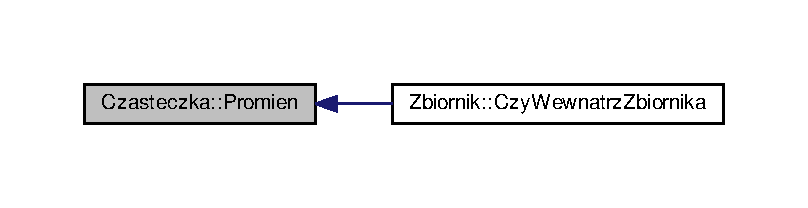
\includegraphics[width=350pt]{class_czasteczka_a1b550be0425165a213fa1cec985b5478_icgraph}
\end{center}
\end{figure}


\hypertarget{class_czasteczka_abd36efdd1f58cdf8a6a8379bfe663f3b}{\index{Czasteczka@{Czasteczka}!Promien@{Promien}}
\index{Promien@{Promien}!Czasteczka@{Czasteczka}}
\subsubsection[{Promien}]{\setlength{\rightskip}{0pt plus 5cm}int\& Czasteczka\-::\-Promien (
\begin{DoxyParamCaption}
{}
\end{DoxyParamCaption}
)\hspace{0.3cm}{\ttfamily [inline]}}}\label{class_czasteczka_abd36efdd1f58cdf8a6a8379bfe663f3b}
Interfejs pozwalajacy na zmiane prywatnych danych. \begin{DoxyReturn}{Zwraca}
\-\_\-\-Promien -\/ referencja na prywatny atrybut opisujacy promien czasteczki 
\end{DoxyReturn}


Definicja w linii 88 pliku czasteczka.\-hh.

\hypertarget{class_czasteczka_a546104013fe302440214f8809d7ec602}{\index{Czasteczka@{Czasteczka}!R\-G\-B@{R\-G\-B}}
\index{R\-G\-B@{R\-G\-B}!Czasteczka@{Czasteczka}}
\subsubsection[{R\-G\-B}]{\setlength{\rightskip}{0pt plus 5cm}{\bf Kolor} Czasteczka\-::\-R\-G\-B (
\begin{DoxyParamCaption}
{}
\end{DoxyParamCaption}
) const\hspace{0.3cm}{\ttfamily [inline]}}}\label{class_czasteczka_a546104013fe302440214f8809d7ec602}
Interfejs pozwalajacy na odczyt prywatnych danych. \begin{DoxyReturn}{Zwraca}
\-\_\-\-R\-G\-B -\/ prywatny atrybut opisujacy polozenie kolor czasteczki 
\end{DoxyReturn}


Definicja w linii 96 pliku czasteczka.\-hh.

\hypertarget{class_czasteczka_aa70b19b0f59c5e4b244a9ff203d6de41}{\index{Czasteczka@{Czasteczka}!R\-G\-B@{R\-G\-B}}
\index{R\-G\-B@{R\-G\-B}!Czasteczka@{Czasteczka}}
\subsubsection[{R\-G\-B}]{\setlength{\rightskip}{0pt plus 5cm}{\bf Kolor}\& Czasteczka\-::\-R\-G\-B (
\begin{DoxyParamCaption}
{}
\end{DoxyParamCaption}
)\hspace{0.3cm}{\ttfamily [inline]}}}\label{class_czasteczka_aa70b19b0f59c5e4b244a9ff203d6de41}
Interfejs pozwalajacy na zmiane prywatnych danych. \begin{DoxyReturn}{Zwraca}
\-\_\-\-R\-G\-B -\/ referencja na prywatny atrybut opisujacy promien czasteczki 
\end{DoxyReturn}


Definicja w linii 103 pliku czasteczka.\-hh.

\hypertarget{class_czasteczka_a3d143798d7b407fe9dff7b61ab2b8071}{\index{Czasteczka@{Czasteczka}!Rysuj\-Czasteczke@{Rysuj\-Czasteczke}}
\index{Rysuj\-Czasteczke@{Rysuj\-Czasteczke}!Czasteczka@{Czasteczka}}
\subsubsection[{Rysuj\-Czasteczke}]{\setlength{\rightskip}{0pt plus 5cm}void Czasteczka\-::\-Rysuj\-Czasteczke (
\begin{DoxyParamCaption}
\item[{Q\-Painter \&}]{Rysownik, }
\item[{const int}]{Promien, }
\item[{const {\bf Kolor}}]{R\-G\-B, }
\item[{const double}]{x, }
\item[{const double}]{y}
\end{DoxyParamCaption}
)}}\label{class_czasteczka_a3d143798d7b407fe9dff7b61ab2b8071}
Rysuje czasteczke o zadanych parametrach 
\begin{DoxyParams}[1]{Parametry}
\mbox{\tt in,out}  & {\em Rysownik} & -\/ referencja na obiekt klasy Q\-Painter \\
\hline
\mbox{\tt in}  & {\em Promien} & -\/ promien czasteczki \\
\hline
\mbox{\tt in}  & {\em R\-G\-B} & -\/ kolor czasteczki w formacie R\-G\-B \\
\hline
\mbox{\tt in}  & {\em x} & -\/ polozenie czasteczki na osi x \\
\hline
\mbox{\tt in}  & {\em y} & -\/ polozenie czasteczki na osi y \\
\hline
\end{DoxyParams}


Definicja w linii 16 pliku czasteczka.\-cpp.



Oto graf wywołań dla tej funkcji\-:\nopagebreak
\begin{figure}[H]
\begin{center}
\leavevmode
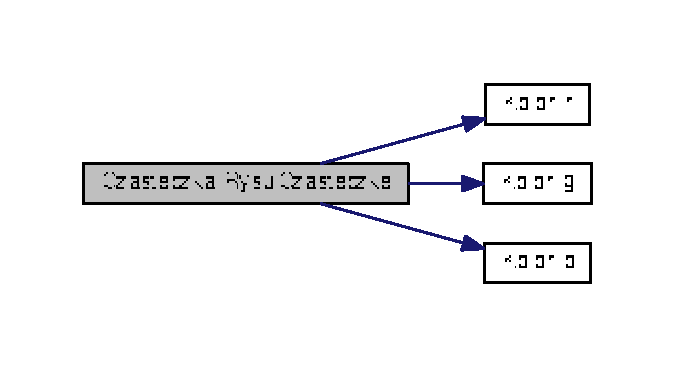
\includegraphics[width=320pt]{class_czasteczka_a3d143798d7b407fe9dff7b61ab2b8071_cgraph}
\end{center}
\end{figure}


\hypertarget{class_czasteczka_a2568977045d9bfe26054029c7657ad17}{\index{Czasteczka@{Czasteczka}!xy@{xy}}
\index{xy@{xy}!Czasteczka@{Czasteczka}}
\subsubsection[{xy}]{\setlength{\rightskip}{0pt plus 5cm}{\bf Vector} Czasteczka\-::xy (
\begin{DoxyParamCaption}
{}
\end{DoxyParamCaption}
) const\hspace{0.3cm}{\ttfamily [inline]}}}\label{class_czasteczka_a2568977045d9bfe26054029c7657ad17}
Interfejs pozwalajacy na odczyt prywatnych danych. \begin{DoxyReturn}{Zwraca}
\-\_\-xy -\/ prywatny atrybut opisujacy polozenie czasteczki 
\end{DoxyReturn}


Definicja w linii 66 pliku czasteczka.\-hh.



Oto graf wywoływań tej funkcji\-:\nopagebreak
\begin{figure}[H]
\begin{center}
\leavevmode
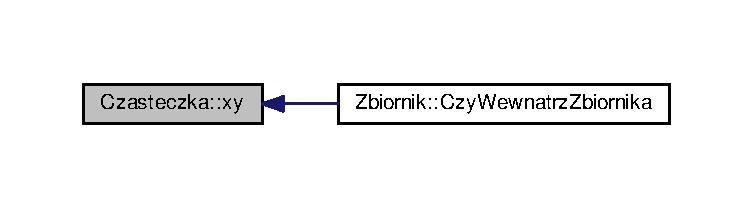
\includegraphics[width=350pt]{class_czasteczka_a2568977045d9bfe26054029c7657ad17_icgraph}
\end{center}
\end{figure}


\hypertarget{class_czasteczka_a103b1c45bfeb9d5fec4acf74cd9d53f0}{\index{Czasteczka@{Czasteczka}!xy@{xy}}
\index{xy@{xy}!Czasteczka@{Czasteczka}}
\subsubsection[{xy}]{\setlength{\rightskip}{0pt plus 5cm}{\bf Vector}\& Czasteczka\-::xy (
\begin{DoxyParamCaption}
{}
\end{DoxyParamCaption}
)\hspace{0.3cm}{\ttfamily [inline]}}}\label{class_czasteczka_a103b1c45bfeb9d5fec4acf74cd9d53f0}
Interfejs pozwalajacy na zmiane prywatnych danych. \begin{DoxyReturn}{Zwraca}
\-\_\-xy -\/ referencja na prywatny atrybut opisujacy polozenie czasteczki 
\end{DoxyReturn}


Definicja w linii 73 pliku czasteczka.\-hh.



\subsection{Dokumentacja atrybutów składowych}
\hypertarget{class_czasteczka_a5a1d126d89bd571c79a5691c45e2f469}{\index{Czasteczka@{Czasteczka}!\-\_\-\-Promien@{\-\_\-\-Promien}}
\index{\-\_\-\-Promien@{\-\_\-\-Promien}!Czasteczka@{Czasteczka}}
\subsubsection[{\-\_\-\-Promien}]{\setlength{\rightskip}{0pt plus 5cm}int Czasteczka\-::\-\_\-\-Promien\hspace{0.3cm}{\ttfamily [private]}}}\label{class_czasteczka_a5a1d126d89bd571c79a5691c45e2f469}
Atrybut okreslajacy promien czasteczki. 

Definicja w linii 118 pliku czasteczka.\-hh.

\hypertarget{class_czasteczka_ab9c93cfb3cf0360579ad0def2a94178c}{\index{Czasteczka@{Czasteczka}!\-\_\-\-R\-G\-B@{\-\_\-\-R\-G\-B}}
\index{\-\_\-\-R\-G\-B@{\-\_\-\-R\-G\-B}!Czasteczka@{Czasteczka}}
\subsubsection[{\-\_\-\-R\-G\-B}]{\setlength{\rightskip}{0pt plus 5cm}{\bf Kolor} Czasteczka\-::\-\_\-\-R\-G\-B\hspace{0.3cm}{\ttfamily [private]}}}\label{class_czasteczka_ab9c93cfb3cf0360579ad0def2a94178c}
Atrybut opisujacy kolor czasteczki. 

Definicja w linii 125 pliku czasteczka.\-hh.

\hypertarget{class_czasteczka_a025a3ee895f8ee9c765814cfca1fd5e1}{\index{Czasteczka@{Czasteczka}!\-\_\-xy@{\-\_\-xy}}
\index{\-\_\-xy@{\-\_\-xy}!Czasteczka@{Czasteczka}}
\subsubsection[{\-\_\-xy}]{\setlength{\rightskip}{0pt plus 5cm}{\bf Vector} Czasteczka\-::\-\_\-xy\hspace{0.3cm}{\ttfamily [private]}}}\label{class_czasteczka_a025a3ee895f8ee9c765814cfca1fd5e1}
Atrybut opisujacy polozenie czasteczki w kartezjanskim ukladzie wspolrzednych. 

Definicja w linii 103 pliku czasteczka.\-hh.



Dokumentacja dla tej klasy została wygenerowana z plików\-:\begin{DoxyCompactItemize}
\item 
\hyperlink{czasteczka_8hh}{czasteczka.\-hh}\item 
\hyperlink{czasteczka_8cpp}{czasteczka.\-cpp}\end{DoxyCompactItemize}

\hypertarget{class_ui_1_1_d_main_window}{\section{Dokumentacja klasy Ui\-:\-:D\-Main\-Window}
\label{class_ui_1_1_d_main_window}\index{Ui\-::\-D\-Main\-Window@{Ui\-::\-D\-Main\-Window}}
}


{\ttfamily \#include $<$ui\-\_\-dmainwindow.\-h$>$}



Diagram dziedziczenia dla Ui\-:\-:D\-Main\-Window
\nopagebreak
\begin{figure}[H]
\begin{center}
\leavevmode
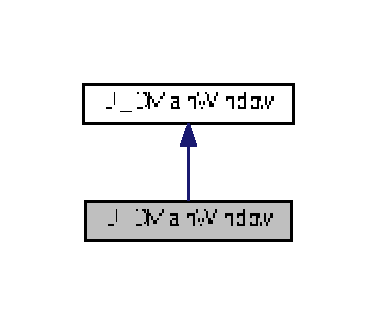
\includegraphics[width=176pt]{class_ui_1_1_d_main_window__inherit__graph}
\end{center}
\end{figure}


Diagram współpracy dla Ui\-:\-:D\-Main\-Window\-:
\nopagebreak
\begin{figure}[H]
\begin{center}
\leavevmode
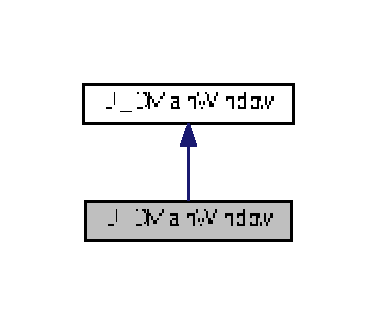
\includegraphics[width=176pt]{class_ui_1_1_d_main_window__coll__graph}
\end{center}
\end{figure}
\subsection*{Dodatkowe Dziedziczone Składowe}


\subsection{Opis szczegółowy}


Definicja w linii 138 pliku ui\-\_\-dmainwindow.\-h.



Dokumentacja dla tej klasy została wygenerowana z pliku\-:\begin{DoxyCompactItemize}
\item 
\hyperlink{ui__dmainwindow_8h}{ui\-\_\-dmainwindow.\-h}\end{DoxyCompactItemize}

\hypertarget{class_kolor}{}\section{Dokumentacja klasy Kolor}
\label{class_kolor}\index{Kolor@{Kolor}}


Klasa modelująca kolor.  




{\ttfamily \#include $<$kolor.\+hh$>$}

\subsection*{Metody publiczne}
\begin{DoxyCompactItemize}
\item 
\hyperlink{class_kolor_adde4f304856649a8a148288c271d4775}{Kolor} (int \hyperlink{class_kolor_a1091fbdb6e53516bfb68784e96e58bc1}{r}, int \hyperlink{class_kolor_a4dfa47458440fb136711fb6de6344f61}{g}, int \hyperlink{class_kolor_aa240903064a3d8f49585c34d92b74e5d}{b})
\begin{DoxyCompactList}\small\item\em Konstruktor. \end{DoxyCompactList}\item 
\hyperlink{class_kolor_a79baff3add17cc61abb8bc71f0a426e6}{Kolor} (const \hyperlink{class_kolor}{Kolor} \&rgb)
\begin{DoxyCompactList}\small\item\em Konstruktor kopiujacy. \end{DoxyCompactList}\item 
int \hyperlink{class_kolor_a1091fbdb6e53516bfb68784e96e58bc1}{r} () const 
\begin{DoxyCompactList}\small\item\em Interfejs pozwalajacy na odczyt prywatnych danych. \end{DoxyCompactList}\item 
int \& \hyperlink{class_kolor_a426240b4b7c4364e9d34db265475b4ad}{r} ()
\begin{DoxyCompactList}\small\item\em Interfejs pozwalajacy na zmiane prywatnych danych. \end{DoxyCompactList}\item 
int \hyperlink{class_kolor_a4dfa47458440fb136711fb6de6344f61}{g} () const 
\begin{DoxyCompactList}\small\item\em Interfejs pozwalajacy na odczyt prywatnych danych. \end{DoxyCompactList}\item 
int \& \hyperlink{class_kolor_ab5e20d58c58d42747c16155a83aa906f}{g} ()
\begin{DoxyCompactList}\small\item\em Interfejs pozwalajacy na zmiane prywatnych danych. \end{DoxyCompactList}\item 
int \hyperlink{class_kolor_aa240903064a3d8f49585c34d92b74e5d}{b} () const 
\begin{DoxyCompactList}\small\item\em Interfejs pozwalajacy na odczyt prywatnych danych. \end{DoxyCompactList}\item 
int \& \hyperlink{class_kolor_a87677bdafb912de9526302f4844f86a7}{b} ()
\begin{DoxyCompactList}\small\item\em Interfejs pozwalajacy na zmiane prywatnych danych. \end{DoxyCompactList}\end{DoxyCompactItemize}
\subsection*{Atrybuty prywatne}
\begin{DoxyCompactItemize}
\item 
int \hyperlink{class_kolor_ad887fb53be523b39fbead6a24671751e}{\+\_\+r}
\begin{DoxyCompactList}\small\item\em Atrybut opisujacy wartosc odcieniu czerwonego. \end{DoxyCompactList}\item 
int \hyperlink{class_kolor_a568f73268d43f0e76c8ae75f0ef20229}{\+\_\+g}
\begin{DoxyCompactList}\small\item\em Atrybut opisujacy wartosc odcieniu zielonego. \end{DoxyCompactList}\item 
int \hyperlink{class_kolor_a543b5984743ac9d471409c697382038b}{\+\_\+b}
\begin{DoxyCompactList}\small\item\em Atrybut opisujacy wartosc odcieniu niebieskiego. \end{DoxyCompactList}\end{DoxyCompactItemize}


\subsection{Opis szczegółowy}
Klasa opisuje kolor w formacie R\+G\+B. Każdy z kolorów przyjmuje wartości z zakresu \mbox{[}0, 255\mbox{]}. 

Definicja w linii 25 pliku kolor.\+hh.



\subsection{Dokumentacja konstruktora i destruktora}
\hypertarget{class_kolor_adde4f304856649a8a148288c271d4775}{}\index{Kolor@{Kolor}!Kolor@{Kolor}}
\index{Kolor@{Kolor}!Kolor@{Kolor}}
\subsubsection[{Kolor}]{\setlength{\rightskip}{0pt plus 5cm}Kolor\+::\+Kolor (
\begin{DoxyParamCaption}
\item[{int}]{r, }
\item[{int}]{g, }
\item[{int}]{b}
\end{DoxyParamCaption}
)\hspace{0.3cm}{\ttfamily [inline]}}\label{class_kolor_adde4f304856649a8a148288c271d4775}
Konstruktor parametryczny, inicjalizujacy kolor podanymi wartosciami. 
\begin{DoxyParams}[1]{Parametry}
\mbox{\tt in}  & {\em r} & -\/ wartosc odcieniu czerwonego, \mbox{[}0, 255\mbox{]} \\
\hline
\mbox{\tt in}  & {\em g} & -\/ wartosc odcieniu zielonego, \mbox{[}0, 255\mbox{]} \\
\hline
\mbox{\tt in}  & {\em b} & -\/ wartosc odcieniu niebieskiego, \mbox{[}0, 255\mbox{]} \\
\hline
\end{DoxyParams}


Definicja w linii 36 pliku kolor.\+hh.



Oto graf wywołań dla tej funkcji\+:\nopagebreak
\begin{figure}[H]
\begin{center}
\leavevmode
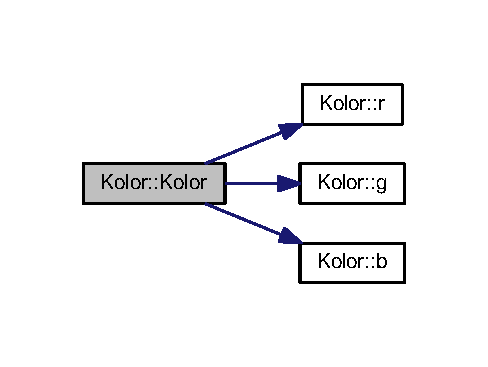
\includegraphics[width=239pt]{class_kolor_adde4f304856649a8a148288c271d4775_cgraph}
\end{center}
\end{figure}


\hypertarget{class_kolor_a79baff3add17cc61abb8bc71f0a426e6}{}\index{Kolor@{Kolor}!Kolor@{Kolor}}
\index{Kolor@{Kolor}!Kolor@{Kolor}}
\subsubsection[{Kolor}]{\setlength{\rightskip}{0pt plus 5cm}Kolor\+::\+Kolor (
\begin{DoxyParamCaption}
\item[{const {\bf Kolor} \&}]{rgb}
\end{DoxyParamCaption}
)\hspace{0.3cm}{\ttfamily [inline]}}\label{class_kolor_a79baff3add17cc61abb8bc71f0a426e6}
Konstruktor kopiujacy. 
\begin{DoxyParams}[1]{Parametry}
\mbox{\tt in}  & {\em rgb} & -\/ obiekt do skopiowania \\
\hline
\end{DoxyParams}


Definicja w linii 44 pliku kolor.\+hh.



\subsection{Dokumentacja funkcji składowych}
\hypertarget{class_kolor_aa240903064a3d8f49585c34d92b74e5d}{}\index{Kolor@{Kolor}!b@{b}}
\index{b@{b}!Kolor@{Kolor}}
\subsubsection[{b}]{\setlength{\rightskip}{0pt plus 5cm}int Kolor\+::b (
\begin{DoxyParamCaption}
{}
\end{DoxyParamCaption}
) const\hspace{0.3cm}{\ttfamily [inline]}}\label{class_kolor_aa240903064a3d8f49585c34d92b74e5d}
Interfejs pozwalajacy na odczyt prywatnych danych. \begin{DoxyReturn}{Zwraca}
\+\_\+b -\/ prywatny atrybut opisujacy niebieski odcien 
\end{DoxyReturn}


Definicja w linii 82 pliku kolor.\+hh.



Oto graf wywoływań tej funkcji\+:\nopagebreak
\begin{figure}[H]
\begin{center}
\leavevmode
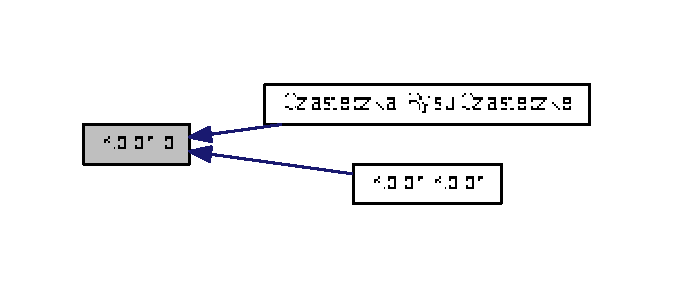
\includegraphics[width=323pt]{class_kolor_aa240903064a3d8f49585c34d92b74e5d_icgraph}
\end{center}
\end{figure}


\hypertarget{class_kolor_a87677bdafb912de9526302f4844f86a7}{}\index{Kolor@{Kolor}!b@{b}}
\index{b@{b}!Kolor@{Kolor}}
\subsubsection[{b}]{\setlength{\rightskip}{0pt plus 5cm}int\& Kolor\+::b (
\begin{DoxyParamCaption}
{}
\end{DoxyParamCaption}
)\hspace{0.3cm}{\ttfamily [inline]}}\label{class_kolor_a87677bdafb912de9526302f4844f86a7}
Interfejs pozwalajacy na zmiane prywatnych danych. \begin{DoxyReturn}{Zwraca}
\+\_\+b -\/ referencja na prywatny atrybut opisujacy niebieski odcien 
\end{DoxyReturn}


Definicja w linii 89 pliku kolor.\+hh.

\hypertarget{class_kolor_a4dfa47458440fb136711fb6de6344f61}{}\index{Kolor@{Kolor}!g@{g}}
\index{g@{g}!Kolor@{Kolor}}
\subsubsection[{g}]{\setlength{\rightskip}{0pt plus 5cm}int Kolor\+::g (
\begin{DoxyParamCaption}
{}
\end{DoxyParamCaption}
) const\hspace{0.3cm}{\ttfamily [inline]}}\label{class_kolor_a4dfa47458440fb136711fb6de6344f61}
Interfejs pozwalajacy na odczyt prywatnych danych. \begin{DoxyReturn}{Zwraca}
\+\_\+g -\/ prywatny atrybut opisujacy zielony odcien 
\end{DoxyReturn}


Definicja w linii 67 pliku kolor.\+hh.



Oto graf wywoływań tej funkcji\+:\nopagebreak
\begin{figure}[H]
\begin{center}
\leavevmode
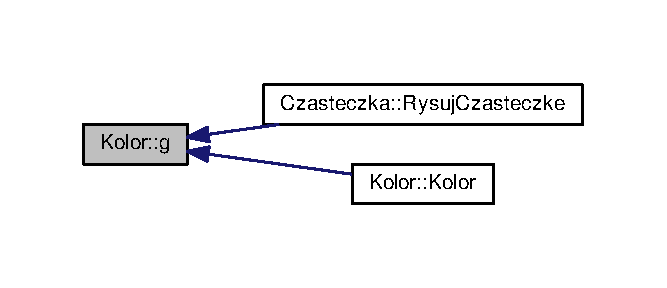
\includegraphics[width=324pt]{class_kolor_a4dfa47458440fb136711fb6de6344f61_icgraph}
\end{center}
\end{figure}


\hypertarget{class_kolor_ab5e20d58c58d42747c16155a83aa906f}{}\index{Kolor@{Kolor}!g@{g}}
\index{g@{g}!Kolor@{Kolor}}
\subsubsection[{g}]{\setlength{\rightskip}{0pt plus 5cm}int\& Kolor\+::g (
\begin{DoxyParamCaption}
{}
\end{DoxyParamCaption}
)\hspace{0.3cm}{\ttfamily [inline]}}\label{class_kolor_ab5e20d58c58d42747c16155a83aa906f}
Interfejs pozwalajacy na zmiane prywatnych danych. \begin{DoxyReturn}{Zwraca}
\+\_\+g -\/ referencja na prywatny atrybut opisujacy zielony odcien 
\end{DoxyReturn}


Definicja w linii 74 pliku kolor.\+hh.

\hypertarget{class_kolor_a1091fbdb6e53516bfb68784e96e58bc1}{}\index{Kolor@{Kolor}!r@{r}}
\index{r@{r}!Kolor@{Kolor}}
\subsubsection[{r}]{\setlength{\rightskip}{0pt plus 5cm}int Kolor\+::r (
\begin{DoxyParamCaption}
{}
\end{DoxyParamCaption}
) const\hspace{0.3cm}{\ttfamily [inline]}}\label{class_kolor_a1091fbdb6e53516bfb68784e96e58bc1}
Interfejs pozwalajacy na odczyt prywatnych danych. \begin{DoxyReturn}{Zwraca}
\+\_\+r -\/ prywatny atrybut opisujacy czerwony odcien 
\end{DoxyReturn}


Definicja w linii 52 pliku kolor.\+hh.



Oto graf wywoływań tej funkcji\+:\nopagebreak
\begin{figure}[H]
\begin{center}
\leavevmode
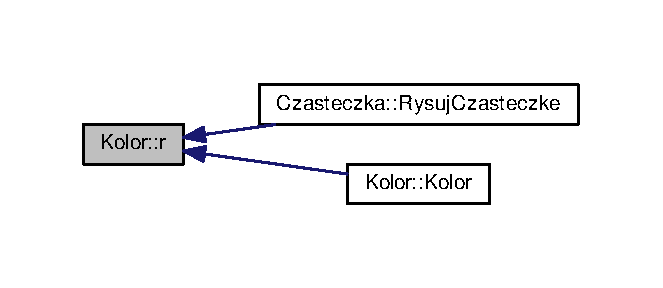
\includegraphics[width=322pt]{class_kolor_a1091fbdb6e53516bfb68784e96e58bc1_icgraph}
\end{center}
\end{figure}


\hypertarget{class_kolor_a426240b4b7c4364e9d34db265475b4ad}{}\index{Kolor@{Kolor}!r@{r}}
\index{r@{r}!Kolor@{Kolor}}
\subsubsection[{r}]{\setlength{\rightskip}{0pt plus 5cm}int\& Kolor\+::r (
\begin{DoxyParamCaption}
{}
\end{DoxyParamCaption}
)\hspace{0.3cm}{\ttfamily [inline]}}\label{class_kolor_a426240b4b7c4364e9d34db265475b4ad}
Interfejs pozwalajacy na zmiane prywatnych danych. \begin{DoxyReturn}{Zwraca}
\+\_\+r -\/ referencja na prywatny atrybut opisujacy czerwony odcien 
\end{DoxyReturn}


Definicja w linii 59 pliku kolor.\+hh.



\subsection{Dokumentacja atrybutów składowych}
\hypertarget{class_kolor_a543b5984743ac9d471409c697382038b}{}\index{Kolor@{Kolor}!\+\_\+b@{\+\_\+b}}
\index{\+\_\+b@{\+\_\+b}!Kolor@{Kolor}}
\subsubsection[{\+\_\+b}]{\setlength{\rightskip}{0pt plus 5cm}int Kolor\+::\+\_\+b\hspace{0.3cm}{\ttfamily [private]}}\label{class_kolor_a543b5984743ac9d471409c697382038b}
Atrybut opisujacy wartosc odcieniu niebieskiego. 

Definicja w linii 111 pliku kolor.\+hh.

\hypertarget{class_kolor_a568f73268d43f0e76c8ae75f0ef20229}{}\index{Kolor@{Kolor}!\+\_\+g@{\+\_\+g}}
\index{\+\_\+g@{\+\_\+g}!Kolor@{Kolor}}
\subsubsection[{\+\_\+g}]{\setlength{\rightskip}{0pt plus 5cm}int Kolor\+::\+\_\+g\hspace{0.3cm}{\ttfamily [private]}}\label{class_kolor_a568f73268d43f0e76c8ae75f0ef20229}
Atrybut opisujacy wartosc odcieniu zielonego. 

Definicja w linii 104 pliku kolor.\+hh.

\hypertarget{class_kolor_ad887fb53be523b39fbead6a24671751e}{}\index{Kolor@{Kolor}!\+\_\+r@{\+\_\+r}}
\index{\+\_\+r@{\+\_\+r}!Kolor@{Kolor}}
\subsubsection[{\+\_\+r}]{\setlength{\rightskip}{0pt plus 5cm}int Kolor\+::\+\_\+r\hspace{0.3cm}{\ttfamily [private]}}\label{class_kolor_ad887fb53be523b39fbead6a24671751e}
Atrybut opisujacy wartosc odcieniu czerwonego. 

Definicja w linii 89 pliku kolor.\+hh.



Dokumentacja dla tej klasy została wygenerowana z pliku\+:\begin{DoxyCompactItemize}
\item 
\hyperlink{kolor_8hh}{kolor.\+hh}\end{DoxyCompactItemize}

\hypertarget{class_okno_glowne}{\section{Dokumentacja klasy Okno\-Glowne}
\label{class_okno_glowne}\index{Okno\-Glowne@{Okno\-Glowne}}
}


Klasa modelujaca głowne okno aplikacji.  




{\ttfamily \#include $<$okno\-\_\-glowne.\-hh$>$}



Diagram dziedziczenia dla Okno\-Glowne\nopagebreak
\begin{figure}[H]
\begin{center}
\leavevmode
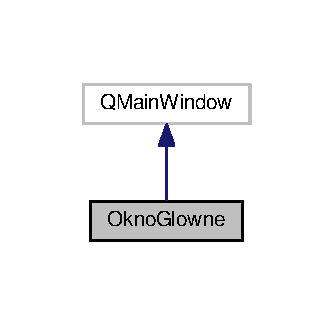
\includegraphics[width=160pt]{class_okno_glowne__inherit__graph}
\end{center}
\end{figure}


Diagram współpracy dla Okno\-Glowne\-:\nopagebreak
\begin{figure}[H]
\begin{center}
\leavevmode
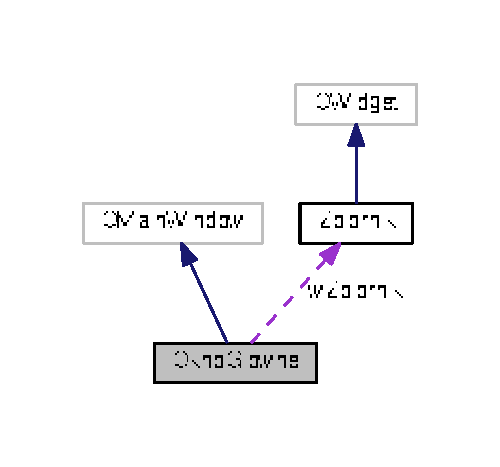
\includegraphics[width=293pt]{class_okno_glowne__coll__graph}
\end{center}
\end{figure}
\subsection*{Sloty publiczne}
\begin{DoxyCompactItemize}
\item 
void \hyperlink{class_okno_glowne_a2a49d3696ef8a42325313842768f2c92}{Gdy\-Odpowiedni\-Czas} ()
\begin{DoxyCompactList}\small\item\em Slot odpowiadajacy za aktualizacje danych. . \end{DoxyCompactList}\item 
void \hyperlink{class_okno_glowne_a2a59f13292adfead4ac821780220044a}{Gdy\-Napis} (const Q\-String \&)
\begin{DoxyCompactList}\small\item\em Slot odpowiadajacy za wyswietlenie napisu po otrzymaniu sygnalu. \end{DoxyCompactList}\item 
void \hyperlink{class_okno_glowne_ac837b1f8c8b0288d07987e059966431b}{on\-\_\-play\-Button\-\_\-clicked} ()
\begin{DoxyCompactList}\small\item\em Slot odpowiadajacy za obsluge stanu play. \end{DoxyCompactList}\item 
void \hyperlink{class_okno_glowne_ae8bd560de9aa835ba8b194b8f7da094c}{on\-\_\-pause\-Button\-\_\-clicked} ()
\begin{DoxyCompactList}\small\item\em Slot odpowiadajacy za obsluge stanu pauza. \end{DoxyCompactList}\item 
void \hyperlink{class_okno_glowne_a63255adc6263a1ee6f67c96b91446b73}{on\-\_\-stop\-Button\-\_\-clicked} ()
\begin{DoxyCompactList}\small\item\em Slot odpowiadajacy za obsluge stanu stop. \end{DoxyCompactList}\item 
void \hyperlink{class_okno_glowne_aba5accbf5e231ba194ee0e966b8d7b15}{on\-\_\-load\-Button\-\_\-clicked} ()
\begin{DoxyCompactList}\small\item\em Slot odpowiadajacy za wczytanie danych z pliku. \end{DoxyCompactList}\item 
void \hyperlink{class_okno_glowne_a0c744f19fcf0e4bcd04a49502864e020}{on\-\_\-line\-Edit\-\_\-return\-Pressed} ()
\begin{DoxyCompactList}\small\item\em Slot odpowiadajacy za wczytanie danych z pliku. \end{DoxyCompactList}\item 
void \hyperlink{class_okno_glowne_a726ce3fbe89c3fb7364c39e99c0ad658}{on\-\_\-slider\-Szybkosc\-Sym\-\_\-value\-Changed} (int a)
\begin{DoxyCompactList}\small\item\em Slot odpowiadajacy za zmiane wartosci slidera. \end{DoxyCompactList}\item 
void \hyperlink{class_okno_glowne_a8ed8fc49c9c3d3e187639880ce286c88}{on\-\_\-action\-\_\-\-Save\-\_\-triggered} ()
\begin{DoxyCompactList}\small\item\em Slot odpowiadajacy za przycisniecie przycisku Save. \end{DoxyCompactList}\end{DoxyCompactItemize}
\subsection*{Sygnały}
\begin{DoxyCompactItemize}
\item 
void \hyperlink{class_okno_glowne_aa602a0c5a940f0af4ab7390bfc1a4b9d}{Zglos\-Napis} (const Q\-String \&)
\begin{DoxyCompactList}\small\item\em Sygnal zglaszajacy napis. \end{DoxyCompactList}\end{DoxyCompactItemize}
\subsection*{Metody publiczne}
\begin{DoxyCompactItemize}
\item 
\hyperlink{class_okno_glowne_a8dcfe4e0f18dfaf0c535c4549991b550}{Okno\-Glowne} (Q\-Widget $\ast$w\-Rodzic=N\-U\-L\-L)
\begin{DoxyCompactList}\small\item\em Konstruktor. \end{DoxyCompactList}\item 
virtual void \hyperlink{class_okno_glowne_a570c795e3829c3bd7896551c0624abe2}{paint\-Event} (Q\-Paint\-Event $\ast$event)
\begin{DoxyCompactList}\small\item\em Wirtualna metoda paint\-Event wyrysowujaca obiekty na ekranie. \end{DoxyCompactList}\item 
void \hyperlink{class_okno_glowne_a6062f76fdf15ad8bc0543cfd2a2fe150}{Zapisz\-Symulacje\-Do\-Pliku} ()
\begin{DoxyCompactList}\small\item\em Metoda zapisujaca aktualny stan symulacji do pliku. \end{DoxyCompactList}\item 
void \hyperlink{class_okno_glowne_a1b8098c27e9656235bb056aeb79a8ece}{Wczytaj\-Symulacje\-Z\-Pliku} (const std\-::string nazwa\-\_\-pliku)
\begin{DoxyCompactList}\small\item\em Metoda wczytujaca z pliku stan symulacji. \end{DoxyCompactList}\end{DoxyCompactItemize}
\subsection*{Atrybuty publiczne}
\begin{DoxyCompactItemize}
\item 
Q\-Timer \hyperlink{class_okno_glowne_a5d047f90666212f58e69d11af3285d9b}{\-\_\-\-Stoper}
\begin{DoxyCompactList}\small\item\em Miernik czasu. \end{DoxyCompactList}\end{DoxyCompactItemize}
\subsection*{Atrybuty prywatne}
\begin{DoxyCompactItemize}
\item 
\hyperlink{class_zbiornik}{Zbiornik} $\ast$ \hyperlink{class_okno_glowne_af2d1275209898ebdd5ab9de8ef78dffd}{w\-Zbiornik}
\begin{DoxyCompactList}\small\item\em Wskaznik na zbiornik. \end{DoxyCompactList}\item 
Q\-Menu\-Bar $\ast$ \hyperlink{class_okno_glowne_a5a87098d9d4bd868670f5a5e72023a0a}{menu\-Bar}
\begin{DoxyCompactList}\small\item\em Wskaznik na pasek menu. \end{DoxyCompactList}\item 
Q\-Action $\ast$ \hyperlink{class_okno_glowne_a2c2d825b6e5e0faa5eb368be4fc73b78}{action\-\_\-\-Save}
\begin{DoxyCompactList}\small\item\em Wskaznik na akcje przycisku menu Save. \end{DoxyCompactList}\item 
Q\-Action $\ast$ \hyperlink{class_okno_glowne_a579ef9901f57057368cb522ea5a9a5c3}{action\-\_\-\-Exit}
\begin{DoxyCompactList}\small\item\em Wskaznik na akcje przycisku menu Exit. \end{DoxyCompactList}\item 
Q\-Menu $\ast$ \hyperlink{class_okno_glowne_a1ba162db2d0b06b0f8963e61b3806875}{menu\-\_\-\-File}
\begin{DoxyCompactList}\small\item\em Wskaznik na akcje przycisku menu File. \end{DoxyCompactList}\item 
Q\-Menu $\ast$ \hyperlink{class_okno_glowne_a93afadd0ec22ce6a7e29acc5dd2423a2}{menu\-\_\-\-Edit}
\begin{DoxyCompactList}\small\item\em Wskaznik na akcje przycisku menu Edit. \end{DoxyCompactList}\item 
Q\-Menu $\ast$ \hyperlink{class_okno_glowne_ab17be6714913af0cdf4e7de7cb6210d1}{menu\-\_\-\-Help}
\begin{DoxyCompactList}\small\item\em Wskaznik na akcje przycisku menu Help. \end{DoxyCompactList}\item 
Q\-Status\-Bar $\ast$ \hyperlink{class_okno_glowne_a40a10989bc6b318ac24e2457d7adb53b}{status\-Bar}
\begin{DoxyCompactList}\small\item\em Wskaznik na pasek statusowy. \end{DoxyCompactList}\item 
Q\-Tool\-Bar $\ast$ \hyperlink{class_okno_glowne_a6a37dd1f32605092fff7feac712bf429}{tool\-Bar}
\begin{DoxyCompactList}\small\item\em Wskaznik na pasek narzedziowy. \end{DoxyCompactList}\item 
Q\-H\-Box\-Layout $\ast$ \hyperlink{class_okno_glowne_aacb5ddb6d0eb560a47917cc1b457239a}{horizontal\-Layout}
\begin{DoxyCompactList}\small\item\em Wskaznik na obszar do horyzontalnego rozmieszczenia przyciskow. \end{DoxyCompactList}\item 
Q\-Widget $\ast$ \hyperlink{class_okno_glowne_a12ac2d00b9ca186176ccc710a928a723}{horizontal\-Layout\-Widget}
\begin{DoxyCompactList}\small\item\em Wskaznik na widget odpowiedzialny za horyzontalne wyswietlenie przyciskow. \end{DoxyCompactList}\item 
Q\-Push\-Button $\ast$ \hyperlink{class_okno_glowne_a50f936486c1bc3b3278823a8eb90841e}{play\-Button}
\begin{DoxyCompactList}\small\item\em Wskaznik na przycisk play. \end{DoxyCompactList}\item 
Q\-Push\-Button $\ast$ \hyperlink{class_okno_glowne_a0dde8df8a49b8f47f17f8e748fd15967}{pause\-Button}
\begin{DoxyCompactList}\small\item\em Wskaznik na przycisk pause. \end{DoxyCompactList}\item 
Q\-Push\-Button $\ast$ \hyperlink{class_okno_glowne_a3051d73dc0e0a27dc30ada43cc6b63c4}{stop\-Button}
\begin{DoxyCompactList}\small\item\em Wskaznik na przycisk stop. \end{DoxyCompactList}\item 
Q\-Push\-Button $\ast$ \hyperlink{class_okno_glowne_accbadc3bc4d418cfe1bce2be61881917}{load\-Button}
\begin{DoxyCompactList}\small\item\em Wskaznik na przycisk Wczytaj. \end{DoxyCompactList}\item 
Q\-Slider $\ast$ \hyperlink{class_okno_glowne_a85328893065393400d5a0344004ca78b}{slider\-Szybkosc\-Sym}
\begin{DoxyCompactList}\small\item\em Wskaznik na slider. \end{DoxyCompactList}\item 
Q\-L\-C\-D\-Number $\ast$ \hyperlink{class_okno_glowne_ab100c00d4ba33d896fd0985ac366296a}{lcd\-Szybkosc\-Sym}
\begin{DoxyCompactList}\small\item\em Wskaznik na L\-C\-D z szybkoscia symulacji. \end{DoxyCompactList}\item 
Q\-Label $\ast$ \hyperlink{class_okno_glowne_ad7b0708ffdf61f3bef1349cc353a6c4e}{label\-Szybkosc\-Sym}
\begin{DoxyCompactList}\small\item\em Wskaznik na etykiete z szybkoscia symulacji. \end{DoxyCompactList}\item 
Q\-Label $\ast$ \hyperlink{class_okno_glowne_aca07e1dc5cbe30d6952f9b952073bb79}{label\-Czas\-Sym}
\begin{DoxyCompactList}\small\item\em Wskaznik na etykiete z czasem symulacji. \end{DoxyCompactList}\item 
Q\-L\-C\-D\-Number $\ast$ \hyperlink{class_okno_glowne_ab34fefe738e38b1b0d4ce764481cc0c6}{lcd\-Czas\-Sym}
\begin{DoxyCompactList}\small\item\em Wskaznik na L\-C\-D z czasem trwania symulacji. \end{DoxyCompactList}\item 
Q\-Label $\ast$ \hyperlink{class_okno_glowne_ab01460f1222d0ec2892abf21efb23078}{label\-Liczba\-Czasteczek}
\begin{DoxyCompactList}\small\item\em Wskaznik na etykiete z liczbe czasteczek. \end{DoxyCompactList}\item 
Q\-L\-C\-D\-Number $\ast$ \hyperlink{class_okno_glowne_adbdd9fc009725804e015d267dc8375dc}{lcd\-Liczba\-Czasteczek}
\begin{DoxyCompactList}\small\item\em Wskaznik na L\-C\-D z liczbe czasteczek. \end{DoxyCompactList}\item 
Q\-Line\-Edit $\ast$ \hyperlink{class_okno_glowne_a0112b8be70a26552b03f38fab43a3301}{line\-Edit}
\begin{DoxyCompactList}\small\item\em Wskaznik na linijke do wpisywania tekstu. \end{DoxyCompactList}\item 
double \hyperlink{class_okno_glowne_a6a0922607c0970ecdfe8adec7a773c7f}{\-\_\-old\-\_\-width}
\begin{DoxyCompactList}\small\item\em Stara szerokosc okienka. \end{DoxyCompactList}\item 
double \hyperlink{class_okno_glowne_a7dae1b25dbade179eb6dfc30ffeab14b}{\-\_\-old\-\_\-height}
\begin{DoxyCompactList}\small\item\em Stara wysokosc okienka. \end{DoxyCompactList}\end{DoxyCompactItemize}
\subsection*{Statyczne atrybuty prywatne}
\begin{DoxyCompactItemize}
\item 
static int \hyperlink{class_okno_glowne_ae615cbd9c9f9ab06b365c4692ff68729}{licznik\-\_\-plikow}
\begin{DoxyCompactList}\small\item\em Sluzy do generowania unikatowych nazw plikow wyjsciowych. \end{DoxyCompactList}\end{DoxyCompactItemize}


\subsection{Opis szczegółowy}
Dzieki tej klasie wyswietlane jest okno glowne aplikacji. 

Definicja w linii 68 pliku okno\-\_\-glowne.\-hh.



\subsection{Dokumentacja konstruktora i destruktora}
\hypertarget{class_okno_glowne_a8dcfe4e0f18dfaf0c535c4549991b550}{\index{Okno\-Glowne@{Okno\-Glowne}!Okno\-Glowne@{Okno\-Glowne}}
\index{Okno\-Glowne@{Okno\-Glowne}!OknoGlowne@{Okno\-Glowne}}
\subsubsection[{Okno\-Glowne}]{\setlength{\rightskip}{0pt plus 5cm}Okno\-Glowne\-::\-Okno\-Glowne (
\begin{DoxyParamCaption}
\item[{Q\-Widget $\ast$}]{w\-Rodzic = {\ttfamily NULL}}
\end{DoxyParamCaption}
)}}\label{class_okno_glowne_a8dcfe4e0f18dfaf0c535c4549991b550}
Konstruktor parametryczny. 
\begin{DoxyParams}[1]{Parametry}
\mbox{\tt in,out}  & {\em w\-Rodzic} & -\/ wskaznik na rodzica \\
\hline
\end{DoxyParams}


Definicja w linii 16 pliku okno\-\_\-glowne.\-cpp.



Oto graf wywołań dla tej funkcji\-:\nopagebreak
\begin{figure}[H]
\begin{center}
\leavevmode
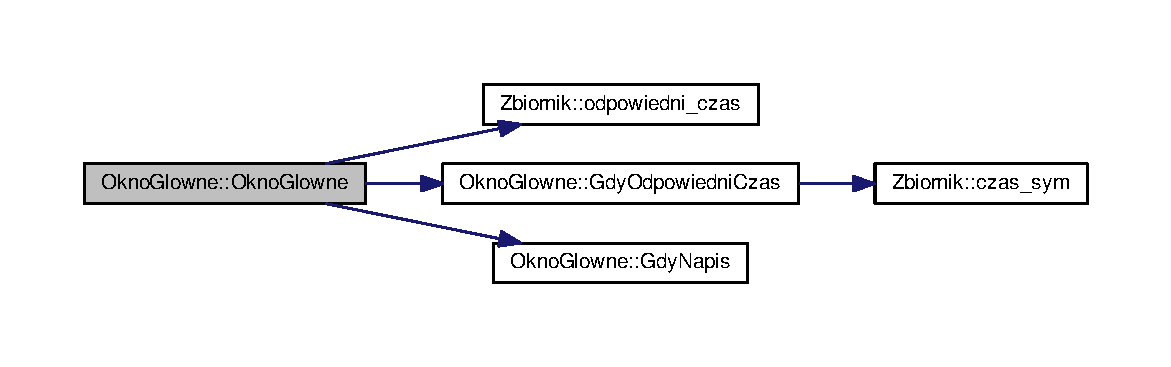
\includegraphics[width=350pt]{class_okno_glowne_a8dcfe4e0f18dfaf0c535c4549991b550_cgraph}
\end{center}
\end{figure}




\subsection{Dokumentacja funkcji składowych}
\hypertarget{class_okno_glowne_a2a59f13292adfead4ac821780220044a}{\index{Okno\-Glowne@{Okno\-Glowne}!Gdy\-Napis@{Gdy\-Napis}}
\index{Gdy\-Napis@{Gdy\-Napis}!OknoGlowne@{Okno\-Glowne}}
\subsubsection[{Gdy\-Napis}]{\setlength{\rightskip}{0pt plus 5cm}void Okno\-Glowne\-::\-Gdy\-Napis (
\begin{DoxyParamCaption}
\item[{const Q\-String \&}]{Napis}
\end{DoxyParamCaption}
)\hspace{0.3cm}{\ttfamily [slot]}}}\label{class_okno_glowne_a2a59f13292adfead4ac821780220044a}
Odpowiada za wyswietlenie napisu na belce statusowej. 
\begin{DoxyParams}[1]{Parametry}
\mbox{\tt in}  & {\em Napis} & -\/ napis do wyswietlenia \\
\hline
\end{DoxyParams}


Definicja w linii 223 pliku okno\-\_\-glowne.\-cpp.



Oto graf wywoływań tej funkcji\-:\nopagebreak
\begin{figure}[H]
\begin{center}
\leavevmode
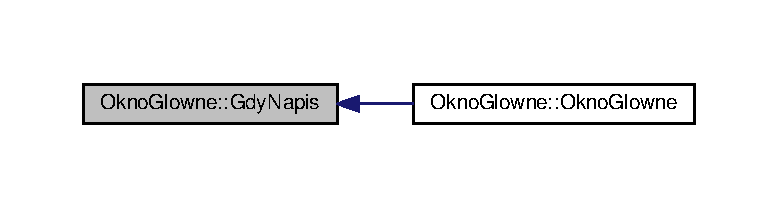
\includegraphics[width=350pt]{class_okno_glowne_a2a59f13292adfead4ac821780220044a_icgraph}
\end{center}
\end{figure}


\hypertarget{class_okno_glowne_a2a49d3696ef8a42325313842768f2c92}{\index{Okno\-Glowne@{Okno\-Glowne}!Gdy\-Odpowiedni\-Czas@{Gdy\-Odpowiedni\-Czas}}
\index{Gdy\-Odpowiedni\-Czas@{Gdy\-Odpowiedni\-Czas}!OknoGlowne@{Okno\-Glowne}}
\subsubsection[{Gdy\-Odpowiedni\-Czas}]{\setlength{\rightskip}{0pt plus 5cm}void Okno\-Glowne\-::\-Gdy\-Odpowiedni\-Czas (
\begin{DoxyParamCaption}
{}
\end{DoxyParamCaption}
)\hspace{0.3cm}{\ttfamily [slot]}}}\label{class_okno_glowne_a2a49d3696ef8a42325313842768f2c92}
Odpowiada za uaktualnienie okienka w odpowiednich momentach. 

Definicja w linii 215 pliku okno\-\_\-glowne.\-cpp.



Oto graf wywoływań tej funkcji\-:\nopagebreak
\begin{figure}[H]
\begin{center}
\leavevmode
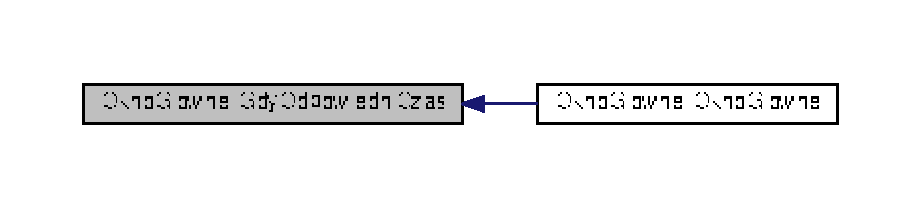
\includegraphics[width=350pt]{class_okno_glowne_a2a49d3696ef8a42325313842768f2c92_icgraph}
\end{center}
\end{figure}


\hypertarget{class_okno_glowne_a8ed8fc49c9c3d3e187639880ce286c88}{\index{Okno\-Glowne@{Okno\-Glowne}!on\-\_\-action\-\_\-\-Save\-\_\-triggered@{on\-\_\-action\-\_\-\-Save\-\_\-triggered}}
\index{on\-\_\-action\-\_\-\-Save\-\_\-triggered@{on\-\_\-action\-\_\-\-Save\-\_\-triggered}!OknoGlowne@{Okno\-Glowne}}
\subsubsection[{on\-\_\-action\-\_\-\-Save\-\_\-triggered}]{\setlength{\rightskip}{0pt plus 5cm}void Okno\-Glowne\-::on\-\_\-action\-\_\-\-Save\-\_\-triggered (
\begin{DoxyParamCaption}
{}
\end{DoxyParamCaption}
)\hspace{0.3cm}{\ttfamily [slot]}}}\label{class_okno_glowne_a8ed8fc49c9c3d3e187639880ce286c88}
Odpowiada za wykonanie odpowiednich czynnosci po przycisnieciu Save. 

Definicja w linii 204 pliku okno\-\_\-glowne.\-cpp.



Oto graf wywołań dla tej funkcji\-:\nopagebreak
\begin{figure}[H]
\begin{center}
\leavevmode
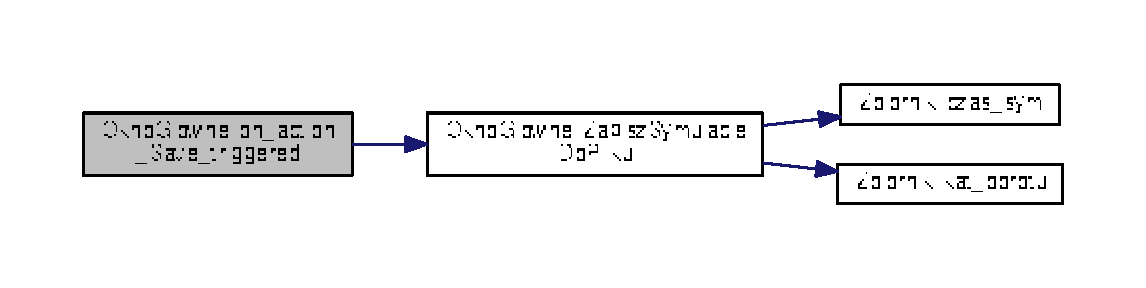
\includegraphics[width=350pt]{class_okno_glowne_a8ed8fc49c9c3d3e187639880ce286c88_cgraph}
\end{center}
\end{figure}


\hypertarget{class_okno_glowne_a0c744f19fcf0e4bcd04a49502864e020}{\index{Okno\-Glowne@{Okno\-Glowne}!on\-\_\-line\-Edit\-\_\-return\-Pressed@{on\-\_\-line\-Edit\-\_\-return\-Pressed}}
\index{on\-\_\-line\-Edit\-\_\-return\-Pressed@{on\-\_\-line\-Edit\-\_\-return\-Pressed}!OknoGlowne@{Okno\-Glowne}}
\subsubsection[{on\-\_\-line\-Edit\-\_\-return\-Pressed}]{\setlength{\rightskip}{0pt plus 5cm}void Okno\-Glowne\-::on\-\_\-line\-Edit\-\_\-return\-Pressed (
\begin{DoxyParamCaption}
{}
\end{DoxyParamCaption}
)\hspace{0.3cm}{\ttfamily [slot]}}}\label{class_okno_glowne_a0c744f19fcf0e4bcd04a49502864e020}
Odpowiada za wczytanie danych z pliku. 

Definicja w linii 191 pliku okno\-\_\-glowne.\-cpp.



Oto graf wywołań dla tej funkcji\-:
\nopagebreak
\begin{figure}[H]
\begin{center}
\leavevmode
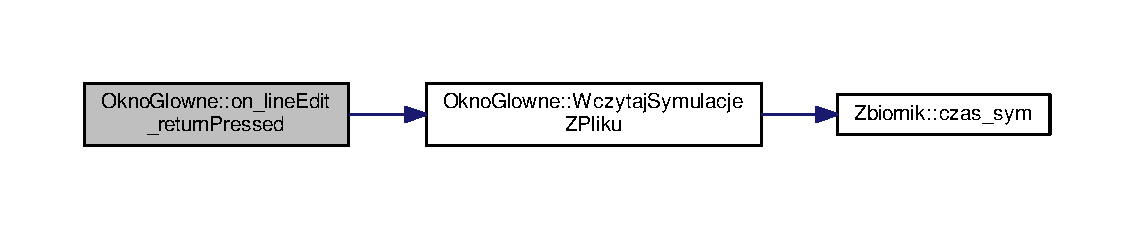
\includegraphics[width=350pt]{class_okno_glowne_a0c744f19fcf0e4bcd04a49502864e020_cgraph}
\end{center}
\end{figure}


\hypertarget{class_okno_glowne_aba5accbf5e231ba194ee0e966b8d7b15}{\index{Okno\-Glowne@{Okno\-Glowne}!on\-\_\-load\-Button\-\_\-clicked@{on\-\_\-load\-Button\-\_\-clicked}}
\index{on\-\_\-load\-Button\-\_\-clicked@{on\-\_\-load\-Button\-\_\-clicked}!OknoGlowne@{Okno\-Glowne}}
\subsubsection[{on\-\_\-load\-Button\-\_\-clicked}]{\setlength{\rightskip}{0pt plus 5cm}void Okno\-Glowne\-::on\-\_\-load\-Button\-\_\-clicked (
\begin{DoxyParamCaption}
{}
\end{DoxyParamCaption}
)\hspace{0.3cm}{\ttfamily [slot]}}}\label{class_okno_glowne_aba5accbf5e231ba194ee0e966b8d7b15}
Odpowiada za wczytanie danych z pliku. 

Definicja w linii 185 pliku okno\-\_\-glowne.\-cpp.



Oto graf wywołań dla tej funkcji\-:\nopagebreak
\begin{figure}[H]
\begin{center}
\leavevmode
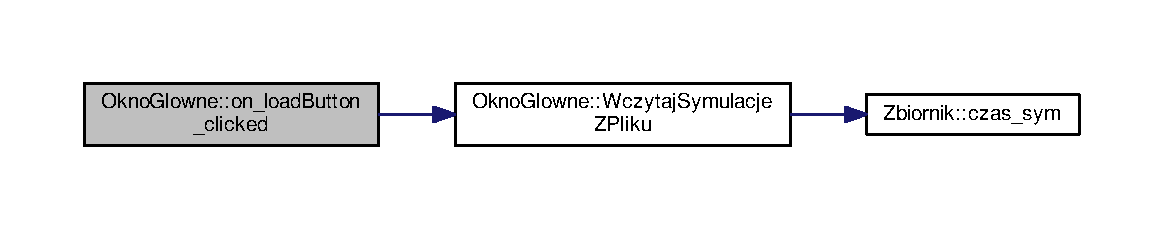
\includegraphics[width=350pt]{class_okno_glowne_aba5accbf5e231ba194ee0e966b8d7b15_cgraph}
\end{center}
\end{figure}


\hypertarget{class_okno_glowne_ae8bd560de9aa835ba8b194b8f7da094c}{\index{Okno\-Glowne@{Okno\-Glowne}!on\-\_\-pause\-Button\-\_\-clicked@{on\-\_\-pause\-Button\-\_\-clicked}}
\index{on\-\_\-pause\-Button\-\_\-clicked@{on\-\_\-pause\-Button\-\_\-clicked}!OknoGlowne@{Okno\-Glowne}}
\subsubsection[{on\-\_\-pause\-Button\-\_\-clicked}]{\setlength{\rightskip}{0pt plus 5cm}void Okno\-Glowne\-::on\-\_\-pause\-Button\-\_\-clicked (
\begin{DoxyParamCaption}
{}
\end{DoxyParamCaption}
)\hspace{0.3cm}{\ttfamily [slot]}}}\label{class_okno_glowne_ae8bd560de9aa835ba8b194b8f7da094c}
Odpowiada za wykonanie odpowiednich czynnosci w trakcie stanu pauza. 

Definicja w linii 177 pliku okno\-\_\-glowne.\-cpp.

\hypertarget{class_okno_glowne_ac837b1f8c8b0288d07987e059966431b}{\index{Okno\-Glowne@{Okno\-Glowne}!on\-\_\-play\-Button\-\_\-clicked@{on\-\_\-play\-Button\-\_\-clicked}}
\index{on\-\_\-play\-Button\-\_\-clicked@{on\-\_\-play\-Button\-\_\-clicked}!OknoGlowne@{Okno\-Glowne}}
\subsubsection[{on\-\_\-play\-Button\-\_\-clicked}]{\setlength{\rightskip}{0pt plus 5cm}void Okno\-Glowne\-::on\-\_\-play\-Button\-\_\-clicked (
\begin{DoxyParamCaption}
{}
\end{DoxyParamCaption}
)\hspace{0.3cm}{\ttfamily [slot]}}}\label{class_okno_glowne_ac837b1f8c8b0288d07987e059966431b}
Odpowiada za wykonanie odpowiednich czynnosci w trakcie stanu play. 

Definicja w linii 167 pliku okno\-\_\-glowne.\-cpp.



Oto graf wywołań dla tej funkcji\-:\nopagebreak
\begin{figure}[H]
\begin{center}
\leavevmode
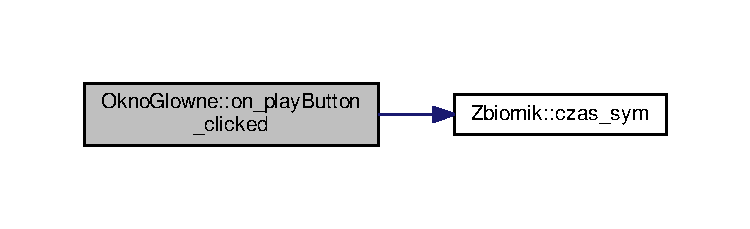
\includegraphics[width=350pt]{class_okno_glowne_ac837b1f8c8b0288d07987e059966431b_cgraph}
\end{center}
\end{figure}


\hypertarget{class_okno_glowne_a726ce3fbe89c3fb7364c39e99c0ad658}{\index{Okno\-Glowne@{Okno\-Glowne}!on\-\_\-slider\-Szybkosc\-Sym\-\_\-value\-Changed@{on\-\_\-slider\-Szybkosc\-Sym\-\_\-value\-Changed}}
\index{on\-\_\-slider\-Szybkosc\-Sym\-\_\-value\-Changed@{on\-\_\-slider\-Szybkosc\-Sym\-\_\-value\-Changed}!OknoGlowne@{Okno\-Glowne}}
\subsubsection[{on\-\_\-slider\-Szybkosc\-Sym\-\_\-value\-Changed}]{\setlength{\rightskip}{0pt plus 5cm}void Okno\-Glowne\-::on\-\_\-slider\-Szybkosc\-Sym\-\_\-value\-Changed (
\begin{DoxyParamCaption}
\item[{int}]{a}
\end{DoxyParamCaption}
)\hspace{0.3cm}{\ttfamily [slot]}}}\label{class_okno_glowne_a726ce3fbe89c3fb7364c39e99c0ad658}
Odpowiada za wykonanie odpowiednich czynnosci po zmianie wartosci slidera. 

Definicja w linii 197 pliku okno\-\_\-glowne.\-cpp.



Oto graf wywołań dla tej funkcji\-:\nopagebreak
\begin{figure}[H]
\begin{center}
\leavevmode
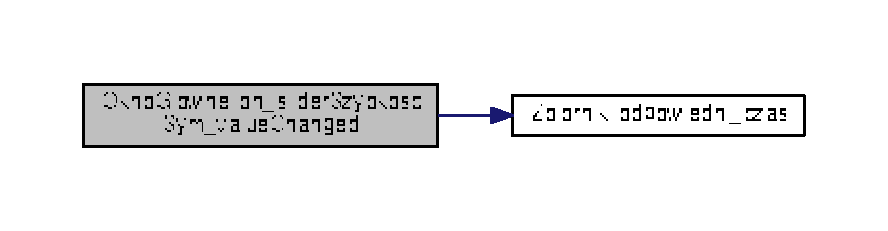
\includegraphics[width=350pt]{class_okno_glowne_a726ce3fbe89c3fb7364c39e99c0ad658_cgraph}
\end{center}
\end{figure}


\hypertarget{class_okno_glowne_a63255adc6263a1ee6f67c96b91446b73}{\index{Okno\-Glowne@{Okno\-Glowne}!on\-\_\-stop\-Button\-\_\-clicked@{on\-\_\-stop\-Button\-\_\-clicked}}
\index{on\-\_\-stop\-Button\-\_\-clicked@{on\-\_\-stop\-Button\-\_\-clicked}!OknoGlowne@{Okno\-Glowne}}
\subsubsection[{on\-\_\-stop\-Button\-\_\-clicked}]{\setlength{\rightskip}{0pt plus 5cm}void Okno\-Glowne\-::on\-\_\-stop\-Button\-\_\-clicked (
\begin{DoxyParamCaption}
{}
\end{DoxyParamCaption}
)\hspace{0.3cm}{\ttfamily [slot]}}}\label{class_okno_glowne_a63255adc6263a1ee6f67c96b91446b73}
Odpowiada za wykonanie odpowiednich czynnosci w trakcie stanu stop. 

Definicja w linii 181 pliku okno\-\_\-glowne.\-cpp.

\hypertarget{class_okno_glowne_a570c795e3829c3bd7896551c0624abe2}{\index{Okno\-Glowne@{Okno\-Glowne}!paint\-Event@{paint\-Event}}
\index{paint\-Event@{paint\-Event}!OknoGlowne@{Okno\-Glowne}}
\subsubsection[{paint\-Event}]{\setlength{\rightskip}{0pt plus 5cm}void Okno\-Glowne\-::paint\-Event (
\begin{DoxyParamCaption}
\item[{Q\-Paint\-Event $\ast$}]{event}
\end{DoxyParamCaption}
)\hspace{0.3cm}{\ttfamily [virtual]}}}\label{class_okno_glowne_a570c795e3829c3bd7896551c0624abe2}
Odziedziczona wirtualna metoda paint\-Event. Rysuje zbiornik i przyciski w nowym miejscu. 
\begin{DoxyParams}[1]{Parametry}
\mbox{\tt in,out}  & {\em event} & -\/ wskaznik obiekt klasy Q\-Paint\-Event \\
\hline
\end{DoxyParams}


Definicja w linii 227 pliku okno\-\_\-glowne.\-cpp.



Oto graf wywołań dla tej funkcji\-:\nopagebreak
\begin{figure}[H]
\begin{center}
\leavevmode
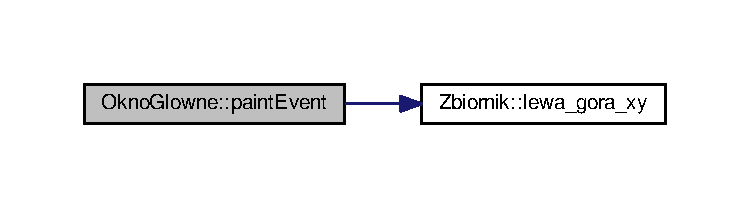
\includegraphics[width=350pt]{class_okno_glowne_a570c795e3829c3bd7896551c0624abe2_cgraph}
\end{center}
\end{figure}


\hypertarget{class_okno_glowne_a1b8098c27e9656235bb056aeb79a8ece}{\index{Okno\-Glowne@{Okno\-Glowne}!Wczytaj\-Symulacje\-Z\-Pliku@{Wczytaj\-Symulacje\-Z\-Pliku}}
\index{Wczytaj\-Symulacje\-Z\-Pliku@{Wczytaj\-Symulacje\-Z\-Pliku}!OknoGlowne@{Okno\-Glowne}}
\subsubsection[{Wczytaj\-Symulacje\-Z\-Pliku}]{\setlength{\rightskip}{0pt plus 5cm}void Okno\-Glowne\-::\-Wczytaj\-Symulacje\-Z\-Pliku (
\begin{DoxyParamCaption}
\item[{const std\-::string}]{nazwa\-\_\-pliku}
\end{DoxyParamCaption}
)}}\label{class_okno_glowne_a1b8098c27e9656235bb056aeb79a8ece}
Wczytuje stan symulacji (czas, liczba czasteczek, dane czasteczek). 

Definicja w linii 266 pliku okno\-\_\-glowne.\-cpp.



Oto graf wywołań dla tej funkcji\-:\nopagebreak
\begin{figure}[H]
\begin{center}
\leavevmode
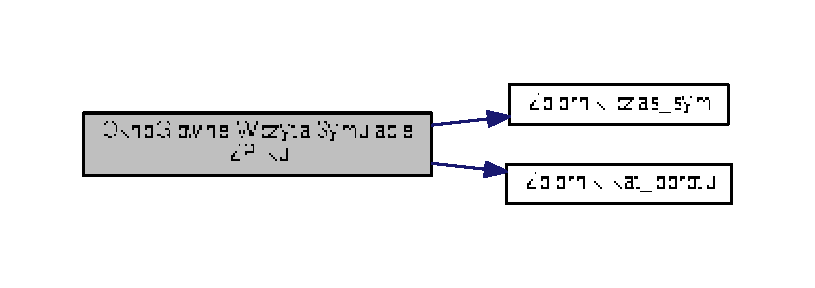
\includegraphics[width=350pt]{class_okno_glowne_a1b8098c27e9656235bb056aeb79a8ece_cgraph}
\end{center}
\end{figure}




Oto graf wywoływań tej funkcji\-:
\nopagebreak
\begin{figure}[H]
\begin{center}
\leavevmode
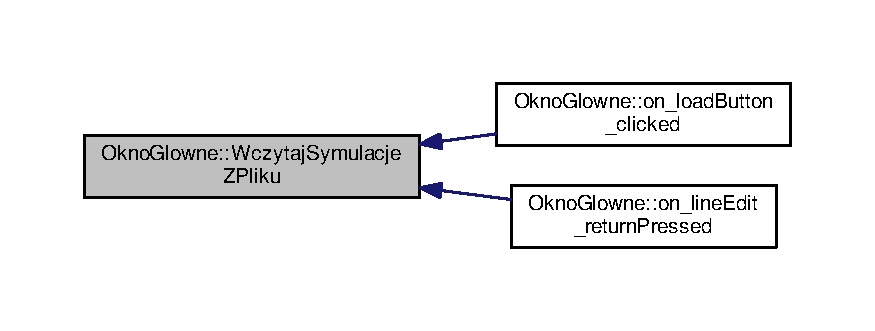
\includegraphics[width=350pt]{class_okno_glowne_a1b8098c27e9656235bb056aeb79a8ece_icgraph}
\end{center}
\end{figure}


\hypertarget{class_okno_glowne_a6062f76fdf15ad8bc0543cfd2a2fe150}{\index{Okno\-Glowne@{Okno\-Glowne}!Zapisz\-Symulacje\-Do\-Pliku@{Zapisz\-Symulacje\-Do\-Pliku}}
\index{Zapisz\-Symulacje\-Do\-Pliku@{Zapisz\-Symulacje\-Do\-Pliku}!OknoGlowne@{Okno\-Glowne}}
\subsubsection[{Zapisz\-Symulacje\-Do\-Pliku}]{\setlength{\rightskip}{0pt plus 5cm}void Okno\-Glowne\-::\-Zapisz\-Symulacje\-Do\-Pliku (
\begin{DoxyParamCaption}
{}
\end{DoxyParamCaption}
)}}\label{class_okno_glowne_a6062f76fdf15ad8bc0543cfd2a2fe150}
Zapisuje aktualny stan symulacji (czas, liczba czasteczek, dane czasteczek) do pliku. 

Definicja w linii 243 pliku okno\-\_\-glowne.\-cpp.



Oto graf wywołań dla tej funkcji\-:\nopagebreak
\begin{figure}[H]
\begin{center}
\leavevmode
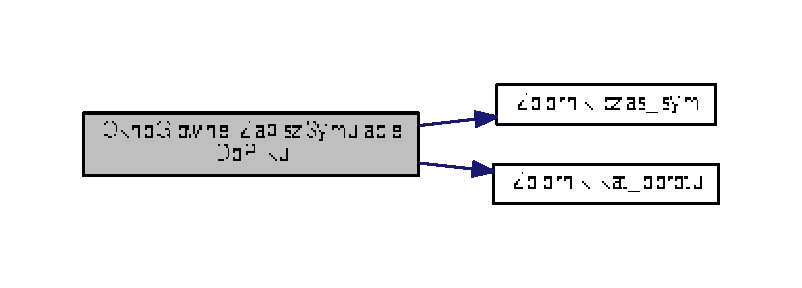
\includegraphics[width=350pt]{class_okno_glowne_a6062f76fdf15ad8bc0543cfd2a2fe150_cgraph}
\end{center}
\end{figure}




Oto graf wywoływań tej funkcji\-:\nopagebreak
\begin{figure}[H]
\begin{center}
\leavevmode
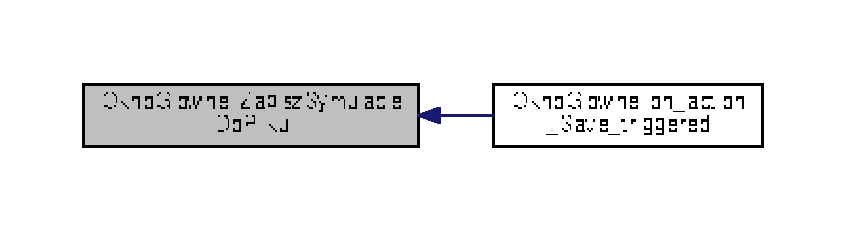
\includegraphics[width=350pt]{class_okno_glowne_a6062f76fdf15ad8bc0543cfd2a2fe150_icgraph}
\end{center}
\end{figure}


\hypertarget{class_okno_glowne_aa602a0c5a940f0af4ab7390bfc1a4b9d}{\index{Okno\-Glowne@{Okno\-Glowne}!Zglos\-Napis@{Zglos\-Napis}}
\index{Zglos\-Napis@{Zglos\-Napis}!OknoGlowne@{Okno\-Glowne}}
\subsubsection[{Zglos\-Napis}]{\setlength{\rightskip}{0pt plus 5cm}void Okno\-Glowne\-::\-Zglos\-Napis (
\begin{DoxyParamCaption}
\item[{const Q\-String \&}]{\-\_\-t1}
\end{DoxyParamCaption}
)\hspace{0.3cm}{\ttfamily [signal]}}}\label{class_okno_glowne_aa602a0c5a940f0af4ab7390bfc1a4b9d}
Sygnal zglaszajacy napis do odpowiedniego slotu. 
\begin{DoxyParams}[1]{Parametry}
\mbox{\tt in}  & {\em \-\_\-t1} & -\/ napis do zgloszenia \\
\hline
\end{DoxyParams}


Definicja w linii 121 pliku moc\-\_\-okno\-\_\-glowne.\-cpp.



Oto graf wywoływań tej funkcji\-:\nopagebreak
\begin{figure}[H]
\begin{center}
\leavevmode
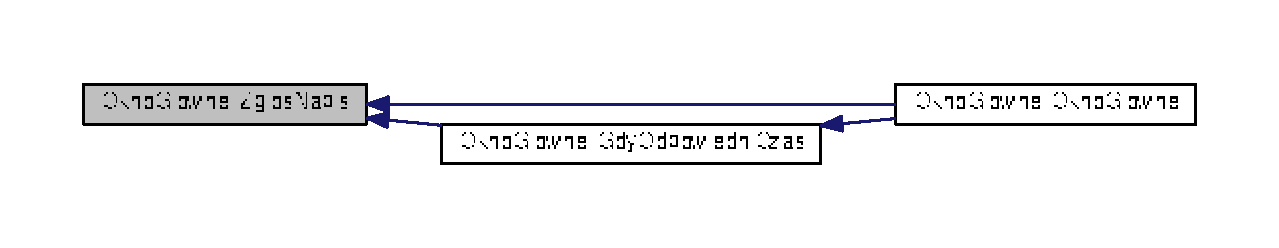
\includegraphics[width=350pt]{class_okno_glowne_aa602a0c5a940f0af4ab7390bfc1a4b9d_icgraph}
\end{center}
\end{figure}




\subsection{Dokumentacja atrybutów składowych}
\hypertarget{class_okno_glowne_a7dae1b25dbade179eb6dfc30ffeab14b}{\index{Okno\-Glowne@{Okno\-Glowne}!\-\_\-old\-\_\-height@{\-\_\-old\-\_\-height}}
\index{\-\_\-old\-\_\-height@{\-\_\-old\-\_\-height}!OknoGlowne@{Okno\-Glowne}}
\subsubsection[{\-\_\-old\-\_\-height}]{\setlength{\rightskip}{0pt plus 5cm}double Okno\-Glowne\-::\-\_\-old\-\_\-height\hspace{0.3cm}{\ttfamily [private]}}}\label{class_okno_glowne_a7dae1b25dbade179eb6dfc30ffeab14b}
Stara wysokosc okienka. 

Definicja w linii 367 pliku okno\-\_\-glowne.\-hh.

\hypertarget{class_okno_glowne_a6a0922607c0970ecdfe8adec7a773c7f}{\index{Okno\-Glowne@{Okno\-Glowne}!\-\_\-old\-\_\-width@{\-\_\-old\-\_\-width}}
\index{\-\_\-old\-\_\-width@{\-\_\-old\-\_\-width}!OknoGlowne@{Okno\-Glowne}}
\subsubsection[{\-\_\-old\-\_\-width}]{\setlength{\rightskip}{0pt plus 5cm}double Okno\-Glowne\-::\-\_\-old\-\_\-width\hspace{0.3cm}{\ttfamily [private]}}}\label{class_okno_glowne_a6a0922607c0970ecdfe8adec7a773c7f}
Stara szerokosc okienka. 

Definicja w linii 361 pliku okno\-\_\-glowne.\-hh.

\hypertarget{class_okno_glowne_a5d047f90666212f58e69d11af3285d9b}{\index{Okno\-Glowne@{Okno\-Glowne}!\-\_\-\-Stoper@{\-\_\-\-Stoper}}
\index{\-\_\-\-Stoper@{\-\_\-\-Stoper}!OknoGlowne@{Okno\-Glowne}}
\subsubsection[{\-\_\-\-Stoper}]{\setlength{\rightskip}{0pt plus 5cm}Q\-Timer Okno\-Glowne\-::\-\_\-\-Stoper}}\label{class_okno_glowne_a5d047f90666212f58e69d11af3285d9b}
Miernik czasu. 

Definicja w linii 353 pliku okno\-\_\-glowne.\-hh.

\hypertarget{class_okno_glowne_a579ef9901f57057368cb522ea5a9a5c3}{\index{Okno\-Glowne@{Okno\-Glowne}!action\-\_\-\-Exit@{action\-\_\-\-Exit}}
\index{action\-\_\-\-Exit@{action\-\_\-\-Exit}!OknoGlowne@{Okno\-Glowne}}
\subsubsection[{action\-\_\-\-Exit}]{\setlength{\rightskip}{0pt plus 5cm}Q\-Action$\ast$ Okno\-Glowne\-::action\-\_\-\-Exit\hspace{0.3cm}{\ttfamily [private]}}}\label{class_okno_glowne_a579ef9901f57057368cb522ea5a9a5c3}
Wskaznik na akcje przycisku menu Exit. 

Definicja w linii 212 pliku okno\-\_\-glowne.\-hh.

\hypertarget{class_okno_glowne_a2c2d825b6e5e0faa5eb368be4fc73b78}{\index{Okno\-Glowne@{Okno\-Glowne}!action\-\_\-\-Save@{action\-\_\-\-Save}}
\index{action\-\_\-\-Save@{action\-\_\-\-Save}!OknoGlowne@{Okno\-Glowne}}
\subsubsection[{action\-\_\-\-Save}]{\setlength{\rightskip}{0pt plus 5cm}Q\-Action$\ast$ Okno\-Glowne\-::action\-\_\-\-Save\hspace{0.3cm}{\ttfamily [private]}}}\label{class_okno_glowne_a2c2d825b6e5e0faa5eb368be4fc73b78}
Wskaznik na akcje przycisku menu Save. 

Definicja w linii 205 pliku okno\-\_\-glowne.\-hh.

\hypertarget{class_okno_glowne_aacb5ddb6d0eb560a47917cc1b457239a}{\index{Okno\-Glowne@{Okno\-Glowne}!horizontal\-Layout@{horizontal\-Layout}}
\index{horizontal\-Layout@{horizontal\-Layout}!OknoGlowne@{Okno\-Glowne}}
\subsubsection[{horizontal\-Layout}]{\setlength{\rightskip}{0pt plus 5cm}Q\-H\-Box\-Layout$\ast$ Okno\-Glowne\-::horizontal\-Layout\hspace{0.3cm}{\ttfamily [private]}}}\label{class_okno_glowne_aacb5ddb6d0eb560a47917cc1b457239a}
Wskaznik na obszar do horyzontalnego rozmieszczenia przyciskow. 

Definicja w linii 254 pliku okno\-\_\-glowne.\-hh.

\hypertarget{class_okno_glowne_a12ac2d00b9ca186176ccc710a928a723}{\index{Okno\-Glowne@{Okno\-Glowne}!horizontal\-Layout\-Widget@{horizontal\-Layout\-Widget}}
\index{horizontal\-Layout\-Widget@{horizontal\-Layout\-Widget}!OknoGlowne@{Okno\-Glowne}}
\subsubsection[{horizontal\-Layout\-Widget}]{\setlength{\rightskip}{0pt plus 5cm}Q\-Widget$\ast$ Okno\-Glowne\-::horizontal\-Layout\-Widget\hspace{0.3cm}{\ttfamily [private]}}}\label{class_okno_glowne_a12ac2d00b9ca186176ccc710a928a723}
Wskaznik na widget odpowiedzialny za horyzontalne wyswietlenie przyciskow. 

Definicja w linii 261 pliku okno\-\_\-glowne.\-hh.

\hypertarget{class_okno_glowne_aca07e1dc5cbe30d6952f9b952073bb79}{\index{Okno\-Glowne@{Okno\-Glowne}!label\-Czas\-Sym@{label\-Czas\-Sym}}
\index{label\-Czas\-Sym@{label\-Czas\-Sym}!OknoGlowne@{Okno\-Glowne}}
\subsubsection[{label\-Czas\-Sym}]{\setlength{\rightskip}{0pt plus 5cm}Q\-Label$\ast$ Okno\-Glowne\-::label\-Czas\-Sym\hspace{0.3cm}{\ttfamily [private]}}}\label{class_okno_glowne_aca07e1dc5cbe30d6952f9b952073bb79}
Etykieta dla czasu symulacji. 

Definicja w linii 317 pliku okno\-\_\-glowne.\-hh.

\hypertarget{class_okno_glowne_ab01460f1222d0ec2892abf21efb23078}{\index{Okno\-Glowne@{Okno\-Glowne}!label\-Liczba\-Czasteczek@{label\-Liczba\-Czasteczek}}
\index{label\-Liczba\-Czasteczek@{label\-Liczba\-Czasteczek}!OknoGlowne@{Okno\-Glowne}}
\subsubsection[{label\-Liczba\-Czasteczek}]{\setlength{\rightskip}{0pt plus 5cm}Q\-Label$\ast$ Okno\-Glowne\-::label\-Liczba\-Czasteczek\hspace{0.3cm}{\ttfamily [private]}}}\label{class_okno_glowne_ab01460f1222d0ec2892abf21efb23078}
Etykieta dla liczby symulowanych czasteczek. 

Definicja w linii 331 pliku okno\-\_\-glowne.\-hh.

\hypertarget{class_okno_glowne_ad7b0708ffdf61f3bef1349cc353a6c4e}{\index{Okno\-Glowne@{Okno\-Glowne}!label\-Szybkosc\-Sym@{label\-Szybkosc\-Sym}}
\index{label\-Szybkosc\-Sym@{label\-Szybkosc\-Sym}!OknoGlowne@{Okno\-Glowne}}
\subsubsection[{label\-Szybkosc\-Sym}]{\setlength{\rightskip}{0pt plus 5cm}Q\-Label$\ast$ Okno\-Glowne\-::label\-Szybkosc\-Sym\hspace{0.3cm}{\ttfamily [private]}}}\label{class_okno_glowne_ad7b0708ffdf61f3bef1349cc353a6c4e}
Etykieta dla szybkosci symulacji. 

Definicja w linii 310 pliku okno\-\_\-glowne.\-hh.

\hypertarget{class_okno_glowne_ab34fefe738e38b1b0d4ce764481cc0c6}{\index{Okno\-Glowne@{Okno\-Glowne}!lcd\-Czas\-Sym@{lcd\-Czas\-Sym}}
\index{lcd\-Czas\-Sym@{lcd\-Czas\-Sym}!OknoGlowne@{Okno\-Glowne}}
\subsubsection[{lcd\-Czas\-Sym}]{\setlength{\rightskip}{0pt plus 5cm}Q\-L\-C\-D\-Number$\ast$ Okno\-Glowne\-::lcd\-Czas\-Sym\hspace{0.3cm}{\ttfamily [private]}}}\label{class_okno_glowne_ab34fefe738e38b1b0d4ce764481cc0c6}
Wskaznik na L\-C\-D z szybkoscia symulacji. Wyswietla jej czas trwania. 

Definicja w linii 324 pliku okno\-\_\-glowne.\-hh.

\hypertarget{class_okno_glowne_adbdd9fc009725804e015d267dc8375dc}{\index{Okno\-Glowne@{Okno\-Glowne}!lcd\-Liczba\-Czasteczek@{lcd\-Liczba\-Czasteczek}}
\index{lcd\-Liczba\-Czasteczek@{lcd\-Liczba\-Czasteczek}!OknoGlowne@{Okno\-Glowne}}
\subsubsection[{lcd\-Liczba\-Czasteczek}]{\setlength{\rightskip}{0pt plus 5cm}Q\-L\-C\-D\-Number$\ast$ Okno\-Glowne\-::lcd\-Liczba\-Czasteczek\hspace{0.3cm}{\ttfamily [private]}}}\label{class_okno_glowne_adbdd9fc009725804e015d267dc8375dc}
Wyswietla liczbe symulowanych czasteczek. 

Definicja w linii 338 pliku okno\-\_\-glowne.\-hh.

\hypertarget{class_okno_glowne_ab100c00d4ba33d896fd0985ac366296a}{\index{Okno\-Glowne@{Okno\-Glowne}!lcd\-Szybkosc\-Sym@{lcd\-Szybkosc\-Sym}}
\index{lcd\-Szybkosc\-Sym@{lcd\-Szybkosc\-Sym}!OknoGlowne@{Okno\-Glowne}}
\subsubsection[{lcd\-Szybkosc\-Sym}]{\setlength{\rightskip}{0pt plus 5cm}Q\-L\-C\-D\-Number$\ast$ Okno\-Glowne\-::lcd\-Szybkosc\-Sym\hspace{0.3cm}{\ttfamily [private]}}}\label{class_okno_glowne_ab100c00d4ba33d896fd0985ac366296a}
Wskaznik na L\-C\-D z szybkoscia symulacji. Wyswietla jej szybkosc. 

Definicja w linii 303 pliku okno\-\_\-glowne.\-hh.

\hypertarget{class_okno_glowne_ae615cbd9c9f9ab06b365c4692ff68729}{\index{Okno\-Glowne@{Okno\-Glowne}!licznik\-\_\-plikow@{licznik\-\_\-plikow}}
\index{licznik\-\_\-plikow@{licznik\-\_\-plikow}!OknoGlowne@{Okno\-Glowne}}
\subsubsection[{licznik\-\_\-plikow}]{\setlength{\rightskip}{0pt plus 5cm}int Okno\-Glowne\-::licznik\-\_\-plikow\hspace{0.3cm}{\ttfamily [static]}, {\ttfamily [private]}}}\label{class_okno_glowne_ae615cbd9c9f9ab06b365c4692ff68729}
Sluzy do generowania unikatowych nazw plikow wyjsciowych. 

Definicja w linii 184 pliku okno\-\_\-glowne.\-hh.

\hypertarget{class_okno_glowne_a0112b8be70a26552b03f38fab43a3301}{\index{Okno\-Glowne@{Okno\-Glowne}!line\-Edit@{line\-Edit}}
\index{line\-Edit@{line\-Edit}!OknoGlowne@{Okno\-Glowne}}
\subsubsection[{line\-Edit}]{\setlength{\rightskip}{0pt plus 5cm}Q\-Line\-Edit$\ast$ Okno\-Glowne\-::line\-Edit\hspace{0.3cm}{\ttfamily [private]}}}\label{class_okno_glowne_a0112b8be70a26552b03f38fab43a3301}
Wskazuje linijke do wpisywania tekstu. 

Definicja w linii 345 pliku okno\-\_\-glowne.\-hh.

\hypertarget{class_okno_glowne_accbadc3bc4d418cfe1bce2be61881917}{\index{Okno\-Glowne@{Okno\-Glowne}!load\-Button@{load\-Button}}
\index{load\-Button@{load\-Button}!OknoGlowne@{Okno\-Glowne}}
\subsubsection[{load\-Button}]{\setlength{\rightskip}{0pt plus 5cm}Q\-Push\-Button$\ast$ Okno\-Glowne\-::load\-Button\hspace{0.3cm}{\ttfamily [private]}}}\label{class_okno_glowne_accbadc3bc4d418cfe1bce2be61881917}
Wskaznik na przycisk Wczytaj. Wczytuje symulacje. 

Definicja w linii 289 pliku okno\-\_\-glowne.\-hh.

\hypertarget{class_okno_glowne_a93afadd0ec22ce6a7e29acc5dd2423a2}{\index{Okno\-Glowne@{Okno\-Glowne}!menu\-\_\-\-Edit@{menu\-\_\-\-Edit}}
\index{menu\-\_\-\-Edit@{menu\-\_\-\-Edit}!OknoGlowne@{Okno\-Glowne}}
\subsubsection[{menu\-\_\-\-Edit}]{\setlength{\rightskip}{0pt plus 5cm}Q\-Menu$\ast$ Okno\-Glowne\-::menu\-\_\-\-Edit\hspace{0.3cm}{\ttfamily [private]}}}\label{class_okno_glowne_a93afadd0ec22ce6a7e29acc5dd2423a2}
Wskaznik na akcje przycisku menu Edit. 

Definicja w linii 226 pliku okno\-\_\-glowne.\-hh.

\hypertarget{class_okno_glowne_a1ba162db2d0b06b0f8963e61b3806875}{\index{Okno\-Glowne@{Okno\-Glowne}!menu\-\_\-\-File@{menu\-\_\-\-File}}
\index{menu\-\_\-\-File@{menu\-\_\-\-File}!OknoGlowne@{Okno\-Glowne}}
\subsubsection[{menu\-\_\-\-File}]{\setlength{\rightskip}{0pt plus 5cm}Q\-Menu$\ast$ Okno\-Glowne\-::menu\-\_\-\-File\hspace{0.3cm}{\ttfamily [private]}}}\label{class_okno_glowne_a1ba162db2d0b06b0f8963e61b3806875}
Wskaznik na akcje przycisku menu File. 

Definicja w linii 219 pliku okno\-\_\-glowne.\-hh.

\hypertarget{class_okno_glowne_ab17be6714913af0cdf4e7de7cb6210d1}{\index{Okno\-Glowne@{Okno\-Glowne}!menu\-\_\-\-Help@{menu\-\_\-\-Help}}
\index{menu\-\_\-\-Help@{menu\-\_\-\-Help}!OknoGlowne@{Okno\-Glowne}}
\subsubsection[{menu\-\_\-\-Help}]{\setlength{\rightskip}{0pt plus 5cm}Q\-Menu$\ast$ Okno\-Glowne\-::menu\-\_\-\-Help\hspace{0.3cm}{\ttfamily [private]}}}\label{class_okno_glowne_ab17be6714913af0cdf4e7de7cb6210d1}
Wskaznik na akcje przycisku menu Help. 

Definicja w linii 233 pliku okno\-\_\-glowne.\-hh.

\hypertarget{class_okno_glowne_a5a87098d9d4bd868670f5a5e72023a0a}{\index{Okno\-Glowne@{Okno\-Glowne}!menu\-Bar@{menu\-Bar}}
\index{menu\-Bar@{menu\-Bar}!OknoGlowne@{Okno\-Glowne}}
\subsubsection[{menu\-Bar}]{\setlength{\rightskip}{0pt plus 5cm}Q\-Menu\-Bar$\ast$ Okno\-Glowne\-::menu\-Bar\hspace{0.3cm}{\ttfamily [private]}}}\label{class_okno_glowne_a5a87098d9d4bd868670f5a5e72023a0a}
Wskaznik na pasek menu. 

Definicja w linii 198 pliku okno\-\_\-glowne.\-hh.

\hypertarget{class_okno_glowne_a0dde8df8a49b8f47f17f8e748fd15967}{\index{Okno\-Glowne@{Okno\-Glowne}!pause\-Button@{pause\-Button}}
\index{pause\-Button@{pause\-Button}!OknoGlowne@{Okno\-Glowne}}
\subsubsection[{pause\-Button}]{\setlength{\rightskip}{0pt plus 5cm}Q\-Push\-Button$\ast$ Okno\-Glowne\-::pause\-Button\hspace{0.3cm}{\ttfamily [private]}}}\label{class_okno_glowne_a0dde8df8a49b8f47f17f8e748fd15967}
Wskaznik na przycisk pause. Wstrzymuje symulacje. 

Definicja w linii 275 pliku okno\-\_\-glowne.\-hh.

\hypertarget{class_okno_glowne_a50f936486c1bc3b3278823a8eb90841e}{\index{Okno\-Glowne@{Okno\-Glowne}!play\-Button@{play\-Button}}
\index{play\-Button@{play\-Button}!OknoGlowne@{Okno\-Glowne}}
\subsubsection[{play\-Button}]{\setlength{\rightskip}{0pt plus 5cm}Q\-Push\-Button$\ast$ Okno\-Glowne\-::play\-Button\hspace{0.3cm}{\ttfamily [private]}}}\label{class_okno_glowne_a50f936486c1bc3b3278823a8eb90841e}
Wskaznik na przycisk play. Uruchamia symulacje. 

Definicja w linii 268 pliku okno\-\_\-glowne.\-hh.

\hypertarget{class_okno_glowne_a85328893065393400d5a0344004ca78b}{\index{Okno\-Glowne@{Okno\-Glowne}!slider\-Szybkosc\-Sym@{slider\-Szybkosc\-Sym}}
\index{slider\-Szybkosc\-Sym@{slider\-Szybkosc\-Sym}!OknoGlowne@{Okno\-Glowne}}
\subsubsection[{slider\-Szybkosc\-Sym}]{\setlength{\rightskip}{0pt plus 5cm}Q\-Slider$\ast$ Okno\-Glowne\-::slider\-Szybkosc\-Sym\hspace{0.3cm}{\ttfamily [private]}}}\label{class_okno_glowne_a85328893065393400d5a0344004ca78b}
Wskaznik na slider. Steruje szybkoscia symulacji. 

Definicja w linii 296 pliku okno\-\_\-glowne.\-hh.

\hypertarget{class_okno_glowne_a40a10989bc6b318ac24e2457d7adb53b}{\index{Okno\-Glowne@{Okno\-Glowne}!status\-Bar@{status\-Bar}}
\index{status\-Bar@{status\-Bar}!OknoGlowne@{Okno\-Glowne}}
\subsubsection[{status\-Bar}]{\setlength{\rightskip}{0pt plus 5cm}Q\-Status\-Bar$\ast$ Okno\-Glowne\-::status\-Bar\hspace{0.3cm}{\ttfamily [private]}}}\label{class_okno_glowne_a40a10989bc6b318ac24e2457d7adb53b}
Wskaznik na pasek statusowy. 

Definicja w linii 240 pliku okno\-\_\-glowne.\-hh.

\hypertarget{class_okno_glowne_a3051d73dc0e0a27dc30ada43cc6b63c4}{\index{Okno\-Glowne@{Okno\-Glowne}!stop\-Button@{stop\-Button}}
\index{stop\-Button@{stop\-Button}!OknoGlowne@{Okno\-Glowne}}
\subsubsection[{stop\-Button}]{\setlength{\rightskip}{0pt plus 5cm}Q\-Push\-Button$\ast$ Okno\-Glowne\-::stop\-Button\hspace{0.3cm}{\ttfamily [private]}}}\label{class_okno_glowne_a3051d73dc0e0a27dc30ada43cc6b63c4}
Wskaznik na przycisk stop. Zatrzymuje symulacje. 

Definicja w linii 282 pliku okno\-\_\-glowne.\-hh.

\hypertarget{class_okno_glowne_a6a37dd1f32605092fff7feac712bf429}{\index{Okno\-Glowne@{Okno\-Glowne}!tool\-Bar@{tool\-Bar}}
\index{tool\-Bar@{tool\-Bar}!OknoGlowne@{Okno\-Glowne}}
\subsubsection[{tool\-Bar}]{\setlength{\rightskip}{0pt plus 5cm}Q\-Tool\-Bar$\ast$ Okno\-Glowne\-::tool\-Bar\hspace{0.3cm}{\ttfamily [private]}}}\label{class_okno_glowne_a6a37dd1f32605092fff7feac712bf429}
Wskaznik na pasek narzedziowy. 

Definicja w linii 247 pliku okno\-\_\-glowne.\-hh.

\hypertarget{class_okno_glowne_af2d1275209898ebdd5ab9de8ef78dffd}{\index{Okno\-Glowne@{Okno\-Glowne}!w\-Zbiornik@{w\-Zbiornik}}
\index{w\-Zbiornik@{w\-Zbiornik}!OknoGlowne@{Okno\-Glowne}}
\subsubsection[{w\-Zbiornik}]{\setlength{\rightskip}{0pt plus 5cm}{\bf Zbiornik}$\ast$ Okno\-Glowne\-::w\-Zbiornik\hspace{0.3cm}{\ttfamily [private]}}}\label{class_okno_glowne_af2d1275209898ebdd5ab9de8ef78dffd}
Wskaznik na zbiornik. 

Definicja w linii 191 pliku okno\-\_\-glowne.\-hh.



Dokumentacja dla tej klasy została wygenerowana z plików\-:\begin{DoxyCompactItemize}
\item 
\hyperlink{okno__glowne_8hh}{okno\-\_\-glowne.\-hh}\item 
\hyperlink{moc__okno__glowne_8cpp}{moc\-\_\-okno\-\_\-glowne.\-cpp}\item 
\hyperlink{okno__glowne_8cpp}{okno\-\_\-glowne.\-cpp}\end{DoxyCompactItemize}

\hypertarget{structparams__t}{\section{Dokumentacja struktury params\-\_\-t}
\label{structparams__t}\index{params\-\_\-t@{params\-\_\-t}}
}


Parametry symulacji.  




{\ttfamily \#include $<$simulation.\-hh$>$}

\subsection*{Atrybuty publiczne}
\begin{DoxyCompactItemize}
\item 
unsigned \hyperlink{structparams__t_a2cecc28f4ca024657cf567047e2aba59}{nframes}
\begin{DoxyCompactList}\small\item\em Liczba ramek -\/ tylko w trybie standalone. \end{DoxyCompactList}\item 
unsigned \hyperlink{structparams__t_a06a1a567fd5ba13905514227e2bb710a}{npframe}
\begin{DoxyCompactList}\small\item\em Liczba kroków na ramkę \end{DoxyCompactList}\item 
float \hyperlink{structparams__t_a27d76064f2ae0cb93a0956027cfcc19b}{h}
\begin{DoxyCompactList}\small\item\em Rozmiar cząstki. \end{DoxyCompactList}\item 
float \hyperlink{structparams__t_a81fc6596e9b1446442ebf3eef2c3fb01}{dt}
\begin{DoxyCompactList}\small\item\em Najmniejsza różnica czasu. \end{DoxyCompactList}\item 
float \hyperlink{structparams__t_a2eb309edb681d0a998f23fc692a73781}{rho0}
\begin{DoxyCompactList}\small\item\em Gęstość cieczy. \end{DoxyCompactList}\item 
float \hyperlink{structparams__t_a97ee2783cf89cee1151be3250e9054b3}{k}
\begin{DoxyCompactList}\small\item\em Współczynnik K. \end{DoxyCompactList}\item 
float \hyperlink{structparams__t_a971359c29b2f946b477e4a1b3605fa3f}{mu}
\begin{DoxyCompactList}\small\item\em Lepkość \end{DoxyCompactList}\item 
float \hyperlink{structparams__t_a9f3f70c0cdedcb053c9d45c2e41e67b6}{gx}
\begin{DoxyCompactList}\small\item\em Grawitacja w poziomie. \end{DoxyCompactList}\item 
float \hyperlink{structparams__t_a0da484b4cc6a542875aa7b92e200f507}{gy}
\begin{DoxyCompactList}\small\item\em Grawitacja w pionie. \end{DoxyCompactList}\item 
float \hyperlink{structparams__t_afe4a59fe43565a71a0a7a155714e2af1}{mass}
\begin{DoxyCompactList}\small\item\em Masa cząstki. \end{DoxyCompactList}\end{DoxyCompactItemize}


\subsection{Opis szczegółowy}
Struktura przechowuje parametry symulacji 

Definicja w linii 34 pliku simulation.\-hh.



\subsection{Dokumentacja atrybutów składowych}
\hypertarget{structparams__t_a81fc6596e9b1446442ebf3eef2c3fb01}{\index{params\-\_\-t@{params\-\_\-t}!dt@{dt}}
\index{dt@{dt}!params_t@{params\-\_\-t}}
\subsubsection[{dt}]{\setlength{\rightskip}{0pt plus 5cm}float params\-\_\-t\-::dt}}\label{structparams__t_a81fc6596e9b1446442ebf3eef2c3fb01}


Definicja w linii 38 pliku simulation.\-hh.

\hypertarget{structparams__t_a9f3f70c0cdedcb053c9d45c2e41e67b6}{\index{params\-\_\-t@{params\-\_\-t}!gx@{gx}}
\index{gx@{gx}!params_t@{params\-\_\-t}}
\subsubsection[{gx}]{\setlength{\rightskip}{0pt plus 5cm}float params\-\_\-t\-::gx}}\label{structparams__t_a9f3f70c0cdedcb053c9d45c2e41e67b6}


Definicja w linii 42 pliku simulation.\-hh.

\hypertarget{structparams__t_a0da484b4cc6a542875aa7b92e200f507}{\index{params\-\_\-t@{params\-\_\-t}!gy@{gy}}
\index{gy@{gy}!params_t@{params\-\_\-t}}
\subsubsection[{gy}]{\setlength{\rightskip}{0pt plus 5cm}float params\-\_\-t\-::gy}}\label{structparams__t_a0da484b4cc6a542875aa7b92e200f507}


Definicja w linii 43 pliku simulation.\-hh.

\hypertarget{structparams__t_a27d76064f2ae0cb93a0956027cfcc19b}{\index{params\-\_\-t@{params\-\_\-t}!h@{h}}
\index{h@{h}!params_t@{params\-\_\-t}}
\subsubsection[{h}]{\setlength{\rightskip}{0pt plus 5cm}float params\-\_\-t\-::h}}\label{structparams__t_a27d76064f2ae0cb93a0956027cfcc19b}


Definicja w linii 37 pliku simulation.\-hh.

\hypertarget{structparams__t_a97ee2783cf89cee1151be3250e9054b3}{\index{params\-\_\-t@{params\-\_\-t}!k@{k}}
\index{k@{k}!params_t@{params\-\_\-t}}
\subsubsection[{k}]{\setlength{\rightskip}{0pt plus 5cm}float params\-\_\-t\-::k}}\label{structparams__t_a97ee2783cf89cee1151be3250e9054b3}


Definicja w linii 40 pliku simulation.\-hh.

\hypertarget{structparams__t_afe4a59fe43565a71a0a7a155714e2af1}{\index{params\-\_\-t@{params\-\_\-t}!mass@{mass}}
\index{mass@{mass}!params_t@{params\-\_\-t}}
\subsubsection[{mass}]{\setlength{\rightskip}{0pt plus 5cm}float params\-\_\-t\-::mass}}\label{structparams__t_afe4a59fe43565a71a0a7a155714e2af1}


Definicja w linii 44 pliku simulation.\-hh.

\hypertarget{structparams__t_a971359c29b2f946b477e4a1b3605fa3f}{\index{params\-\_\-t@{params\-\_\-t}!mu@{mu}}
\index{mu@{mu}!params_t@{params\-\_\-t}}
\subsubsection[{mu}]{\setlength{\rightskip}{0pt plus 5cm}float params\-\_\-t\-::mu}}\label{structparams__t_a971359c29b2f946b477e4a1b3605fa3f}


Definicja w linii 41 pliku simulation.\-hh.

\hypertarget{structparams__t_a2cecc28f4ca024657cf567047e2aba59}{\index{params\-\_\-t@{params\-\_\-t}!nframes@{nframes}}
\index{nframes@{nframes}!params_t@{params\-\_\-t}}
\subsubsection[{nframes}]{\setlength{\rightskip}{0pt plus 5cm}unsigned params\-\_\-t\-::nframes}}\label{structparams__t_a2cecc28f4ca024657cf567047e2aba59}


Definicja w linii 35 pliku simulation.\-hh.

\hypertarget{structparams__t_a06a1a567fd5ba13905514227e2bb710a}{\index{params\-\_\-t@{params\-\_\-t}!npframe@{npframe}}
\index{npframe@{npframe}!params_t@{params\-\_\-t}}
\subsubsection[{npframe}]{\setlength{\rightskip}{0pt plus 5cm}unsigned params\-\_\-t\-::npframe}}\label{structparams__t_a06a1a567fd5ba13905514227e2bb710a}


Definicja w linii 36 pliku simulation.\-hh.

\hypertarget{structparams__t_a2eb309edb681d0a998f23fc692a73781}{\index{params\-\_\-t@{params\-\_\-t}!rho0@{rho0}}
\index{rho0@{rho0}!params_t@{params\-\_\-t}}
\subsubsection[{rho0}]{\setlength{\rightskip}{0pt plus 5cm}float params\-\_\-t\-::rho0}}\label{structparams__t_a2eb309edb681d0a998f23fc692a73781}


Definicja w linii 39 pliku simulation.\-hh.



Dokumentacja dla tej struktury została wygenerowana z pliku\-:\begin{DoxyCompactItemize}
\item 
\hyperlink{simulation_8hh}{simulation.\-hh}\end{DoxyCompactItemize}

\hypertarget{classsimulation}{\section{Dokumentacja klasy simulation}
\label{classsimulation}\index{simulation@{simulation}}
}


backend symulacji  




{\ttfamily \#include $<$simulation.\-hh$>$}



Diagram współpracy dla simulation\-:\nopagebreak
\begin{figure}[H]
\begin{center}
\leavevmode
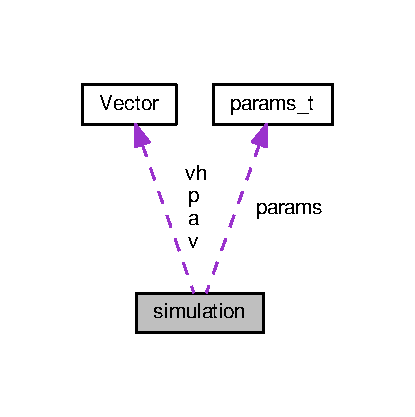
\includegraphics[width=199pt]{classsimulation__coll__graph}
\end{center}
\end{figure}
\subsection*{Metody publiczne}
\begin{DoxyCompactItemize}
\item 
\hyperlink{classsimulation_a30fdcc611ae9a656a3aebb8445e4607d}{simulation} (const unsigned \&\-\_\-n, \hyperlink{structparams__t}{params\-\_\-t} $\ast$\-\_\-param)
\begin{DoxyCompactList}\small\item\em konstruktor klasy \end{DoxyCompactList}\item 
void \hyperlink{classsimulation_a7679fcd9a25d6cb5597338d054a30684}{compute\-Density} (\hyperlink{structparams__t}{params\-\_\-t} $\ast$\-\_\-p)
\begin{DoxyCompactList}\small\item\em wylicza przybliżenia gęstości \end{DoxyCompactList}\item 
void \hyperlink{classsimulation_a16b945b81e27680a709fffd8663bf856}{compute\-Accel} (\hyperlink{structparams__t}{params\-\_\-t} $\ast$\hyperlink{classsimulation_a861b82cc3c0e7e58abfba464a133dae3}{params})
\begin{DoxyCompactList}\small\item\em wylicza przyspieszenia cząstek \end{DoxyCompactList}\item 
void \hyperlink{classsimulation_a353d4dd3a66197360e882bc29a6fef0b}{damp\-Reflect} (float \-\_\-barrier, unsigned i, float \&(Vector\-::$\ast$getter)())
\begin{DoxyCompactList}\small\item\em odbija cząstkę od powierzchni \end{DoxyCompactList}\item 
void \hyperlink{classsimulation_a9cb3fe3f985ceb039736a666923a20b5}{reflect\-Particles} ()
\begin{DoxyCompactList}\small\item\em szuka kolizji cząstek ze ścianami naczynia \end{DoxyCompactList}\item 
void \hyperlink{classsimulation_a300e67649652f2ae9337af3d5244e0f7}{integration\-Init} (float dt)
\begin{DoxyCompactList}\small\item\em inicjalizuje integrator \end{DoxyCompactList}\item 
void \hyperlink{classsimulation_a2b1ca39aee7b85ac2babecfd2784c459}{integrate} (float dt)
\begin{DoxyCompactList}\small\item\em całkuje przyspieszenia i prędkości \end{DoxyCompactList}\item 
bool \hyperlink{classsimulation_acd02ace3dc0db98c4c85cba7d75fa46e}{box\-Indicator} (float x, float y)
\begin{DoxyCompactList}\small\item\em sprawdza przynależność punku do obszaru początkowego \end{DoxyCompactList}\item 
bool \hyperlink{classsimulation_a3c90f4d96f7cfbafc0ef8caf4927ae2d}{circle\-Indicator} (float x, float y)
\begin{DoxyCompactList}\small\item\em sprawdza przynależność punku do obszaru początkowego \end{DoxyCompactList}\item 
\hyperlink{classsimulation}{simulation} \& \hyperlink{classsimulation_a33ce66b2291920bd1ba29889ff7c0c75}{place\-Particles} (\hyperlink{structparams__t}{params\-\_\-t} $\ast$\hyperlink{classsimulation_a861b82cc3c0e7e58abfba464a133dae3}{params}, bool(simulation\-::$\ast$container\-Indicator)(float x, float y))
\begin{DoxyCompactList}\small\item\em dodaje cząsteczki do symulacji \end{DoxyCompactList}\item 
void \hyperlink{classsimulation_a2e12616e089dd7f9742c25933bf630ef}{init} ()
\begin{DoxyCompactList}\small\item\em inicjuje symulację \end{DoxyCompactList}\item 
void \hyperlink{classsimulation_a111e26e535d53ced834dbd52948b5d69}{step} ()
\begin{DoxyCompactList}\small\item\em realizuje krok symulacji \end{DoxyCompactList}\item 
const unsigned \& \hyperlink{classsimulation_abe09252527aa58fbec8144063be3e950}{get\-N} () const 
\begin{DoxyCompactList}\small\item\em zwraca liczbę cząstek użytych do symulacji \end{DoxyCompactList}\end{DoxyCompactItemize}
\subsection*{Atrybuty publiczne}
\begin{DoxyCompactItemize}
\item 
\hyperlink{structparams__t}{params\-\_\-t} $\ast$ \hyperlink{classsimulation_a861b82cc3c0e7e58abfba464a133dae3}{params}
\begin{DoxyCompactList}\small\item\em Parametry symulacji. \end{DoxyCompactList}\end{DoxyCompactItemize}
\subsection*{Atrybuty prywatne}
\begin{DoxyCompactItemize}
\item 
unsigned \hyperlink{classsimulation_a22eb97765a5c60adf3d995f7a110da70}{n}
\begin{DoxyCompactList}\small\item\em Liczba cząstek. \end{DoxyCompactList}\item 
float $\ast$ \hyperlink{classsimulation_a44081d4edd92e17a3e1067b976031a00}{rho}
\begin{DoxyCompactList}\small\item\em Gęstości. \end{DoxyCompactList}\item 
\hyperlink{class_vector}{Vector} $\ast$ \hyperlink{classsimulation_a5412fd01febe99f12ae38e30eb692ff0}{p}
\begin{DoxyCompactList}\small\item\em Pozycje. \end{DoxyCompactList}\item 
\hyperlink{class_vector}{Vector} $\ast$ \hyperlink{classsimulation_ae6da1f15728f49be7b0793700866ede9}{vh}
\begin{DoxyCompactList}\small\item\em Prędkości (half step) \end{DoxyCompactList}\item 
\hyperlink{class_vector}{Vector} $\ast$ \hyperlink{classsimulation_a39dbad79b1b8667840638a35e839a3f7}{v}
\begin{DoxyCompactList}\small\item\em Prędkości (full step) \end{DoxyCompactList}\item 
\hyperlink{class_vector}{Vector} $\ast$ \hyperlink{classsimulation_a7b5ca0e5fc096989be7966a73c360b7f}{a}
\begin{DoxyCompactList}\small\item\em Przyspieszenia. \end{DoxyCompactList}\end{DoxyCompactItemize}
\subsection*{Przyjaciele}
\begin{DoxyCompactItemize}
\item 
class \hyperlink{classsimulation_a444a8643309d19294860a4ae144137fe}{Zbiornik}
\item 
std\-::ostream \& \hyperlink{classsimulation_a1f6414b078a2823f5cea77fc1235e1d9}{operator$<$$<$} (std\-::ostream \&\-\_\-os, const \hyperlink{classsimulation}{simulation} \&\-\_\-s)
\end{DoxyCompactItemize}


\subsection{Opis szczegółowy}
klasa zawiera metody pozwalające na przeprowadzenie symulacji zachowania sparametryzowanego modelu cieczy metodą S\-P\-H 

Definicja w linii 61 pliku simulation.\-hh.



\subsection{Dokumentacja konstruktora i destruktora}
\hypertarget{classsimulation_a30fdcc611ae9a656a3aebb8445e4607d}{\index{simulation@{simulation}!simulation@{simulation}}
\index{simulation@{simulation}!simulation@{simulation}}
\subsubsection[{simulation}]{\setlength{\rightskip}{0pt plus 5cm}simulation\-::simulation (
\begin{DoxyParamCaption}
\item[{const unsigned \&}]{\-\_\-n, }
\item[{{\bf params\-\_\-t} $\ast$}]{\-\_\-param}
\end{DoxyParamCaption}
)}}\label{classsimulation_a30fdcc611ae9a656a3aebb8445e4607d}
Alokuje pamięć na potrzeby przechowania stanu symulacji 
\begin{DoxyParams}[1]{Parametry}
\mbox{\tt in}  & {\em \-\_\-n} & -\/ maksymalna liczba cząstek \\
\hline
\mbox{\tt in}  & {\em \-\_\-param} & -\/ wskaźnik na strukturę parametrów symulacji \\
\hline
\end{DoxyParams}


Definicja w linii 37 pliku simulation.\-cpp.



Oto graf wywołań dla tej funkcji\-:\nopagebreak
\begin{figure}[H]
\begin{center}
\leavevmode
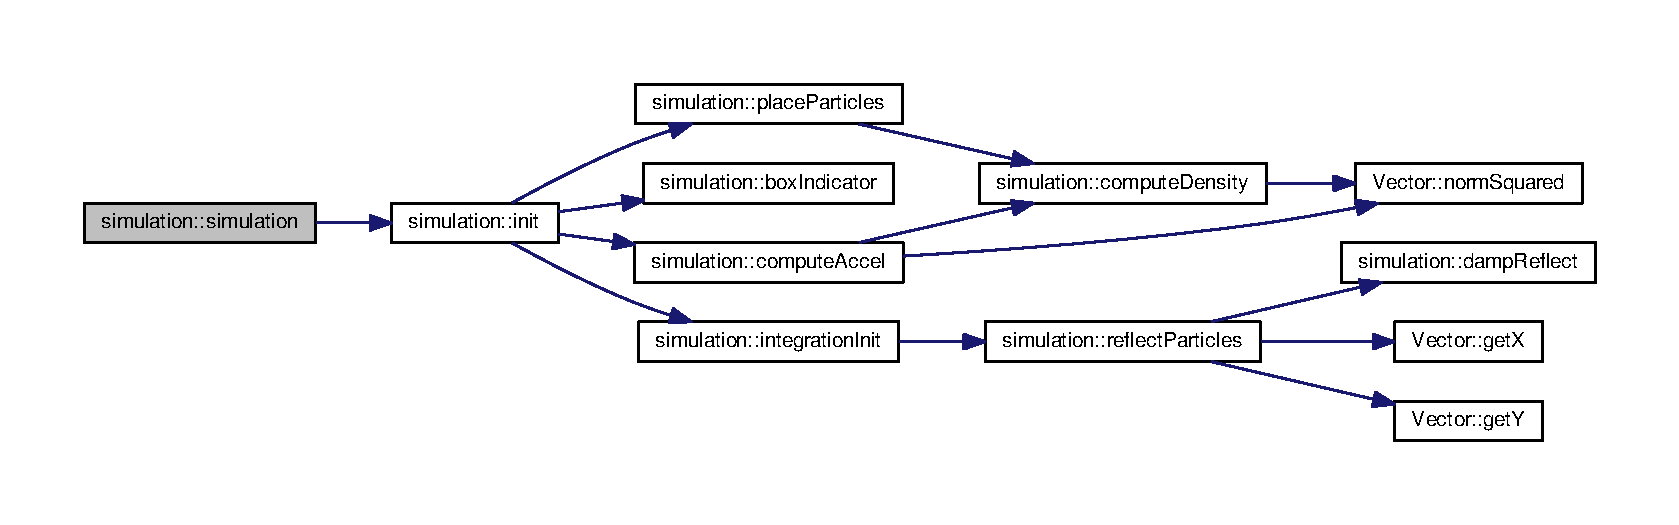
\includegraphics[width=350pt]{classsimulation_a30fdcc611ae9a656a3aebb8445e4607d_cgraph}
\end{center}
\end{figure}




\subsection{Dokumentacja funkcji składowych}
\hypertarget{classsimulation_acd02ace3dc0db98c4c85cba7d75fa46e}{\index{simulation@{simulation}!box\-Indicator@{box\-Indicator}}
\index{box\-Indicator@{box\-Indicator}!simulation@{simulation}}
\subsubsection[{box\-Indicator}]{\setlength{\rightskip}{0pt plus 5cm}bool simulation\-::box\-Indicator (
\begin{DoxyParamCaption}
\item[{float}]{x, }
\item[{float}]{y}
\end{DoxyParamCaption}
)}}\label{classsimulation_acd02ace3dc0db98c4c85cba7d75fa46e}
sprawdza przynależność punku do obszaru początkowego -\/ prostokąta 
\begin{DoxyParams}[1]{Parametry}
\mbox{\tt in}  & {\em x} & -\/ pierwsza współrzędna \\
\hline
\mbox{\tt in}  & {\em y} & -\/ druga współrzędna \\
\hline
\end{DoxyParams}
\begin{DoxyReturn}{Zwraca}
true jeśli warunek spełniony 
\end{DoxyReturn}


Definicja w linii 139 pliku simulation.\-cpp.



Oto graf wywoływań tej funkcji\-:\nopagebreak
\begin{figure}[H]
\begin{center}
\leavevmode
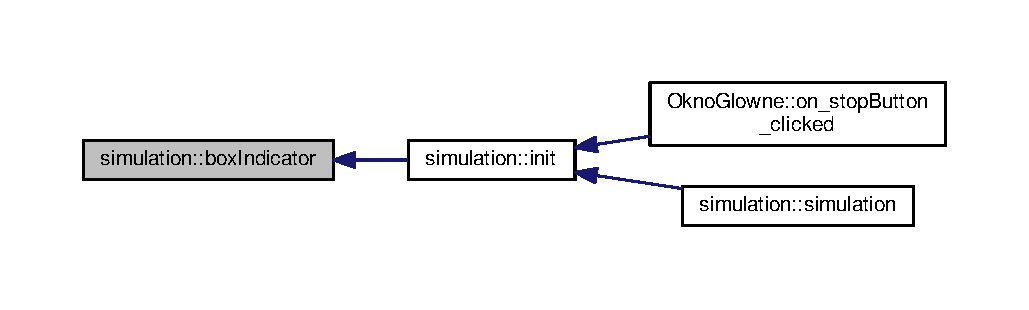
\includegraphics[width=350pt]{classsimulation_acd02ace3dc0db98c4c85cba7d75fa46e_icgraph}
\end{center}
\end{figure}


\hypertarget{classsimulation_a3c90f4d96f7cfbafc0ef8caf4927ae2d}{\index{simulation@{simulation}!circle\-Indicator@{circle\-Indicator}}
\index{circle\-Indicator@{circle\-Indicator}!simulation@{simulation}}
\subsubsection[{circle\-Indicator}]{\setlength{\rightskip}{0pt plus 5cm}bool simulation\-::circle\-Indicator (
\begin{DoxyParamCaption}
\item[{float}]{x, }
\item[{float}]{y}
\end{DoxyParamCaption}
)}}\label{classsimulation_a3c90f4d96f7cfbafc0ef8caf4927ae2d}
sprawdza przynależność punku do obszaru początkowego -\/ zewnętrza ćwierci okręgu 
\begin{DoxyParams}[1]{Parametry}
\mbox{\tt in}  & {\em x} & -\/ pierwsza współrzędna \\
\hline
\mbox{\tt in}  & {\em y} & -\/ druga współrzędna \\
\hline
\end{DoxyParams}
\begin{DoxyReturn}{Zwraca}
true jeśli warunek spełniony 
\end{DoxyReturn}


Definicja w linii 143 pliku simulation.\-cpp.

\hypertarget{classsimulation_a16b945b81e27680a709fffd8663bf856}{\index{simulation@{simulation}!compute\-Accel@{compute\-Accel}}
\index{compute\-Accel@{compute\-Accel}!simulation@{simulation}}
\subsubsection[{compute\-Accel}]{\setlength{\rightskip}{0pt plus 5cm}void simulation\-::compute\-Accel (
\begin{DoxyParamCaption}
\item[{{\bf params\-\_\-t} $\ast$}]{params}
\end{DoxyParamCaption}
)}}\label{classsimulation_a16b945b81e27680a709fffd8663bf856}
Implementuje formułę\-: \[ a_i = \frac{1}{\rho_i}\sum_{j\in N_i} f^{interact}_{ij} + g. \] która pozwala przybliżyć wartość przyspieszenia każdej cząstki jako sumę wektorów oddziaływań między wszystkimi cząsteczkami i wektora grawitacji \begin{DoxyNote}{Nota}
wektor grawitacji może ulegać zmianie podczas trwania symulacji 
\end{DoxyNote}


Definicja w linii 61 pliku simulation.\-cpp.



Oto graf wywołań dla tej funkcji\-:\nopagebreak
\begin{figure}[H]
\begin{center}
\leavevmode
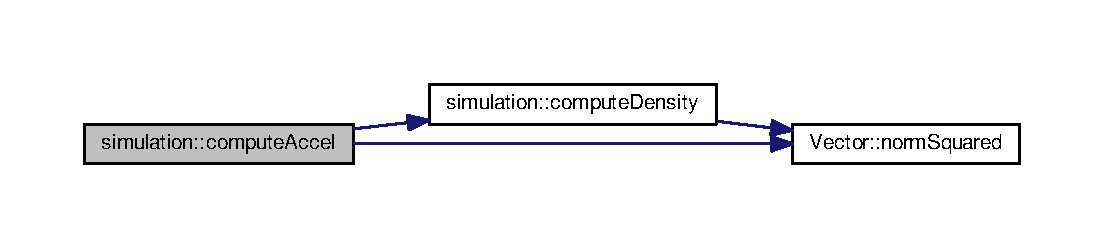
\includegraphics[width=350pt]{classsimulation_a16b945b81e27680a709fffd8663bf856_cgraph}
\end{center}
\end{figure}




Oto graf wywoływań tej funkcji\-:\nopagebreak
\begin{figure}[H]
\begin{center}
\leavevmode
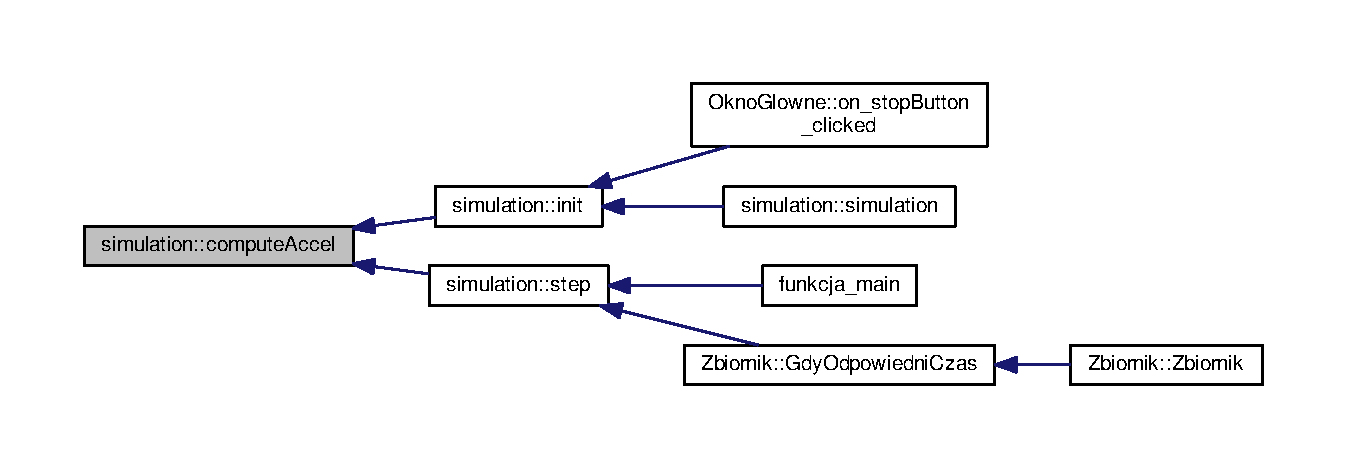
\includegraphics[width=350pt]{classsimulation_a16b945b81e27680a709fffd8663bf856_icgraph}
\end{center}
\end{figure}


\hypertarget{classsimulation_a7679fcd9a25d6cb5597338d054a30684}{\index{simulation@{simulation}!compute\-Density@{compute\-Density}}
\index{compute\-Density@{compute\-Density}!simulation@{simulation}}
\subsubsection[{compute\-Density}]{\setlength{\rightskip}{0pt plus 5cm}void simulation\-::compute\-Density (
\begin{DoxyParamCaption}
\item[{{\bf params\-\_\-t} $\ast$}]{\-\_\-p}
\end{DoxyParamCaption}
)}}\label{classsimulation_a7679fcd9a25d6cb5597338d054a30684}
Implementuje formułę\-: \[ \rho_i = \frac{4m}{\pi h^8}\sum_{j\in N_i} (h^2-r^2)^3, \] która pozwala przybliżyć wartość gęstości w miejscu i-\/tej cząstki na podstawie jej oddziaływań ze wszystkimi innymi cząstkami w zbiorniku. \begin{DoxyNote}{Nota}
wartość ciśnienia zawizualizować można kolorem cząstki. 
\end{DoxyNote}


Definicja w linii 40 pliku simulation.\-cpp.



Oto graf wywołań dla tej funkcji\-:\nopagebreak
\begin{figure}[H]
\begin{center}
\leavevmode
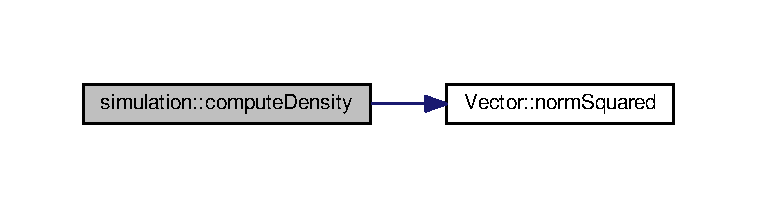
\includegraphics[width=350pt]{classsimulation_a7679fcd9a25d6cb5597338d054a30684_cgraph}
\end{center}
\end{figure}




Oto graf wywoływań tej funkcji\-:\nopagebreak
\begin{figure}[H]
\begin{center}
\leavevmode
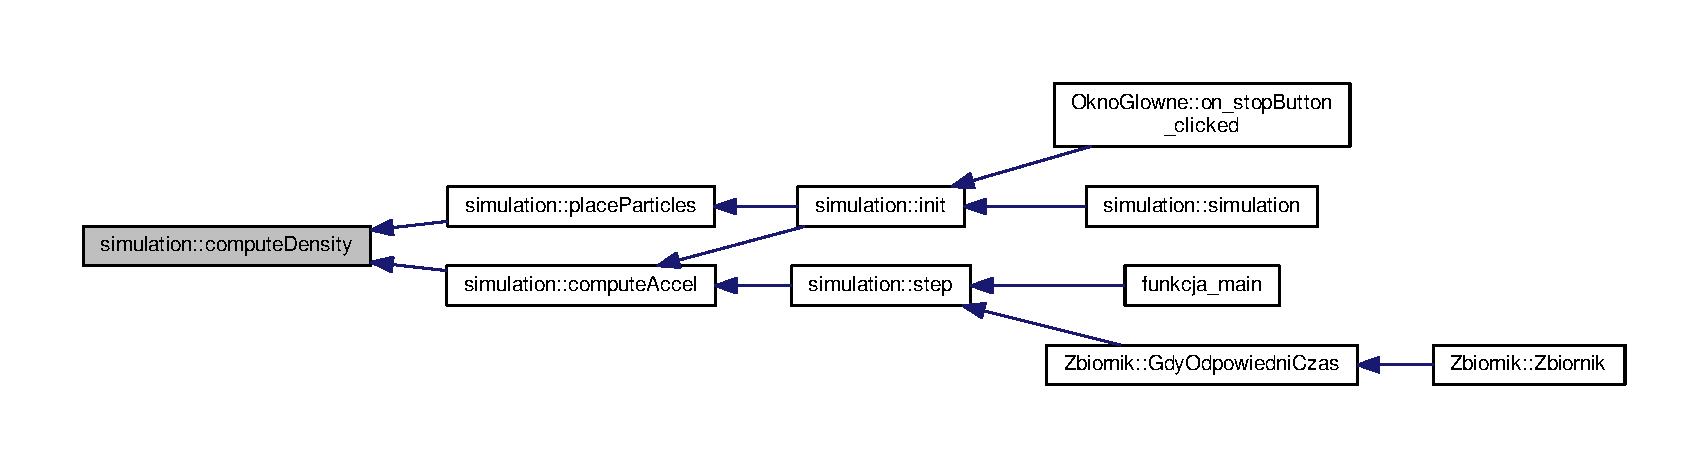
\includegraphics[width=350pt]{classsimulation_a7679fcd9a25d6cb5597338d054a30684_icgraph}
\end{center}
\end{figure}


\hypertarget{classsimulation_a353d4dd3a66197360e882bc29a6fef0b}{\index{simulation@{simulation}!damp\-Reflect@{damp\-Reflect}}
\index{damp\-Reflect@{damp\-Reflect}!simulation@{simulation}}
\subsubsection[{damp\-Reflect}]{\setlength{\rightskip}{0pt plus 5cm}void simulation\-::damp\-Reflect (
\begin{DoxyParamCaption}
\item[{float}]{\-\_\-barrier, }
\item[{unsigned}]{i, }
\item[{float \&(Vector\-::$\ast$)()}]{getter}
\end{DoxyParamCaption}
)}}\label{classsimulation_a353d4dd3a66197360e882bc29a6fef0b}
odpowiednio modyfikuje położenie cząstki oraz zmniejsza wartości prędkości i ich zwroty 
\begin{DoxyParams}[1]{Parametry}
\mbox{\tt in}  & {\em \-\_\-barrier} & -\/ odpowiednia współrzędna krawędzi \\
\hline
\mbox{\tt in}  & {\em i} & -\/ numer cząstki \\
\hline
\mbox{\tt in}  & {\em getter} & -\/ wskaźnik na metodę wybierającą odpowiednią współrzędną z Vectora \\
\hline
\end{DoxyParams}


Definicja w linii 100 pliku simulation.\-cpp.



Oto graf wywoływań tej funkcji\-:\nopagebreak
\begin{figure}[H]
\begin{center}
\leavevmode
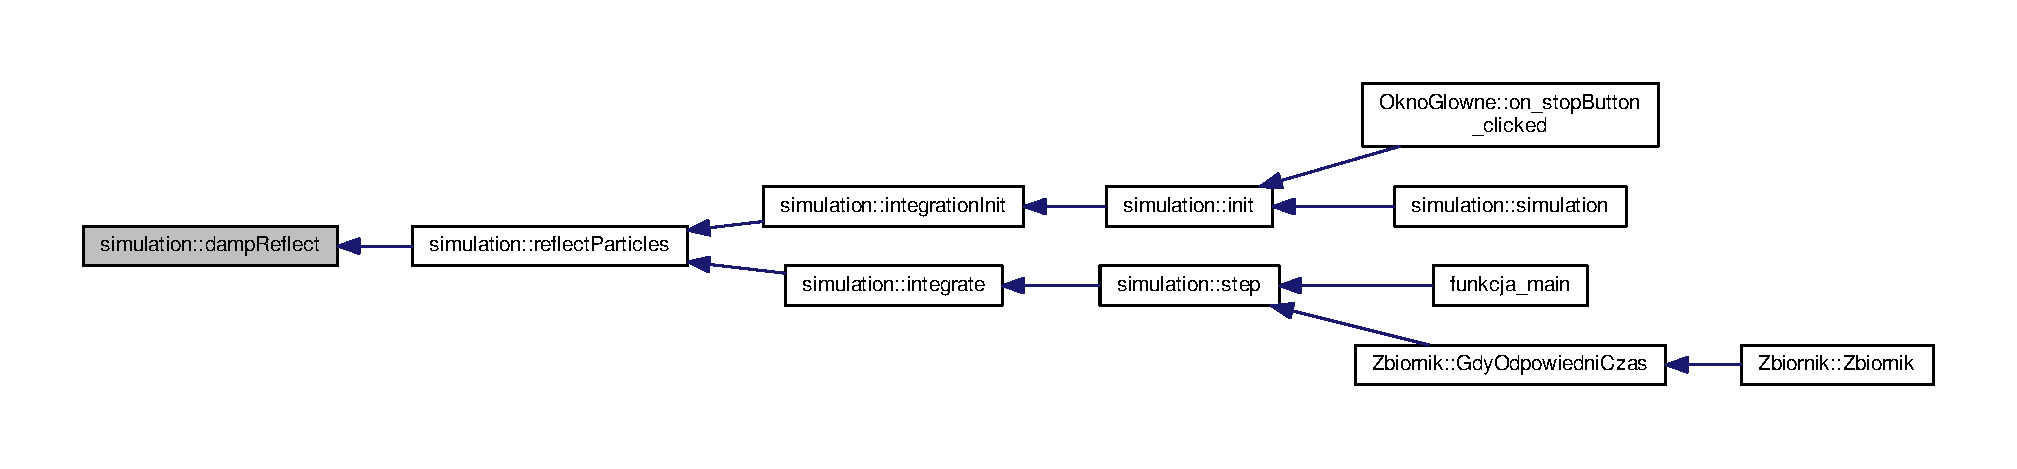
\includegraphics[width=350pt]{classsimulation_a353d4dd3a66197360e882bc29a6fef0b_icgraph}
\end{center}
\end{figure}


\hypertarget{classsimulation_abe09252527aa58fbec8144063be3e950}{\index{simulation@{simulation}!get\-N@{get\-N}}
\index{get\-N@{get\-N}!simulation@{simulation}}
\subsubsection[{get\-N}]{\setlength{\rightskip}{0pt plus 5cm}const unsigned\& simulation\-::get\-N (
\begin{DoxyParamCaption}
{}
\end{DoxyParamCaption}
) const\hspace{0.3cm}{\ttfamily [inline]}}}\label{classsimulation_abe09252527aa58fbec8144063be3e950}
zwraca liczbę cząstek użytych do symulacji \begin{DoxyReturn}{Zwraca}
liczba cząstek 
\end{DoxyReturn}


Definicja w linii 196 pliku simulation.\-hh.



Oto graf wywoływań tej funkcji\-:\nopagebreak
\begin{figure}[H]
\begin{center}
\leavevmode
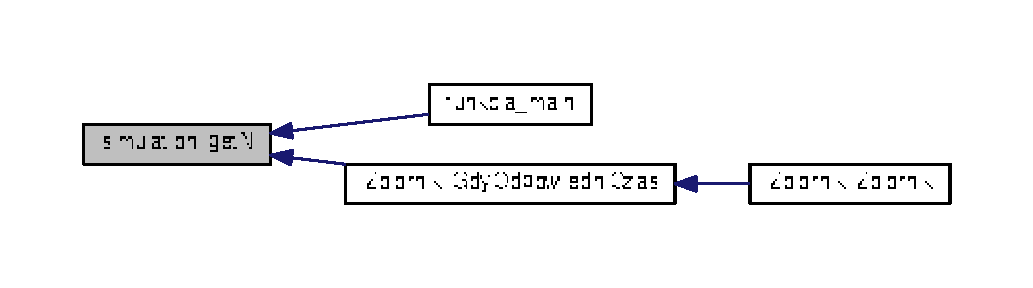
\includegraphics[width=350pt]{classsimulation_abe09252527aa58fbec8144063be3e950_icgraph}
\end{center}
\end{figure}


\hypertarget{classsimulation_a2e12616e089dd7f9742c25933bf630ef}{\index{simulation@{simulation}!init@{init}}
\index{init@{init}!simulation@{simulation}}
\subsubsection[{init}]{\setlength{\rightskip}{0pt plus 5cm}void simulation\-::init (
\begin{DoxyParamCaption}
{}
\end{DoxyParamCaption}
)}}\label{classsimulation_a2e12616e089dd7f9742c25933bf630ef}
dodaje cząstki do symulacji i określa ich początkowe parametry dynamiczne 

Definicja w linii 171 pliku simulation.\-cpp.



Oto graf wywołań dla tej funkcji\-:\nopagebreak
\begin{figure}[H]
\begin{center}
\leavevmode
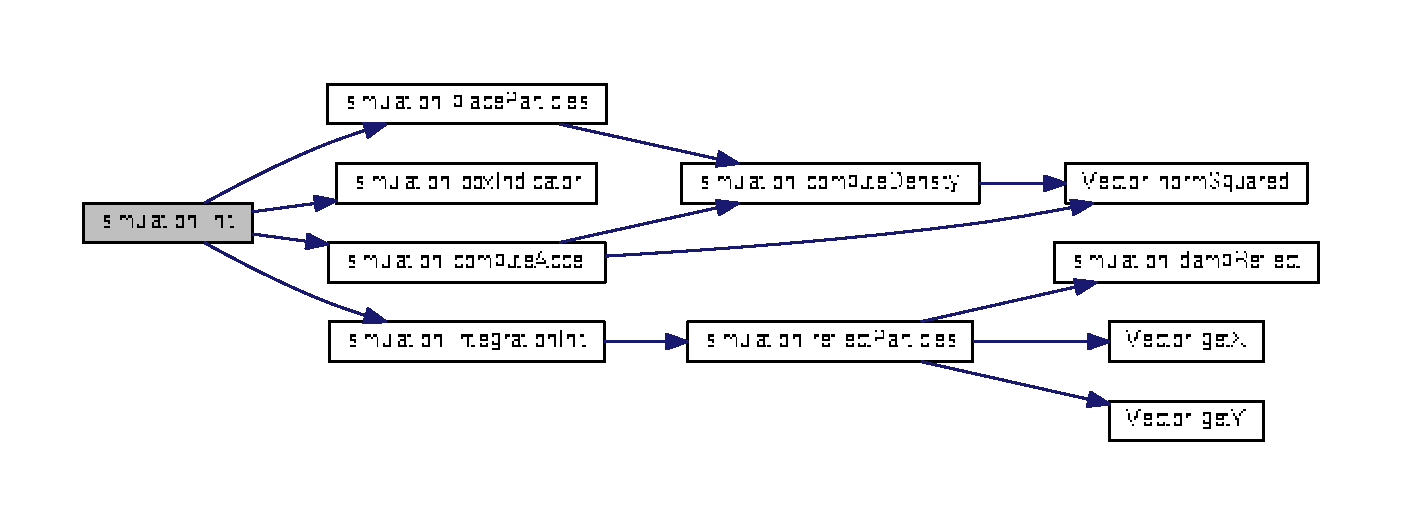
\includegraphics[width=350pt]{classsimulation_a2e12616e089dd7f9742c25933bf630ef_cgraph}
\end{center}
\end{figure}




Oto graf wywoływań tej funkcji\-:\nopagebreak
\begin{figure}[H]
\begin{center}
\leavevmode
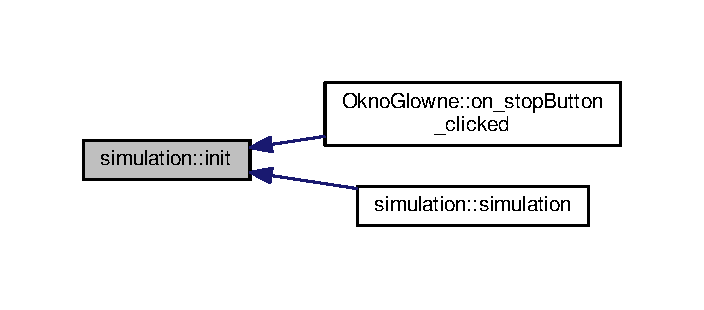
\includegraphics[width=338pt]{classsimulation_a2e12616e089dd7f9742c25933bf630ef_icgraph}
\end{center}
\end{figure}


\hypertarget{classsimulation_a2b1ca39aee7b85ac2babecfd2784c459}{\index{simulation@{simulation}!integrate@{integrate}}
\index{integrate@{integrate}!simulation@{simulation}}
\subsubsection[{integrate}]{\setlength{\rightskip}{0pt plus 5cm}void simulation\-::integrate (
\begin{DoxyParamCaption}
\item[{float}]{dt}
\end{DoxyParamCaption}
)}}\label{classsimulation_a2b1ca39aee7b85ac2babecfd2784c459}
odpowiada za realizację ruchu symulowanych cząstek 
\begin{DoxyParams}[1]{Parametry}
\mbox{\tt in}  & {\em dt} & -\/ wartość skoku czasu symulacji \\
\hline
\end{DoxyParams}


Definicja w linii 130 pliku simulation.\-cpp.



Oto graf wywołań dla tej funkcji\-:\nopagebreak
\begin{figure}[H]
\begin{center}
\leavevmode
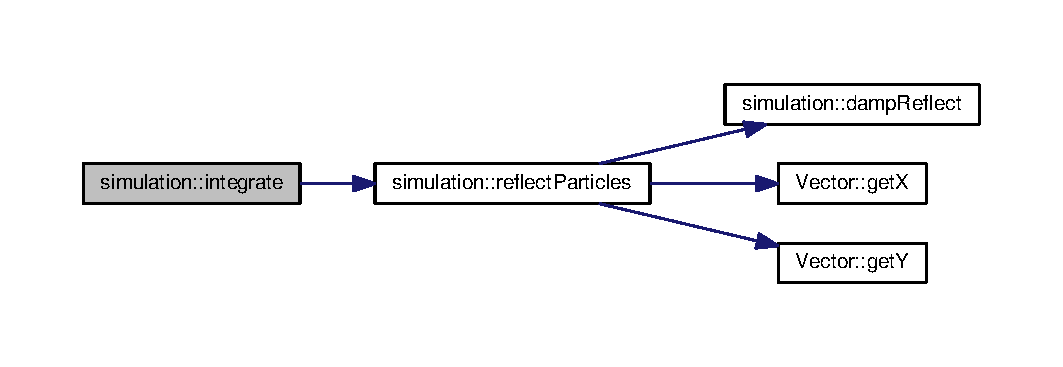
\includegraphics[width=350pt]{classsimulation_a2b1ca39aee7b85ac2babecfd2784c459_cgraph}
\end{center}
\end{figure}




Oto graf wywoływań tej funkcji\-:\nopagebreak
\begin{figure}[H]
\begin{center}
\leavevmode
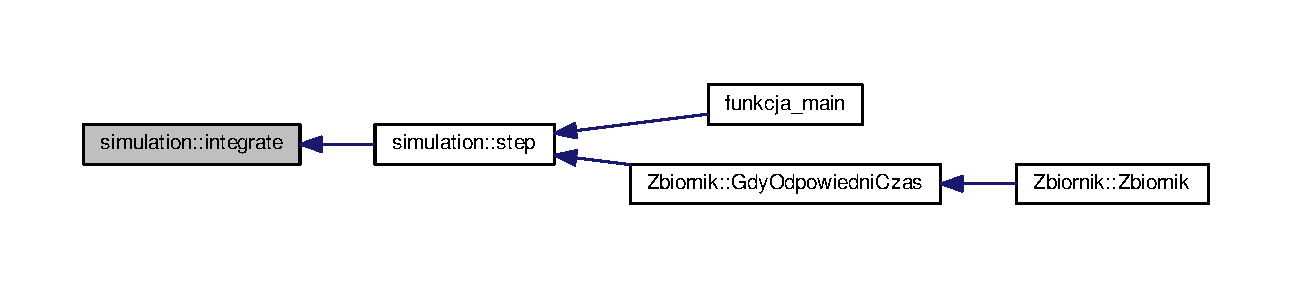
\includegraphics[width=350pt]{classsimulation_a2b1ca39aee7b85ac2babecfd2784c459_icgraph}
\end{center}
\end{figure}


\hypertarget{classsimulation_a300e67649652f2ae9337af3d5244e0f7}{\index{simulation@{simulation}!integration\-Init@{integration\-Init}}
\index{integration\-Init@{integration\-Init}!simulation@{simulation}}
\subsubsection[{integration\-Init}]{\setlength{\rightskip}{0pt plus 5cm}void simulation\-::integration\-Init (
\begin{DoxyParamCaption}
\item[{float}]{dt}
\end{DoxyParamCaption}
)}}\label{classsimulation_a300e67649652f2ae9337af3d5244e0f7}
zadaje początkowe parametry dynamiczne cząstek 
\begin{DoxyParams}[1]{Parametry}
\mbox{\tt in}  & {\em dt} & -\/ wartość skoku czasu symulacji \\
\hline
\end{DoxyParams}


Definicja w linii 122 pliku simulation.\-cpp.



Oto graf wywołań dla tej funkcji\-:\nopagebreak
\begin{figure}[H]
\begin{center}
\leavevmode
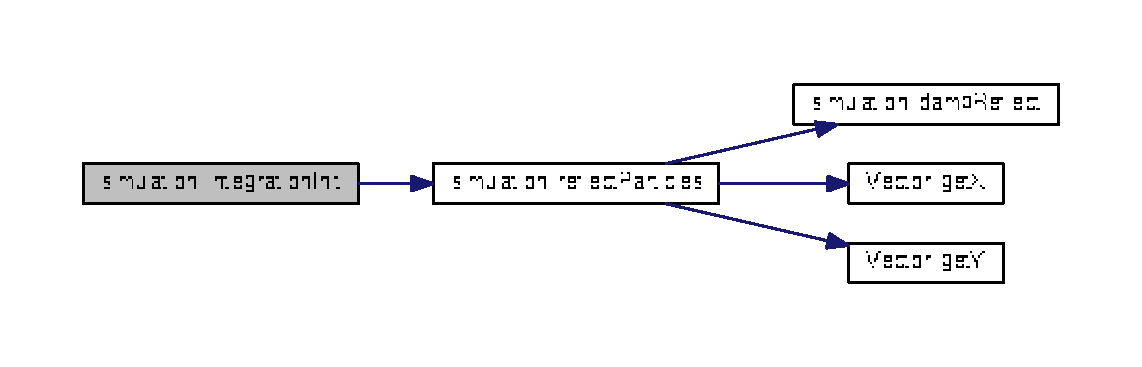
\includegraphics[width=350pt]{classsimulation_a300e67649652f2ae9337af3d5244e0f7_cgraph}
\end{center}
\end{figure}




Oto graf wywoływań tej funkcji\-:\nopagebreak
\begin{figure}[H]
\begin{center}
\leavevmode
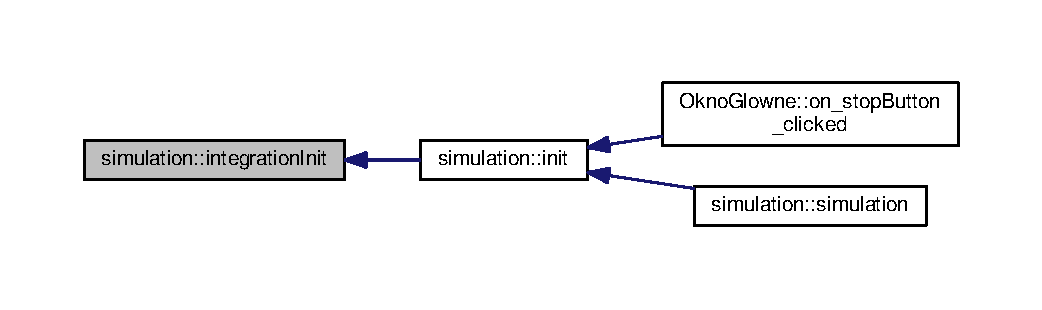
\includegraphics[width=350pt]{classsimulation_a300e67649652f2ae9337af3d5244e0f7_icgraph}
\end{center}
\end{figure}


\hypertarget{classsimulation_a33ce66b2291920bd1ba29889ff7c0c75}{\index{simulation@{simulation}!place\-Particles@{place\-Particles}}
\index{place\-Particles@{place\-Particles}!simulation@{simulation}}
\subsubsection[{place\-Particles}]{\setlength{\rightskip}{0pt plus 5cm}{\bf simulation} \& simulation\-::place\-Particles (
\begin{DoxyParamCaption}
\item[{{\bf params\-\_\-t} $\ast$}]{params, }
\item[{bool(simulation\-::$\ast$)(float x, float y)}]{container\-Indicator}
\end{DoxyParamCaption}
)}}\label{classsimulation_a33ce66b2291920bd1ba29889ff7c0c75}
iteruje po siatce punktów wewnątrz zbiornika i dodaje do symulacji te, dla których warunek określony przez funkcję container\-Indicator jest spełniony 
\begin{DoxyParams}[1]{Parametry}
\mbox{\tt in}  & {\em params} & -\/ parametry symulacji \\
\hline
\mbox{\tt in}  & {\em container\-Indicator} & -\/ warunek przynależności do obszaru \\
\hline
\end{DoxyParams}


Definicja w linii 147 pliku simulation.\-cpp.



Oto graf wywołań dla tej funkcji\-:\nopagebreak
\begin{figure}[H]
\begin{center}
\leavevmode
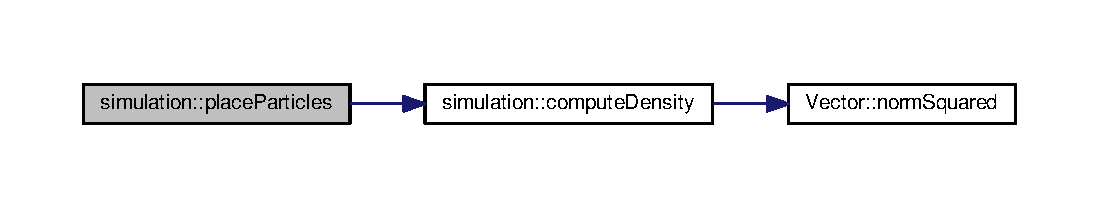
\includegraphics[width=350pt]{classsimulation_a33ce66b2291920bd1ba29889ff7c0c75_cgraph}
\end{center}
\end{figure}




Oto graf wywoływań tej funkcji\-:\nopagebreak
\begin{figure}[H]
\begin{center}
\leavevmode
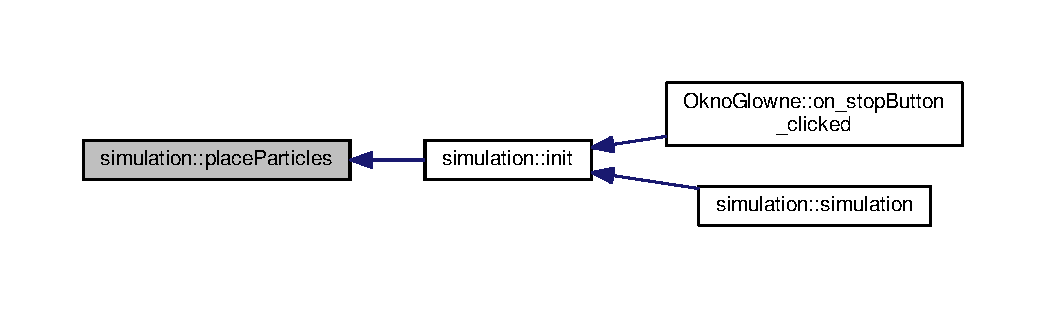
\includegraphics[width=350pt]{classsimulation_a33ce66b2291920bd1ba29889ff7c0c75_icgraph}
\end{center}
\end{figure}


\hypertarget{classsimulation_a9cb3fe3f985ceb039736a666923a20b5}{\index{simulation@{simulation}!reflect\-Particles@{reflect\-Particles}}
\index{reflect\-Particles@{reflect\-Particles}!simulation@{simulation}}
\subsubsection[{reflect\-Particles}]{\setlength{\rightskip}{0pt plus 5cm}void simulation\-::reflect\-Particles (
\begin{DoxyParamCaption}
{}
\end{DoxyParamCaption}
)}}\label{classsimulation_a9cb3fe3f985ceb039736a666923a20b5}
po wykryciu kolizji wywołuje damp\-Reflect z odpowiednimi parametrami 

Definicja w linii 112 pliku simulation.\-cpp.



Oto graf wywołań dla tej funkcji\-:\nopagebreak
\begin{figure}[H]
\begin{center}
\leavevmode
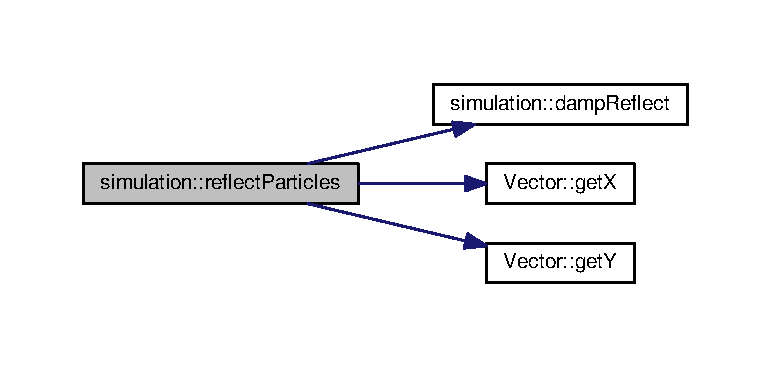
\includegraphics[width=350pt]{classsimulation_a9cb3fe3f985ceb039736a666923a20b5_cgraph}
\end{center}
\end{figure}




Oto graf wywoływań tej funkcji\-:\nopagebreak
\begin{figure}[H]
\begin{center}
\leavevmode
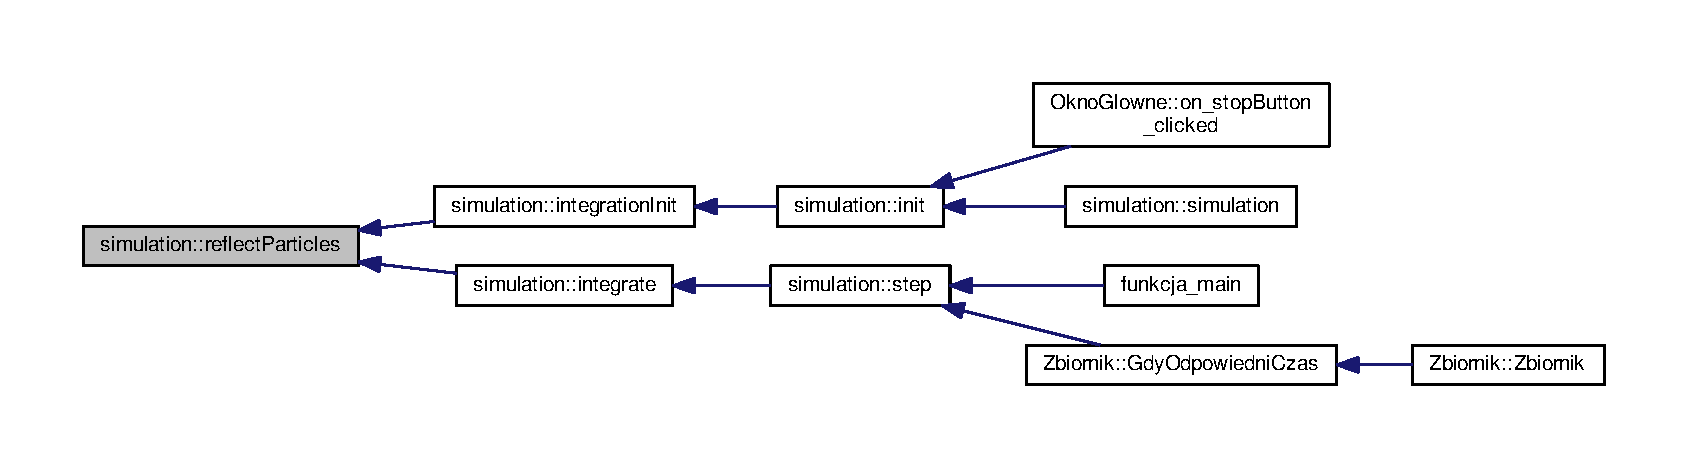
\includegraphics[width=350pt]{classsimulation_a9cb3fe3f985ceb039736a666923a20b5_icgraph}
\end{center}
\end{figure}


\hypertarget{classsimulation_a111e26e535d53ced834dbd52948b5d69}{\index{simulation@{simulation}!step@{step}}
\index{step@{step}!simulation@{simulation}}
\subsubsection[{step}]{\setlength{\rightskip}{0pt plus 5cm}void simulation\-::step (
\begin{DoxyParamCaption}
{}
\end{DoxyParamCaption}
)}}\label{classsimulation_a111e26e535d53ced834dbd52948b5d69}
odpowiada za realizację ruchu symulowanych cząstek 

Definicja w linii 180 pliku simulation.\-cpp.



Oto graf wywołań dla tej funkcji\-:\nopagebreak
\begin{figure}[H]
\begin{center}
\leavevmode
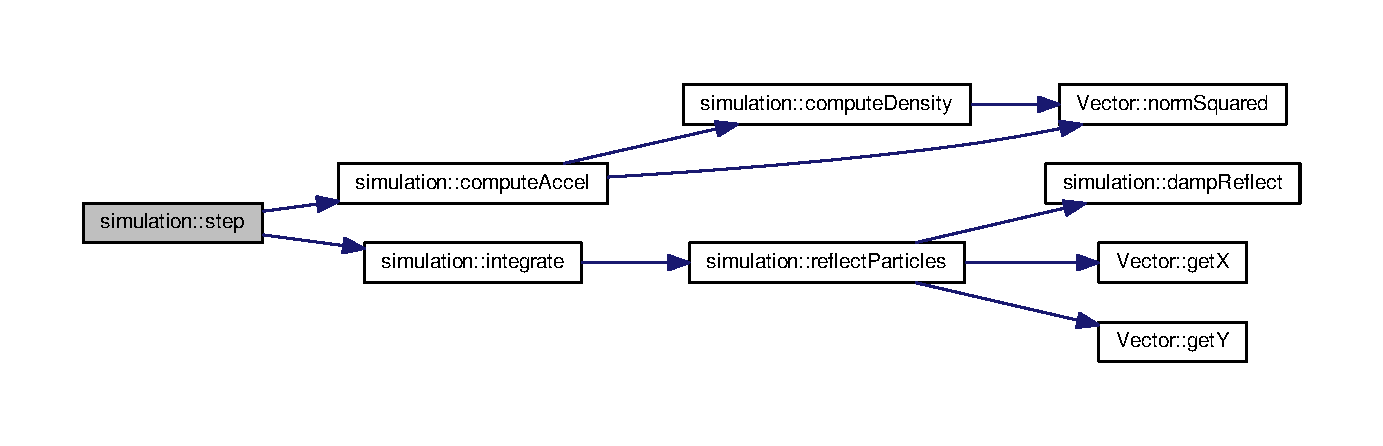
\includegraphics[width=350pt]{classsimulation_a111e26e535d53ced834dbd52948b5d69_cgraph}
\end{center}
\end{figure}




Oto graf wywoływań tej funkcji\-:\nopagebreak
\begin{figure}[H]
\begin{center}
\leavevmode
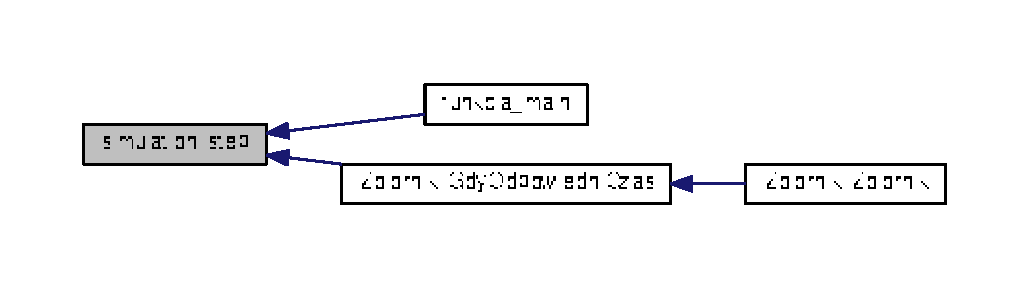
\includegraphics[width=350pt]{classsimulation_a111e26e535d53ced834dbd52948b5d69_icgraph}
\end{center}
\end{figure}




\subsection{Dokumentacja przyjaciół i funkcji związanych}
\hypertarget{classsimulation_a1f6414b078a2823f5cea77fc1235e1d9}{\index{simulation@{simulation}!operator$<$$<$@{operator$<$$<$}}
\index{operator$<$$<$@{operator$<$$<$}!simulation@{simulation}}
\subsubsection[{operator$<$$<$}]{\setlength{\rightskip}{0pt plus 5cm}std\-::ostream\& operator$<$$<$ (
\begin{DoxyParamCaption}
\item[{std\-::ostream \&}]{\-\_\-os, }
\item[{const {\bf simulation} \&}]{\-\_\-s}
\end{DoxyParamCaption}
)\hspace{0.3cm}{\ttfamily [friend]}}}\label{classsimulation_a1f6414b078a2823f5cea77fc1235e1d9}


Definicja w linii 190 pliku simulation.\-cpp.

\hypertarget{classsimulation_a444a8643309d19294860a4ae144137fe}{\index{simulation@{simulation}!Zbiornik@{Zbiornik}}
\index{Zbiornik@{Zbiornik}!simulation@{simulation}}
\subsubsection[{Zbiornik}]{\setlength{\rightskip}{0pt plus 5cm}friend class {\bf Zbiornik}\hspace{0.3cm}{\ttfamily [friend]}}}\label{classsimulation_a444a8643309d19294860a4ae144137fe}


Definicja w linii 64 pliku simulation.\-hh.



\subsection{Dokumentacja atrybutów składowych}
\hypertarget{classsimulation_a7b5ca0e5fc096989be7966a73c360b7f}{\index{simulation@{simulation}!a@{a}}
\index{a@{a}!simulation@{simulation}}
\subsubsection[{a}]{\setlength{\rightskip}{0pt plus 5cm}{\bf Vector}$\ast$ simulation\-::a\hspace{0.3cm}{\ttfamily [private]}}}\label{classsimulation_a7b5ca0e5fc096989be7966a73c360b7f}


Definicja w linii 71 pliku simulation.\-hh.

\hypertarget{classsimulation_a22eb97765a5c60adf3d995f7a110da70}{\index{simulation@{simulation}!n@{n}}
\index{n@{n}!simulation@{simulation}}
\subsubsection[{n}]{\setlength{\rightskip}{0pt plus 5cm}unsigned simulation\-::n\hspace{0.3cm}{\ttfamily [private]}}}\label{classsimulation_a22eb97765a5c60adf3d995f7a110da70}


Definicja w linii 66 pliku simulation.\-hh.

\hypertarget{classsimulation_a5412fd01febe99f12ae38e30eb692ff0}{\index{simulation@{simulation}!p@{p}}
\index{p@{p}!simulation@{simulation}}
\subsubsection[{p}]{\setlength{\rightskip}{0pt plus 5cm}{\bf Vector}$\ast$ simulation\-::p\hspace{0.3cm}{\ttfamily [private]}}}\label{classsimulation_a5412fd01febe99f12ae38e30eb692ff0}


Definicja w linii 68 pliku simulation.\-hh.

\hypertarget{classsimulation_a861b82cc3c0e7e58abfba464a133dae3}{\index{simulation@{simulation}!params@{params}}
\index{params@{params}!simulation@{simulation}}
\subsubsection[{params}]{\setlength{\rightskip}{0pt plus 5cm}{\bf params\-\_\-t}$\ast$ simulation\-::params}}\label{classsimulation_a861b82cc3c0e7e58abfba464a133dae3}


Definicja w linii 75 pliku simulation.\-hh.

\hypertarget{classsimulation_a44081d4edd92e17a3e1067b976031a00}{\index{simulation@{simulation}!rho@{rho}}
\index{rho@{rho}!simulation@{simulation}}
\subsubsection[{rho}]{\setlength{\rightskip}{0pt plus 5cm}float$\ast$ simulation\-::rho\hspace{0.3cm}{\ttfamily [private]}}}\label{classsimulation_a44081d4edd92e17a3e1067b976031a00}


Definicja w linii 67 pliku simulation.\-hh.

\hypertarget{classsimulation_a39dbad79b1b8667840638a35e839a3f7}{\index{simulation@{simulation}!v@{v}}
\index{v@{v}!simulation@{simulation}}
\subsubsection[{v}]{\setlength{\rightskip}{0pt plus 5cm}{\bf Vector}$\ast$ simulation\-::v\hspace{0.3cm}{\ttfamily [private]}}}\label{classsimulation_a39dbad79b1b8667840638a35e839a3f7}


Definicja w linii 70 pliku simulation.\-hh.

\hypertarget{classsimulation_ae6da1f15728f49be7b0793700866ede9}{\index{simulation@{simulation}!vh@{vh}}
\index{vh@{vh}!simulation@{simulation}}
\subsubsection[{vh}]{\setlength{\rightskip}{0pt plus 5cm}{\bf Vector}$\ast$ simulation\-::vh\hspace{0.3cm}{\ttfamily [private]}}}\label{classsimulation_ae6da1f15728f49be7b0793700866ede9}


Definicja w linii 69 pliku simulation.\-hh.



Dokumentacja dla tej klasy została wygenerowana z plików\-:\begin{DoxyCompactItemize}
\item 
\hyperlink{simulation_8hh}{simulation.\-hh}\item 
\hyperlink{simulation_8cpp}{simulation.\-cpp}\end{DoxyCompactItemize}

\input{structstate__t}
\hypertarget{class_ui___d_main_window}{}\section{Dokumentacja klasy Ui\+\_\+\+D\+Main\+Window}
\label{class_ui___d_main_window}\index{Ui\+\_\+\+D\+Main\+Window@{Ui\+\_\+\+D\+Main\+Window}}


{\ttfamily \#include $<$ui\+\_\+dmainwindow.\+h$>$}



Diagram dziedziczenia dla Ui\+\_\+\+D\+Main\+Window
\nopagebreak
\begin{figure}[H]
\begin{center}
\leavevmode
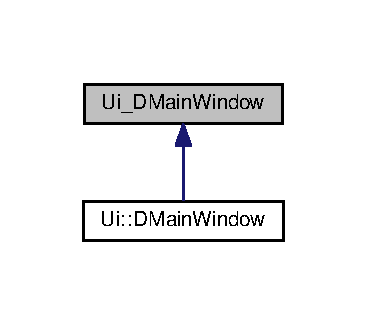
\includegraphics[width=181pt]{class_ui___d_main_window__inherit__graph}
\end{center}
\end{figure}
\subsection*{Metody publiczne}
\begin{DoxyCompactItemize}
\item 
void \hyperlink{class_ui___d_main_window_aa53f3a89bf520704a3e79037df2fd451}{setup\+Ui} (Q\+Main\+Window $\ast$\hyperlink{class_d_main_window}{D\+Main\+Window})
\item 
void \hyperlink{class_ui___d_main_window_a406169c751ddfd205b89375c7542827c}{retranslate\+Ui} (Q\+Main\+Window $\ast$\hyperlink{class_d_main_window}{D\+Main\+Window})
\end{DoxyCompactItemize}
\subsection*{Atrybuty publiczne}
\begin{DoxyCompactItemize}
\item 
Q\+Action $\ast$ \hyperlink{class_ui___d_main_window_a7ab98279e07bdd724a091ea06012c87b}{action\+\_\+\+Save}
\item 
Q\+Action $\ast$ \hyperlink{class_ui___d_main_window_a00e6b795743b676bdf3ed853e91f7029}{action\+\_\+\+Exit}
\item 
Q\+Action $\ast$ \hyperlink{class_ui___d_main_window_ae1fa62a4d27fa0f4a5c63c7c60cfdad2}{action\+Exit}
\item 
Q\+Action $\ast$ \hyperlink{class_ui___d_main_window_a6cfb6311ca1dd6e247d80255e2667ba7}{action\+Play}
\item 
Q\+Widget $\ast$ \hyperlink{class_ui___d_main_window_a94cf40cb4e645cfa2e80f36ffbf5018e}{central\+Widget}
\item 
Q\+Widget $\ast$ \hyperlink{class_ui___d_main_window_a777a56f3b74aa5b5cd5ff2c62a2968a9}{horizontal\+Layout\+Widget}
\item 
Q\+H\+Box\+Layout $\ast$ \hyperlink{class_ui___d_main_window_a4ab6ff85d8c5edef531b3f2111a04157}{horizontal\+Layout}
\item 
Q\+Push\+Button $\ast$ \hyperlink{class_ui___d_main_window_ad87cbf39ac14374923ed2a2b11e8b1bf}{play\+Button}
\item 
Q\+Push\+Button $\ast$ \hyperlink{class_ui___d_main_window_a70e142e35db4995a1fefa082406bdef3}{pause\+Button}
\item 
Q\+Push\+Button $\ast$ \hyperlink{class_ui___d_main_window_a1fe7797fff349a0f0d47d90c8438f386}{stop\+Button}
\item 
Q\+Slider $\ast$ \hyperlink{class_ui___d_main_window_a8d12f07935a52a597e57eddf50e5c98f}{slider\+Szybkosc\+Sym}
\item 
Q\+L\+C\+D\+Number $\ast$ \hyperlink{class_ui___d_main_window_a4eb8e2a87080f4f314eb96c52a82e39d}{lcd\+Szybkosc\+Sym}
\item 
Q\+Line\+Edit $\ast$ \hyperlink{class_ui___d_main_window_a73bafa5343a8e3cb7cd673a24be76008}{line\+Szybkosc\+Sym}
\item 
Q\+Line\+Edit $\ast$ \hyperlink{class_ui___d_main_window_aad165daf4686baecb2ccd6709c629579}{line\+Czas\+Sym}
\item 
Q\+L\+C\+D\+Number $\ast$ \hyperlink{class_ui___d_main_window_af49335a21dc17e53674f8b62a640ca2d}{lcd\+Czas\+Sym}
\item 
Q\+Line\+Edit $\ast$ \hyperlink{class_ui___d_main_window_a49c95cda7e035087a4367514e5540298}{line\+Liczba\+Czasteczek}
\item 
Q\+L\+C\+D\+Number $\ast$ \hyperlink{class_ui___d_main_window_a3d6afe29d882b3a9119b68d79c9b5e0f}{lcd\+Liczba\+Czasteczek}
\item 
Q\+Menu\+Bar $\ast$ \hyperlink{class_ui___d_main_window_a788ef749d82ca070e467e55cca0d47dd}{menu\+Bar}
\item 
Q\+Menu $\ast$ \hyperlink{class_ui___d_main_window_a991f4d15852faf04d8c12694b3e077ad}{menu\+\_\+\+File}
\item 
Q\+Menu $\ast$ \hyperlink{class_ui___d_main_window_a8826a3e34a5aa75fca2b8e45b7010a8b}{menu\+\_\+\+Edit}
\item 
Q\+Menu $\ast$ \hyperlink{class_ui___d_main_window_ac2997077098614d72b21d29c7a48350c}{menu\+\_\+\+Help}
\item 
Q\+Tool\+Bar $\ast$ \hyperlink{class_ui___d_main_window_a2e1da3781ee1e5913b25b85f4c29b97f}{main\+Tool\+Bar}
\item 
Q\+Status\+Bar $\ast$ \hyperlink{class_ui___d_main_window_ac9e025e7279839dd7ab1686456d1ae21}{status\+Bar}
\item 
Q\+Tool\+Bar $\ast$ \hyperlink{class_ui___d_main_window_abba1dae1dd835c7a7dd39da623cd4580}{tool\+Bar}
\end{DoxyCompactItemize}


\subsection{Opis szczegółowy}


Definicja w linii 31 pliku ui\+\_\+dmainwindow.\+h.



\subsection{Dokumentacja funkcji składowych}
\hypertarget{class_ui___d_main_window_a406169c751ddfd205b89375c7542827c}{}\index{Ui\+\_\+\+D\+Main\+Window@{Ui\+\_\+\+D\+Main\+Window}!retranslate\+Ui@{retranslate\+Ui}}
\index{retranslate\+Ui@{retranslate\+Ui}!Ui\+\_\+\+D\+Main\+Window@{Ui\+\_\+\+D\+Main\+Window}}
\subsubsection[{retranslate\+Ui}]{\setlength{\rightskip}{0pt plus 5cm}void Ui\+\_\+\+D\+Main\+Window\+::retranslate\+Ui (
\begin{DoxyParamCaption}
\item[{Q\+Main\+Window $\ast$}]{D\+Main\+Window}
\end{DoxyParamCaption}
)\hspace{0.3cm}{\ttfamily [inline]}}\label{class_ui___d_main_window_a406169c751ddfd205b89375c7542827c}


Definicja w linii 151 pliku ui\+\_\+dmainwindow.\+h.



Oto graf wywoływań tej funkcji\+:
\nopagebreak
\begin{figure}[H]
\begin{center}
\leavevmode
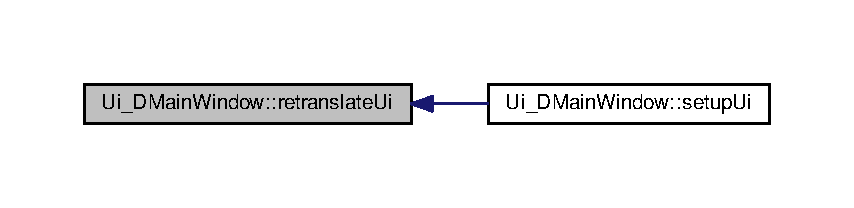
\includegraphics[width=350pt]{class_ui___d_main_window_a406169c751ddfd205b89375c7542827c_icgraph}
\end{center}
\end{figure}


\hypertarget{class_ui___d_main_window_aa53f3a89bf520704a3e79037df2fd451}{}\index{Ui\+\_\+\+D\+Main\+Window@{Ui\+\_\+\+D\+Main\+Window}!setup\+Ui@{setup\+Ui}}
\index{setup\+Ui@{setup\+Ui}!Ui\+\_\+\+D\+Main\+Window@{Ui\+\_\+\+D\+Main\+Window}}
\subsubsection[{setup\+Ui}]{\setlength{\rightskip}{0pt plus 5cm}void Ui\+\_\+\+D\+Main\+Window\+::setup\+Ui (
\begin{DoxyParamCaption}
\item[{Q\+Main\+Window $\ast$}]{D\+Main\+Window}
\end{DoxyParamCaption}
)\hspace{0.3cm}{\ttfamily [inline]}}\label{class_ui___d_main_window_aa53f3a89bf520704a3e79037df2fd451}


Definicja w linii 59 pliku ui\+\_\+dmainwindow.\+h.



Oto graf wywołań dla tej funkcji\+:
\nopagebreak
\begin{figure}[H]
\begin{center}
\leavevmode
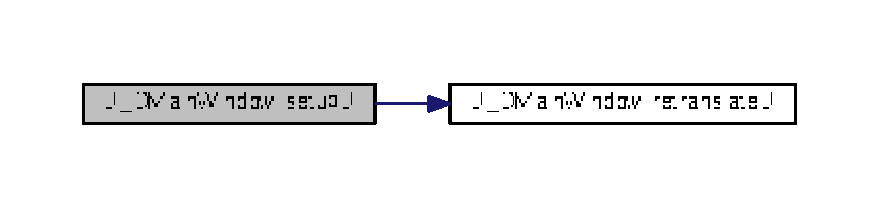
\includegraphics[width=350pt]{class_ui___d_main_window_aa53f3a89bf520704a3e79037df2fd451_cgraph}
\end{center}
\end{figure}




Oto graf wywoływań tej funkcji\+:
\nopagebreak
\begin{figure}[H]
\begin{center}
\leavevmode
\includegraphics[width=350pt]{class_ui___d_main_window_aa53f3a89bf520704a3e79037df2fd451_icgraph}
\end{center}
\end{figure}




\subsection{Dokumentacja atrybutów składowych}
\hypertarget{class_ui___d_main_window_a00e6b795743b676bdf3ed853e91f7029}{}\index{Ui\+\_\+\+D\+Main\+Window@{Ui\+\_\+\+D\+Main\+Window}!action\+\_\+\+Exit@{action\+\_\+\+Exit}}
\index{action\+\_\+\+Exit@{action\+\_\+\+Exit}!Ui\+\_\+\+D\+Main\+Window@{Ui\+\_\+\+D\+Main\+Window}}
\subsubsection[{action\+\_\+\+Exit}]{\setlength{\rightskip}{0pt plus 5cm}Q\+Action$\ast$ Ui\+\_\+\+D\+Main\+Window\+::action\+\_\+\+Exit}\label{class_ui___d_main_window_a00e6b795743b676bdf3ed853e91f7029}


Definicja w linii 35 pliku ui\+\_\+dmainwindow.\+h.

\hypertarget{class_ui___d_main_window_a7ab98279e07bdd724a091ea06012c87b}{}\index{Ui\+\_\+\+D\+Main\+Window@{Ui\+\_\+\+D\+Main\+Window}!action\+\_\+\+Save@{action\+\_\+\+Save}}
\index{action\+\_\+\+Save@{action\+\_\+\+Save}!Ui\+\_\+\+D\+Main\+Window@{Ui\+\_\+\+D\+Main\+Window}}
\subsubsection[{action\+\_\+\+Save}]{\setlength{\rightskip}{0pt plus 5cm}Q\+Action$\ast$ Ui\+\_\+\+D\+Main\+Window\+::action\+\_\+\+Save}\label{class_ui___d_main_window_a7ab98279e07bdd724a091ea06012c87b}


Definicja w linii 34 pliku ui\+\_\+dmainwindow.\+h.

\hypertarget{class_ui___d_main_window_ae1fa62a4d27fa0f4a5c63c7c60cfdad2}{}\index{Ui\+\_\+\+D\+Main\+Window@{Ui\+\_\+\+D\+Main\+Window}!action\+Exit@{action\+Exit}}
\index{action\+Exit@{action\+Exit}!Ui\+\_\+\+D\+Main\+Window@{Ui\+\_\+\+D\+Main\+Window}}
\subsubsection[{action\+Exit}]{\setlength{\rightskip}{0pt plus 5cm}Q\+Action$\ast$ Ui\+\_\+\+D\+Main\+Window\+::action\+Exit}\label{class_ui___d_main_window_ae1fa62a4d27fa0f4a5c63c7c60cfdad2}


Definicja w linii 36 pliku ui\+\_\+dmainwindow.\+h.

\hypertarget{class_ui___d_main_window_a6cfb6311ca1dd6e247d80255e2667ba7}{}\index{Ui\+\_\+\+D\+Main\+Window@{Ui\+\_\+\+D\+Main\+Window}!action\+Play@{action\+Play}}
\index{action\+Play@{action\+Play}!Ui\+\_\+\+D\+Main\+Window@{Ui\+\_\+\+D\+Main\+Window}}
\subsubsection[{action\+Play}]{\setlength{\rightskip}{0pt plus 5cm}Q\+Action$\ast$ Ui\+\_\+\+D\+Main\+Window\+::action\+Play}\label{class_ui___d_main_window_a6cfb6311ca1dd6e247d80255e2667ba7}


Definicja w linii 37 pliku ui\+\_\+dmainwindow.\+h.

\hypertarget{class_ui___d_main_window_a94cf40cb4e645cfa2e80f36ffbf5018e}{}\index{Ui\+\_\+\+D\+Main\+Window@{Ui\+\_\+\+D\+Main\+Window}!central\+Widget@{central\+Widget}}
\index{central\+Widget@{central\+Widget}!Ui\+\_\+\+D\+Main\+Window@{Ui\+\_\+\+D\+Main\+Window}}
\subsubsection[{central\+Widget}]{\setlength{\rightskip}{0pt plus 5cm}Q\+Widget$\ast$ Ui\+\_\+\+D\+Main\+Window\+::central\+Widget}\label{class_ui___d_main_window_a94cf40cb4e645cfa2e80f36ffbf5018e}


Definicja w linii 38 pliku ui\+\_\+dmainwindow.\+h.

\hypertarget{class_ui___d_main_window_a4ab6ff85d8c5edef531b3f2111a04157}{}\index{Ui\+\_\+\+D\+Main\+Window@{Ui\+\_\+\+D\+Main\+Window}!horizontal\+Layout@{horizontal\+Layout}}
\index{horizontal\+Layout@{horizontal\+Layout}!Ui\+\_\+\+D\+Main\+Window@{Ui\+\_\+\+D\+Main\+Window}}
\subsubsection[{horizontal\+Layout}]{\setlength{\rightskip}{0pt plus 5cm}Q\+H\+Box\+Layout$\ast$ Ui\+\_\+\+D\+Main\+Window\+::horizontal\+Layout}\label{class_ui___d_main_window_a4ab6ff85d8c5edef531b3f2111a04157}


Definicja w linii 40 pliku ui\+\_\+dmainwindow.\+h.

\hypertarget{class_ui___d_main_window_a777a56f3b74aa5b5cd5ff2c62a2968a9}{}\index{Ui\+\_\+\+D\+Main\+Window@{Ui\+\_\+\+D\+Main\+Window}!horizontal\+Layout\+Widget@{horizontal\+Layout\+Widget}}
\index{horizontal\+Layout\+Widget@{horizontal\+Layout\+Widget}!Ui\+\_\+\+D\+Main\+Window@{Ui\+\_\+\+D\+Main\+Window}}
\subsubsection[{horizontal\+Layout\+Widget}]{\setlength{\rightskip}{0pt plus 5cm}Q\+Widget$\ast$ Ui\+\_\+\+D\+Main\+Window\+::horizontal\+Layout\+Widget}\label{class_ui___d_main_window_a777a56f3b74aa5b5cd5ff2c62a2968a9}


Definicja w linii 39 pliku ui\+\_\+dmainwindow.\+h.

\hypertarget{class_ui___d_main_window_af49335a21dc17e53674f8b62a640ca2d}{}\index{Ui\+\_\+\+D\+Main\+Window@{Ui\+\_\+\+D\+Main\+Window}!lcd\+Czas\+Sym@{lcd\+Czas\+Sym}}
\index{lcd\+Czas\+Sym@{lcd\+Czas\+Sym}!Ui\+\_\+\+D\+Main\+Window@{Ui\+\_\+\+D\+Main\+Window}}
\subsubsection[{lcd\+Czas\+Sym}]{\setlength{\rightskip}{0pt plus 5cm}Q\+L\+C\+D\+Number$\ast$ Ui\+\_\+\+D\+Main\+Window\+::lcd\+Czas\+Sym}\label{class_ui___d_main_window_af49335a21dc17e53674f8b62a640ca2d}


Definicja w linii 48 pliku ui\+\_\+dmainwindow.\+h.

\hypertarget{class_ui___d_main_window_a3d6afe29d882b3a9119b68d79c9b5e0f}{}\index{Ui\+\_\+\+D\+Main\+Window@{Ui\+\_\+\+D\+Main\+Window}!lcd\+Liczba\+Czasteczek@{lcd\+Liczba\+Czasteczek}}
\index{lcd\+Liczba\+Czasteczek@{lcd\+Liczba\+Czasteczek}!Ui\+\_\+\+D\+Main\+Window@{Ui\+\_\+\+D\+Main\+Window}}
\subsubsection[{lcd\+Liczba\+Czasteczek}]{\setlength{\rightskip}{0pt plus 5cm}Q\+L\+C\+D\+Number$\ast$ Ui\+\_\+\+D\+Main\+Window\+::lcd\+Liczba\+Czasteczek}\label{class_ui___d_main_window_a3d6afe29d882b3a9119b68d79c9b5e0f}


Definicja w linii 50 pliku ui\+\_\+dmainwindow.\+h.

\hypertarget{class_ui___d_main_window_a4eb8e2a87080f4f314eb96c52a82e39d}{}\index{Ui\+\_\+\+D\+Main\+Window@{Ui\+\_\+\+D\+Main\+Window}!lcd\+Szybkosc\+Sym@{lcd\+Szybkosc\+Sym}}
\index{lcd\+Szybkosc\+Sym@{lcd\+Szybkosc\+Sym}!Ui\+\_\+\+D\+Main\+Window@{Ui\+\_\+\+D\+Main\+Window}}
\subsubsection[{lcd\+Szybkosc\+Sym}]{\setlength{\rightskip}{0pt plus 5cm}Q\+L\+C\+D\+Number$\ast$ Ui\+\_\+\+D\+Main\+Window\+::lcd\+Szybkosc\+Sym}\label{class_ui___d_main_window_a4eb8e2a87080f4f314eb96c52a82e39d}


Definicja w linii 45 pliku ui\+\_\+dmainwindow.\+h.

\hypertarget{class_ui___d_main_window_aad165daf4686baecb2ccd6709c629579}{}\index{Ui\+\_\+\+D\+Main\+Window@{Ui\+\_\+\+D\+Main\+Window}!line\+Czas\+Sym@{line\+Czas\+Sym}}
\index{line\+Czas\+Sym@{line\+Czas\+Sym}!Ui\+\_\+\+D\+Main\+Window@{Ui\+\_\+\+D\+Main\+Window}}
\subsubsection[{line\+Czas\+Sym}]{\setlength{\rightskip}{0pt plus 5cm}Q\+Line\+Edit$\ast$ Ui\+\_\+\+D\+Main\+Window\+::line\+Czas\+Sym}\label{class_ui___d_main_window_aad165daf4686baecb2ccd6709c629579}


Definicja w linii 47 pliku ui\+\_\+dmainwindow.\+h.

\hypertarget{class_ui___d_main_window_a49c95cda7e035087a4367514e5540298}{}\index{Ui\+\_\+\+D\+Main\+Window@{Ui\+\_\+\+D\+Main\+Window}!line\+Liczba\+Czasteczek@{line\+Liczba\+Czasteczek}}
\index{line\+Liczba\+Czasteczek@{line\+Liczba\+Czasteczek}!Ui\+\_\+\+D\+Main\+Window@{Ui\+\_\+\+D\+Main\+Window}}
\subsubsection[{line\+Liczba\+Czasteczek}]{\setlength{\rightskip}{0pt plus 5cm}Q\+Line\+Edit$\ast$ Ui\+\_\+\+D\+Main\+Window\+::line\+Liczba\+Czasteczek}\label{class_ui___d_main_window_a49c95cda7e035087a4367514e5540298}


Definicja w linii 49 pliku ui\+\_\+dmainwindow.\+h.

\hypertarget{class_ui___d_main_window_a73bafa5343a8e3cb7cd673a24be76008}{}\index{Ui\+\_\+\+D\+Main\+Window@{Ui\+\_\+\+D\+Main\+Window}!line\+Szybkosc\+Sym@{line\+Szybkosc\+Sym}}
\index{line\+Szybkosc\+Sym@{line\+Szybkosc\+Sym}!Ui\+\_\+\+D\+Main\+Window@{Ui\+\_\+\+D\+Main\+Window}}
\subsubsection[{line\+Szybkosc\+Sym}]{\setlength{\rightskip}{0pt plus 5cm}Q\+Line\+Edit$\ast$ Ui\+\_\+\+D\+Main\+Window\+::line\+Szybkosc\+Sym}\label{class_ui___d_main_window_a73bafa5343a8e3cb7cd673a24be76008}


Definicja w linii 46 pliku ui\+\_\+dmainwindow.\+h.

\hypertarget{class_ui___d_main_window_a2e1da3781ee1e5913b25b85f4c29b97f}{}\index{Ui\+\_\+\+D\+Main\+Window@{Ui\+\_\+\+D\+Main\+Window}!main\+Tool\+Bar@{main\+Tool\+Bar}}
\index{main\+Tool\+Bar@{main\+Tool\+Bar}!Ui\+\_\+\+D\+Main\+Window@{Ui\+\_\+\+D\+Main\+Window}}
\subsubsection[{main\+Tool\+Bar}]{\setlength{\rightskip}{0pt plus 5cm}Q\+Tool\+Bar$\ast$ Ui\+\_\+\+D\+Main\+Window\+::main\+Tool\+Bar}\label{class_ui___d_main_window_a2e1da3781ee1e5913b25b85f4c29b97f}


Definicja w linii 55 pliku ui\+\_\+dmainwindow.\+h.

\hypertarget{class_ui___d_main_window_a8826a3e34a5aa75fca2b8e45b7010a8b}{}\index{Ui\+\_\+\+D\+Main\+Window@{Ui\+\_\+\+D\+Main\+Window}!menu\+\_\+\+Edit@{menu\+\_\+\+Edit}}
\index{menu\+\_\+\+Edit@{menu\+\_\+\+Edit}!Ui\+\_\+\+D\+Main\+Window@{Ui\+\_\+\+D\+Main\+Window}}
\subsubsection[{menu\+\_\+\+Edit}]{\setlength{\rightskip}{0pt plus 5cm}Q\+Menu$\ast$ Ui\+\_\+\+D\+Main\+Window\+::menu\+\_\+\+Edit}\label{class_ui___d_main_window_a8826a3e34a5aa75fca2b8e45b7010a8b}


Definicja w linii 53 pliku ui\+\_\+dmainwindow.\+h.

\hypertarget{class_ui___d_main_window_a991f4d15852faf04d8c12694b3e077ad}{}\index{Ui\+\_\+\+D\+Main\+Window@{Ui\+\_\+\+D\+Main\+Window}!menu\+\_\+\+File@{menu\+\_\+\+File}}
\index{menu\+\_\+\+File@{menu\+\_\+\+File}!Ui\+\_\+\+D\+Main\+Window@{Ui\+\_\+\+D\+Main\+Window}}
\subsubsection[{menu\+\_\+\+File}]{\setlength{\rightskip}{0pt plus 5cm}Q\+Menu$\ast$ Ui\+\_\+\+D\+Main\+Window\+::menu\+\_\+\+File}\label{class_ui___d_main_window_a991f4d15852faf04d8c12694b3e077ad}


Definicja w linii 52 pliku ui\+\_\+dmainwindow.\+h.

\hypertarget{class_ui___d_main_window_ac2997077098614d72b21d29c7a48350c}{}\index{Ui\+\_\+\+D\+Main\+Window@{Ui\+\_\+\+D\+Main\+Window}!menu\+\_\+\+Help@{menu\+\_\+\+Help}}
\index{menu\+\_\+\+Help@{menu\+\_\+\+Help}!Ui\+\_\+\+D\+Main\+Window@{Ui\+\_\+\+D\+Main\+Window}}
\subsubsection[{menu\+\_\+\+Help}]{\setlength{\rightskip}{0pt plus 5cm}Q\+Menu$\ast$ Ui\+\_\+\+D\+Main\+Window\+::menu\+\_\+\+Help}\label{class_ui___d_main_window_ac2997077098614d72b21d29c7a48350c}


Definicja w linii 54 pliku ui\+\_\+dmainwindow.\+h.

\hypertarget{class_ui___d_main_window_a788ef749d82ca070e467e55cca0d47dd}{}\index{Ui\+\_\+\+D\+Main\+Window@{Ui\+\_\+\+D\+Main\+Window}!menu\+Bar@{menu\+Bar}}
\index{menu\+Bar@{menu\+Bar}!Ui\+\_\+\+D\+Main\+Window@{Ui\+\_\+\+D\+Main\+Window}}
\subsubsection[{menu\+Bar}]{\setlength{\rightskip}{0pt plus 5cm}Q\+Menu\+Bar$\ast$ Ui\+\_\+\+D\+Main\+Window\+::menu\+Bar}\label{class_ui___d_main_window_a788ef749d82ca070e467e55cca0d47dd}


Definicja w linii 51 pliku ui\+\_\+dmainwindow.\+h.

\hypertarget{class_ui___d_main_window_a70e142e35db4995a1fefa082406bdef3}{}\index{Ui\+\_\+\+D\+Main\+Window@{Ui\+\_\+\+D\+Main\+Window}!pause\+Button@{pause\+Button}}
\index{pause\+Button@{pause\+Button}!Ui\+\_\+\+D\+Main\+Window@{Ui\+\_\+\+D\+Main\+Window}}
\subsubsection[{pause\+Button}]{\setlength{\rightskip}{0pt plus 5cm}Q\+Push\+Button$\ast$ Ui\+\_\+\+D\+Main\+Window\+::pause\+Button}\label{class_ui___d_main_window_a70e142e35db4995a1fefa082406bdef3}


Definicja w linii 42 pliku ui\+\_\+dmainwindow.\+h.

\hypertarget{class_ui___d_main_window_ad87cbf39ac14374923ed2a2b11e8b1bf}{}\index{Ui\+\_\+\+D\+Main\+Window@{Ui\+\_\+\+D\+Main\+Window}!play\+Button@{play\+Button}}
\index{play\+Button@{play\+Button}!Ui\+\_\+\+D\+Main\+Window@{Ui\+\_\+\+D\+Main\+Window}}
\subsubsection[{play\+Button}]{\setlength{\rightskip}{0pt plus 5cm}Q\+Push\+Button$\ast$ Ui\+\_\+\+D\+Main\+Window\+::play\+Button}\label{class_ui___d_main_window_ad87cbf39ac14374923ed2a2b11e8b1bf}


Definicja w linii 41 pliku ui\+\_\+dmainwindow.\+h.

\hypertarget{class_ui___d_main_window_a8d12f07935a52a597e57eddf50e5c98f}{}\index{Ui\+\_\+\+D\+Main\+Window@{Ui\+\_\+\+D\+Main\+Window}!slider\+Szybkosc\+Sym@{slider\+Szybkosc\+Sym}}
\index{slider\+Szybkosc\+Sym@{slider\+Szybkosc\+Sym}!Ui\+\_\+\+D\+Main\+Window@{Ui\+\_\+\+D\+Main\+Window}}
\subsubsection[{slider\+Szybkosc\+Sym}]{\setlength{\rightskip}{0pt plus 5cm}Q\+Slider$\ast$ Ui\+\_\+\+D\+Main\+Window\+::slider\+Szybkosc\+Sym}\label{class_ui___d_main_window_a8d12f07935a52a597e57eddf50e5c98f}


Definicja w linii 44 pliku ui\+\_\+dmainwindow.\+h.

\hypertarget{class_ui___d_main_window_ac9e025e7279839dd7ab1686456d1ae21}{}\index{Ui\+\_\+\+D\+Main\+Window@{Ui\+\_\+\+D\+Main\+Window}!status\+Bar@{status\+Bar}}
\index{status\+Bar@{status\+Bar}!Ui\+\_\+\+D\+Main\+Window@{Ui\+\_\+\+D\+Main\+Window}}
\subsubsection[{status\+Bar}]{\setlength{\rightskip}{0pt plus 5cm}Q\+Status\+Bar$\ast$ Ui\+\_\+\+D\+Main\+Window\+::status\+Bar}\label{class_ui___d_main_window_ac9e025e7279839dd7ab1686456d1ae21}


Definicja w linii 56 pliku ui\+\_\+dmainwindow.\+h.

\hypertarget{class_ui___d_main_window_a1fe7797fff349a0f0d47d90c8438f386}{}\index{Ui\+\_\+\+D\+Main\+Window@{Ui\+\_\+\+D\+Main\+Window}!stop\+Button@{stop\+Button}}
\index{stop\+Button@{stop\+Button}!Ui\+\_\+\+D\+Main\+Window@{Ui\+\_\+\+D\+Main\+Window}}
\subsubsection[{stop\+Button}]{\setlength{\rightskip}{0pt plus 5cm}Q\+Push\+Button$\ast$ Ui\+\_\+\+D\+Main\+Window\+::stop\+Button}\label{class_ui___d_main_window_a1fe7797fff349a0f0d47d90c8438f386}


Definicja w linii 43 pliku ui\+\_\+dmainwindow.\+h.

\hypertarget{class_ui___d_main_window_abba1dae1dd835c7a7dd39da623cd4580}{}\index{Ui\+\_\+\+D\+Main\+Window@{Ui\+\_\+\+D\+Main\+Window}!tool\+Bar@{tool\+Bar}}
\index{tool\+Bar@{tool\+Bar}!Ui\+\_\+\+D\+Main\+Window@{Ui\+\_\+\+D\+Main\+Window}}
\subsubsection[{tool\+Bar}]{\setlength{\rightskip}{0pt plus 5cm}Q\+Tool\+Bar$\ast$ Ui\+\_\+\+D\+Main\+Window\+::tool\+Bar}\label{class_ui___d_main_window_abba1dae1dd835c7a7dd39da623cd4580}


Definicja w linii 57 pliku ui\+\_\+dmainwindow.\+h.



Dokumentacja dla tej klasy została wygenerowana z pliku\+:\begin{DoxyCompactItemize}
\item 
\hyperlink{ui__dmainwindow_8h}{ui\+\_\+dmainwindow.\+h}\end{DoxyCompactItemize}

\hypertarget{class_vector}{}\section{Dokumentacja klasy Vector}
\label{class_vector}\index{Vector@{Vector}}


klasa \hyperlink{class_vector}{Vector}  




{\ttfamily \#include $<$vector.\+hh$>$}

\subsection*{Metody publiczne}
\begin{DoxyCompactItemize}
\item 
\hyperlink{class_vector_af3c1b04bfbb10e29433842202365a6c4}{Vector} (float \+\_\+x=0, float \+\_\+y=0)
\begin{DoxyCompactList}\small\item\em Współrzędne wektora. \end{DoxyCompactList}\item 
float \hyperlink{class_vector_ab2878a1bb81982dc83363646e25ce665}{get\+X} () const 
\begin{DoxyCompactList}\small\item\em zwraga pierwszą współrzędną wektora \end{DoxyCompactList}\item 
float \hyperlink{class_vector_a86293fe7a035979fd252be6071488b6a}{get\+Y} () const 
\begin{DoxyCompactList}\small\item\em pobiera drugą współrzędną wektora \end{DoxyCompactList}\item 
float \& \hyperlink{class_vector_aeca06c929d4ab3078a828723a88621e6}{get\+X} ()
\begin{DoxyCompactList}\small\item\em pobiera pierwszą współrzędną wektora \end{DoxyCompactList}\item 
float \& \hyperlink{class_vector_ab0cc77ce300a60de0ab734555886ad5d}{get\+Y} ()
\begin{DoxyCompactList}\small\item\em pobiera drugą współrzędną wektora \end{DoxyCompactList}\item 
\hyperlink{class_vector}{Vector} \& \hyperlink{class_vector_a4eeab5be24ee846de3012e67a4e34820}{operator+=} (const \hyperlink{class_vector}{Vector} \&\+\_\+v)
\begin{DoxyCompactList}\small\item\em operator dodawania \end{DoxyCompactList}\item 
\hyperlink{class_vector}{Vector} \& \hyperlink{class_vector_aaaf87dbf15cd9492aa0c11874ae5afef}{operator-\/=} (const \hyperlink{class_vector}{Vector} \&\+\_\+v)
\begin{DoxyCompactList}\small\item\em operator odejmowania \end{DoxyCompactList}\item 
\hyperlink{class_vector}{Vector} \& \hyperlink{class_vector_a91ebac6d502ca1d54645e7c711549867}{operator$\ast$=} (const float \&\+\_\+c)
\begin{DoxyCompactList}\small\item\em operator skalowania \end{DoxyCompactList}\item 
\hyperlink{class_vector}{Vector} \hyperlink{class_vector_aa78eb4c9e5ac236c89f0853eefa347ac}{operator+} (const \hyperlink{class_vector}{Vector} \&\+\_\+v) const 
\begin{DoxyCompactList}\small\item\em operator dodawania \end{DoxyCompactList}\item 
\hyperlink{class_vector}{Vector} \hyperlink{class_vector_a94b6fde82bef6532c00358a0af448fc1}{operator-\/} (const \hyperlink{class_vector}{Vector} \&\+\_\+v) const 
\begin{DoxyCompactList}\small\item\em operator odejmowania \end{DoxyCompactList}\item 
\hyperlink{class_vector}{Vector} \hyperlink{class_vector_a8f0e64ee9a688803b1efce30fb0b2869}{operator$\ast$} (const float \&\+\_\+c) const 
\begin{DoxyCompactList}\small\item\em operator skalowania \end{DoxyCompactList}\item 
\hyperlink{class_vector}{Vector} \& \hyperlink{class_vector_ad44f6d9721d9584e7f847e449df73e11}{operator=} (const \hyperlink{class_vector}{Vector} \&\+\_\+v)
\begin{DoxyCompactList}\small\item\em operator przypisania \end{DoxyCompactList}\item 
float \hyperlink{class_vector_a18d3f2110be751ac3a658016bd3dca69}{norm\+Squared} ()
\begin{DoxyCompactList}\small\item\em kwadrat normy \end{DoxyCompactList}\end{DoxyCompactItemize}
\subsection*{Atrybuty prywatne}
\begin{DoxyCompactItemize}
\item 
float \hyperlink{class_vector_aca49165049a1e21ae47afcfc078819ed}{x}
\item 
float \hyperlink{class_vector_a81be9102fca6d9beea3efef522c4c09d}{y}
\end{DoxyCompactItemize}
\subsection*{Przyjaciele}
\begin{DoxyCompactItemize}
\item 
std\+::ostream \& \hyperlink{class_vector_a7973d0032b0df4c3ab89e1da167b86a9}{operator$<$$<$} (std\+::ostream \&\+\_\+os, const \hyperlink{class_vector}{Vector} \&\+\_\+s)
\end{DoxyCompactItemize}


\subsection{Opis szczegółowy}
Posiada metody do obsługi dwuelementowych wektorów o współrzędnych typu float 

Definicja w linii 10 pliku vector.\+hh.



\subsection{Dokumentacja konstruktora i destruktora}
\hypertarget{class_vector_af3c1b04bfbb10e29433842202365a6c4}{}\index{Vector@{Vector}!Vector@{Vector}}
\index{Vector@{Vector}!Vector@{Vector}}
\subsubsection[{Vector}]{\setlength{\rightskip}{0pt plus 5cm}Vector\+::\+Vector (
\begin{DoxyParamCaption}
\item[{float}]{\+\_\+x = {\ttfamily 0}, }
\item[{float}]{\+\_\+y = {\ttfamily 0}}
\end{DoxyParamCaption}
)\hspace{0.3cm}{\ttfamily [inline]}}\label{class_vector_af3c1b04bfbb10e29433842202365a6c4}
konstruktor wektora

Ustawia współrzędne wektora 
\begin{DoxyParams}[1]{Parametry}
\mbox{\tt in}  & {\em \+\_\+x} & -\/ pierwsza współrzędna (domyślnie\+: 0) \\
\hline
\mbox{\tt in}  & {\em \+\_\+y} & -\/ druga współrzędna (domyślnie\+: 0) \\
\hline
\end{DoxyParams}


Definicja w linii 22 pliku vector.\+hh.



Oto graf wywoływań tej funkcji\+:\nopagebreak
\begin{figure}[H]
\begin{center}
\leavevmode
\includegraphics[width=298pt]{class_vector_af3c1b04bfbb10e29433842202365a6c4_icgraph}
\end{center}
\end{figure}




\subsection{Dokumentacja funkcji składowych}
\hypertarget{class_vector_ab2878a1bb81982dc83363646e25ce665}{}\index{Vector@{Vector}!get\+X@{get\+X}}
\index{get\+X@{get\+X}!Vector@{Vector}}
\subsubsection[{get\+X}]{\setlength{\rightskip}{0pt plus 5cm}float Vector\+::get\+X (
\begin{DoxyParamCaption}
{}
\end{DoxyParamCaption}
) const\hspace{0.3cm}{\ttfamily [inline]}}\label{class_vector_ab2878a1bb81982dc83363646e25ce665}
\begin{DoxyReturn}{Zwraca}
pierwsza współrzędna wektora jako stała 
\end{DoxyReturn}


Definicja w linii 27 pliku vector.\+hh.



Oto graf wywoływań tej funkcji\+:\nopagebreak
\begin{figure}[H]
\begin{center}
\leavevmode
\includegraphics[width=350pt]{class_vector_ab2878a1bb81982dc83363646e25ce665_icgraph}
\end{center}
\end{figure}


\hypertarget{class_vector_aeca06c929d4ab3078a828723a88621e6}{}\index{Vector@{Vector}!get\+X@{get\+X}}
\index{get\+X@{get\+X}!Vector@{Vector}}
\subsubsection[{get\+X}]{\setlength{\rightskip}{0pt plus 5cm}float\& Vector\+::get\+X (
\begin{DoxyParamCaption}
{}
\end{DoxyParamCaption}
)\hspace{0.3cm}{\ttfamily [inline]}}\label{class_vector_aeca06c929d4ab3078a828723a88621e6}
\begin{DoxyReturn}{Zwraca}
pierwsza współrzędna wektora jako stała 
\end{DoxyReturn}


Definicja w linii 37 pliku vector.\+hh.

\hypertarget{class_vector_a86293fe7a035979fd252be6071488b6a}{}\index{Vector@{Vector}!get\+Y@{get\+Y}}
\index{get\+Y@{get\+Y}!Vector@{Vector}}
\subsubsection[{get\+Y}]{\setlength{\rightskip}{0pt plus 5cm}float Vector\+::get\+Y (
\begin{DoxyParamCaption}
{}
\end{DoxyParamCaption}
) const\hspace{0.3cm}{\ttfamily [inline]}}\label{class_vector_a86293fe7a035979fd252be6071488b6a}
\begin{DoxyReturn}{Zwraca}
druga współrzędna wektora jako stała 
\end{DoxyReturn}


Definicja w linii 32 pliku vector.\+hh.



Oto graf wywoływań tej funkcji\+:\nopagebreak
\begin{figure}[H]
\begin{center}
\leavevmode
\includegraphics[width=350pt]{class_vector_a86293fe7a035979fd252be6071488b6a_icgraph}
\end{center}
\end{figure}


\hypertarget{class_vector_ab0cc77ce300a60de0ab734555886ad5d}{}\index{Vector@{Vector}!get\+Y@{get\+Y}}
\index{get\+Y@{get\+Y}!Vector@{Vector}}
\subsubsection[{get\+Y}]{\setlength{\rightskip}{0pt plus 5cm}float\& Vector\+::get\+Y (
\begin{DoxyParamCaption}
{}
\end{DoxyParamCaption}
)\hspace{0.3cm}{\ttfamily [inline]}}\label{class_vector_ab0cc77ce300a60de0ab734555886ad5d}
\begin{DoxyReturn}{Zwraca}
druga współrzędna wektora jako stała 
\end{DoxyReturn}


Definicja w linii 42 pliku vector.\+hh.

\hypertarget{class_vector_a18d3f2110be751ac3a658016bd3dca69}{}\index{Vector@{Vector}!norm\+Squared@{norm\+Squared}}
\index{norm\+Squared@{norm\+Squared}!Vector@{Vector}}
\subsubsection[{norm\+Squared}]{\setlength{\rightskip}{0pt plus 5cm}float Vector\+::norm\+Squared (
\begin{DoxyParamCaption}
{}
\end{DoxyParamCaption}
)\hspace{0.3cm}{\ttfamily [inline]}}\label{class_vector_a18d3f2110be751ac3a658016bd3dca69}
Zwraca sumę kwadratów współrzędnych wektora \begin{DoxyReturn}{Zwraca}
wartość kwadratu normy 
\end{DoxyReturn}


Definicja w linii 105 pliku vector.\+hh.



Oto graf wywoływań tej funkcji\+:\nopagebreak
\begin{figure}[H]
\begin{center}
\leavevmode
\includegraphics[width=350pt]{class_vector_a18d3f2110be751ac3a658016bd3dca69_icgraph}
\end{center}
\end{figure}


\hypertarget{class_vector_a8f0e64ee9a688803b1efce30fb0b2869}{}\index{Vector@{Vector}!operator$\ast$@{operator$\ast$}}
\index{operator$\ast$@{operator$\ast$}!Vector@{Vector}}
\subsubsection[{operator$\ast$}]{\setlength{\rightskip}{0pt plus 5cm}{\bf Vector} Vector\+::operator$\ast$ (
\begin{DoxyParamCaption}
\item[{const float \&}]{\+\_\+c}
\end{DoxyParamCaption}
) const\hspace{0.3cm}{\ttfamily [inline]}}\label{class_vector_a8f0e64ee9a688803b1efce30fb0b2869}
Skaluje wektor 
\begin{DoxyParams}[1]{Parametry}
\mbox{\tt in}  & {\em \+\_\+c} & -\/ współczynnik skalowania \\
\hline
\end{DoxyParams}
\begin{DoxyReturn}{Zwraca}
przeskalowany wektor 
\end{DoxyReturn}


Definicja w linii 90 pliku vector.\+hh.



Oto graf wywołań dla tej funkcji\+:\nopagebreak
\begin{figure}[H]
\begin{center}
\leavevmode
\includegraphics[width=297pt]{class_vector_a8f0e64ee9a688803b1efce30fb0b2869_cgraph}
\end{center}
\end{figure}


\hypertarget{class_vector_a91ebac6d502ca1d54645e7c711549867}{}\index{Vector@{Vector}!operator$\ast$=@{operator$\ast$=}}
\index{operator$\ast$=@{operator$\ast$=}!Vector@{Vector}}
\subsubsection[{operator$\ast$=}]{\setlength{\rightskip}{0pt plus 5cm}{\bf Vector}\& Vector\+::operator$\ast$= (
\begin{DoxyParamCaption}
\item[{const float \&}]{\+\_\+c}
\end{DoxyParamCaption}
)\hspace{0.3cm}{\ttfamily [inline]}}\label{class_vector_a91ebac6d502ca1d54645e7c711549867}
Skaluje wektor 
\begin{DoxyParams}[1]{Parametry}
\mbox{\tt in}  & {\em \+\_\+c} & -\/ współczynnik \\
\hline
\end{DoxyParams}
\begin{DoxyReturn}{Zwraca}
referencja na pierwotny obiekt 
\end{DoxyReturn}


Definicja w linii 66 pliku vector.\+hh.

\hypertarget{class_vector_aa78eb4c9e5ac236c89f0853eefa347ac}{}\index{Vector@{Vector}!operator+@{operator+}}
\index{operator+@{operator+}!Vector@{Vector}}
\subsubsection[{operator+}]{\setlength{\rightskip}{0pt plus 5cm}{\bf Vector} Vector\+::operator+ (
\begin{DoxyParamCaption}
\item[{const {\bf Vector} \&}]{\+\_\+v}
\end{DoxyParamCaption}
) const\hspace{0.3cm}{\ttfamily [inline]}}\label{class_vector_aa78eb4c9e5ac236c89f0853eefa347ac}
Dodaje wartość dwóch wektorów 
\begin{DoxyParams}[1]{Parametry}
\mbox{\tt in}  & {\em \+\_\+v} & -\/ inny wektor \\
\hline
\end{DoxyParams}
\begin{DoxyReturn}{Zwraca}
wektor będący sumą 
\end{DoxyReturn}


Definicja w linii 74 pliku vector.\+hh.



Oto graf wywołań dla tej funkcji\+:\nopagebreak
\begin{figure}[H]
\begin{center}
\leavevmode
\includegraphics[width=298pt]{class_vector_aa78eb4c9e5ac236c89f0853eefa347ac_cgraph}
\end{center}
\end{figure}


\hypertarget{class_vector_a4eeab5be24ee846de3012e67a4e34820}{}\index{Vector@{Vector}!operator+=@{operator+=}}
\index{operator+=@{operator+=}!Vector@{Vector}}
\subsubsection[{operator+=}]{\setlength{\rightskip}{0pt plus 5cm}{\bf Vector}\& Vector\+::operator+= (
\begin{DoxyParamCaption}
\item[{const {\bf Vector} \&}]{\+\_\+v}
\end{DoxyParamCaption}
)\hspace{0.3cm}{\ttfamily [inline]}}\label{class_vector_a4eeab5be24ee846de3012e67a4e34820}
Dodaje wartość innego wektora do klasy 
\begin{DoxyParams}[1]{Parametry}
\mbox{\tt in}  & {\em \+\_\+v} & -\/ inny wektor \\
\hline
\end{DoxyParams}
\begin{DoxyReturn}{Zwraca}
referencja na pierwotny obiekt 
\end{DoxyReturn}


Definicja w linii 50 pliku vector.\+hh.

\hypertarget{class_vector_a94b6fde82bef6532c00358a0af448fc1}{}\index{Vector@{Vector}!operator-\/@{operator-\/}}
\index{operator-\/@{operator-\/}!Vector@{Vector}}
\subsubsection[{operator-\/}]{\setlength{\rightskip}{0pt plus 5cm}{\bf Vector} Vector\+::operator-\/ (
\begin{DoxyParamCaption}
\item[{const {\bf Vector} \&}]{\+\_\+v}
\end{DoxyParamCaption}
) const\hspace{0.3cm}{\ttfamily [inline]}}\label{class_vector_a94b6fde82bef6532c00358a0af448fc1}
Odejmuje wartość innego wektora od klasy 
\begin{DoxyParams}[1]{Parametry}
\mbox{\tt in}  & {\em \+\_\+v} & -\/ inny wektor \\
\hline
\end{DoxyParams}
\begin{DoxyReturn}{Zwraca}
wektor będący różnicą 
\end{DoxyReturn}


Definicja w linii 82 pliku vector.\+hh.



Oto graf wywołań dla tej funkcji\+:\nopagebreak
\begin{figure}[H]
\begin{center}
\leavevmode
\includegraphics[width=294pt]{class_vector_a94b6fde82bef6532c00358a0af448fc1_cgraph}
\end{center}
\end{figure}


\hypertarget{class_vector_aaaf87dbf15cd9492aa0c11874ae5afef}{}\index{Vector@{Vector}!operator-\/=@{operator-\/=}}
\index{operator-\/=@{operator-\/=}!Vector@{Vector}}
\subsubsection[{operator-\/=}]{\setlength{\rightskip}{0pt plus 5cm}{\bf Vector}\& Vector\+::operator-\/= (
\begin{DoxyParamCaption}
\item[{const {\bf Vector} \&}]{\+\_\+v}
\end{DoxyParamCaption}
)\hspace{0.3cm}{\ttfamily [inline]}}\label{class_vector_aaaf87dbf15cd9492aa0c11874ae5afef}
Odejmuje wartość innego wektora od klasy 
\begin{DoxyParams}[1]{Parametry}
\mbox{\tt in}  & {\em \+\_\+v} & -\/ inny wektor \\
\hline
\end{DoxyParams}
\begin{DoxyReturn}{Zwraca}
referencja na pierwotny obiekt 
\end{DoxyReturn}


Definicja w linii 58 pliku vector.\+hh.

\hypertarget{class_vector_ad44f6d9721d9584e7f847e449df73e11}{}\index{Vector@{Vector}!operator=@{operator=}}
\index{operator=@{operator=}!Vector@{Vector}}
\subsubsection[{operator=}]{\setlength{\rightskip}{0pt plus 5cm}{\bf Vector}\& Vector\+::operator= (
\begin{DoxyParamCaption}
\item[{const {\bf Vector} \&}]{\+\_\+v}
\end{DoxyParamCaption}
)\hspace{0.3cm}{\ttfamily [inline]}}\label{class_vector_ad44f6d9721d9584e7f847e449df73e11}
Przypisuje współrzędne innego wektora do klasy 
\begin{DoxyParams}[1]{Parametry}
\mbox{\tt in}  & {\em \+\_\+v} & -\/ inny wektor \\
\hline
\end{DoxyParams}
\begin{DoxyReturn}{Zwraca}
referencja na pierwotny obiekt 
\end{DoxyReturn}


Definicja w linii 98 pliku vector.\+hh.



\subsection{Dokumentacja przyjaciół i funkcji związanych}
\hypertarget{class_vector_a7973d0032b0df4c3ab89e1da167b86a9}{}\index{Vector@{Vector}!operator$<$$<$@{operator$<$$<$}}
\index{operator$<$$<$@{operator$<$$<$}!Vector@{Vector}}
\subsubsection[{operator$<$$<$}]{\setlength{\rightskip}{0pt plus 5cm}std\+::ostream\& operator$<$$<$ (
\begin{DoxyParamCaption}
\item[{std\+::ostream \&}]{\+\_\+os, }
\item[{const {\bf Vector} \&}]{\+\_\+s}
\end{DoxyParamCaption}
)\hspace{0.3cm}{\ttfamily [friend]}}\label{class_vector_a7973d0032b0df4c3ab89e1da167b86a9}


Definicja w linii 2 pliku vector.\+cpp.



\subsection{Dokumentacja atrybutów składowych}
\hypertarget{class_vector_aca49165049a1e21ae47afcfc078819ed}{}\index{Vector@{Vector}!x@{x}}
\index{x@{x}!Vector@{Vector}}
\subsubsection[{x}]{\setlength{\rightskip}{0pt plus 5cm}float Vector\+::x\hspace{0.3cm}{\ttfamily [private]}}\label{class_vector_aca49165049a1e21ae47afcfc078819ed}


Definicja w linii 12 pliku vector.\+hh.

\hypertarget{class_vector_a81be9102fca6d9beea3efef522c4c09d}{}\index{Vector@{Vector}!y@{y}}
\index{y@{y}!Vector@{Vector}}
\subsubsection[{y}]{\setlength{\rightskip}{0pt plus 5cm}float Vector\+::y\hspace{0.3cm}{\ttfamily [private]}}\label{class_vector_a81be9102fca6d9beea3efef522c4c09d}


Definicja w linii 12 pliku vector.\+hh.



Dokumentacja dla tej klasy została wygenerowana z pliku\+:\begin{DoxyCompactItemize}
\item 
\hyperlink{vector_8hh}{vector.\+hh}\end{DoxyCompactItemize}

\hypertarget{class_zbiornik}{}\section{Dokumentacja klasy Zbiornik}
\label{class_zbiornik}\index{Zbiornik@{Zbiornik}}


Klasa modelująca zbiornik.  




{\ttfamily \#include $<$zbiornik.\+hh$>$}



Diagram dziedziczenia dla Zbiornik\nopagebreak
\begin{figure}[H]
\begin{center}
\leavevmode
\includegraphics[width=134pt]{class_zbiornik__inherit__graph}
\end{center}
\end{figure}


Diagram współpracy dla Zbiornik\+:\nopagebreak
\begin{figure}[H]
\begin{center}
\leavevmode
\includegraphics[width=134pt]{class_zbiornik__coll__graph}
\end{center}
\end{figure}
\subsection*{Sloty publiczne}
\begin{DoxyCompactItemize}
\item 
void \hyperlink{class_zbiornik_aa07ceb0fcbf307f0aa1eb75c32f3f47e}{Gdy\+Odpowiedni\+Czas} ()
\begin{DoxyCompactList}\small\item\em Slot odpowiadajacy za aktualizacje danych. . \end{DoxyCompactList}\end{DoxyCompactItemize}
\subsection*{Sygnały}
\begin{DoxyCompactItemize}
\item 
void \hyperlink{class_zbiornik_a2d92e4a46f9a5dda37ddd9948046580b}{Zglos\+Napis} (const Q\+String \&)
\begin{DoxyCompactList}\small\item\em Sygnal zglaszajacy napis. \end{DoxyCompactList}\item 
void \hyperlink{class_zbiornik_ad200a7e5bc038ad94131d1a354266889}{Zglos\+Liczbe\+Czasteczek} (const int)
\item 
void \hyperlink{class_zbiornik_a96b9ee7d80fc0f29787dc060027d2805}{Zglos\+Czas\+Symulacji} (const double)
\end{DoxyCompactItemize}
\subsection*{Metody publiczne}
\begin{DoxyCompactItemize}
\item 
\hyperlink{class_zbiornik_a52fb780bf924b89018348be8a65eaf68}{Zbiornik} (Q\+Widget $\ast$w\+Rodzic=N\+U\+L\+L)
\begin{DoxyCompactList}\small\item\em Konstruktor. \end{DoxyCompactList}\item 
virtual void \hyperlink{class_zbiornik_af7a9c185e95b92de342c6dc69f020765}{paint\+Event} (Q\+Paint\+Event $\ast$event)
\begin{DoxyCompactList}\small\item\em Wirtualna metoda paint\+Event wyrysowujaca obiekt na ekranie. \end{DoxyCompactList}\item 
void \hyperlink{class_zbiornik_ad15f40d418d9ebf261de0eabe8cc2906}{Rysuj\+Zbiornik} (Q\+Painter \&Rysownik, const int Podstawa, const int Wysokosc, const int Grubosc, const int x, const int y)
\begin{DoxyCompactList}\small\item\em Metoda rysujaca zbiornik. \end{DoxyCompactList}\item 
void \hyperlink{class_zbiornik_ad93223745351d4d18f64c5c43dfc5fdc}{Rysuj\+Czasteczke} (Q\+Painter \&Rysownik, const int Promien, const \hyperlink{class_kolor}{Kolor} R\+G\+B, const double x, const double y)
\begin{DoxyCompactList}\small\item\em Metoda rysujaca czasteczke. \end{DoxyCompactList}\item 
void \hyperlink{class_zbiornik_af831a2751191eab54fb6438392ac6edb}{Rysuj\+Zbiornik\+Z\+Czasteczkami} (Q\+Painter \&Rysownik)
\begin{DoxyCompactList}\small\item\em Metoda rysujaca zbiornik wraz z czasteczkami. \end{DoxyCompactList}\end{DoxyCompactItemize}
\subsection*{Atrybuty publiczne}
\begin{DoxyCompactItemize}
\item 
std\+::list$<$ \hyperlink{class_czasteczka}{Czasteczka} $>$ \hyperlink{class_zbiornik_a751209f2f02a7eaf3b7a3283d8fcd3ad}{Czasteczki}
\begin{DoxyCompactList}\small\item\em Lista wszystkich czasteczek. \end{DoxyCompactList}\end{DoxyCompactItemize}
\subsection*{Atrybuty prywatne}
\begin{DoxyCompactItemize}
\item 
Q\+Timer \hyperlink{class_zbiornik_a5ca8ac1357ef59110d4a9e12aae2bd99}{\+\_\+\+Stoper}
\begin{DoxyCompactList}\small\item\em Miernik czasu. \end{DoxyCompactList}\end{DoxyCompactItemize}


\subsection{Opis szczegółowy}
Dzieki tej klasie mozliwe jest wyrysowywanie na ekranie zbiornika. 

Definicja w linii 77 pliku zbiornik.\+hh.



\subsection{Dokumentacja konstruktora i destruktora}
\hypertarget{class_zbiornik_a52fb780bf924b89018348be8a65eaf68}{}\index{Zbiornik@{Zbiornik}!Zbiornik@{Zbiornik}}
\index{Zbiornik@{Zbiornik}!Zbiornik@{Zbiornik}}
\subsubsection[{Zbiornik}]{\setlength{\rightskip}{0pt plus 5cm}Zbiornik\+::\+Zbiornik (
\begin{DoxyParamCaption}
\item[{Q\+Widget $\ast$}]{w\+Rodzic = {\ttfamily NULL}}
\end{DoxyParamCaption}
)}\label{class_zbiornik_a52fb780bf924b89018348be8a65eaf68}
Konstruktor parametryczny. 
\begin{DoxyParams}[1]{Parametry}
\mbox{\tt in,out}  & {\em w\+Rodzic} & -\/ wskaznik na rodzica \\
\hline
\end{DoxyParams}


Definicja w linii 18 pliku zbiornik.\+cpp.



Oto graf wywołań dla tej funkcji\+:
\nopagebreak
\begin{figure}[H]
\begin{center}
\leavevmode
\includegraphics[width=350pt]{class_zbiornik_a52fb780bf924b89018348be8a65eaf68_cgraph}
\end{center}
\end{figure}




\subsection{Dokumentacja funkcji składowych}
\hypertarget{class_zbiornik_aa07ceb0fcbf307f0aa1eb75c32f3f47e}{}\index{Zbiornik@{Zbiornik}!Gdy\+Odpowiedni\+Czas@{Gdy\+Odpowiedni\+Czas}}
\index{Gdy\+Odpowiedni\+Czas@{Gdy\+Odpowiedni\+Czas}!Zbiornik@{Zbiornik}}
\subsubsection[{Gdy\+Odpowiedni\+Czas}]{\setlength{\rightskip}{0pt plus 5cm}void Zbiornik\+::\+Gdy\+Odpowiedni\+Czas (
\begin{DoxyParamCaption}
{}
\end{DoxyParamCaption}
)\hspace{0.3cm}{\ttfamily [slot]}}\label{class_zbiornik_aa07ceb0fcbf307f0aa1eb75c32f3f47e}
Odpowiada za uaktualnienie zbiornika w odpowiednich momentach. 

Definicja w linii 84 pliku zbiornik.\+cpp.



Oto graf wywoływań tej funkcji\+:
\nopagebreak
\begin{figure}[H]
\begin{center}
\leavevmode
\includegraphics[width=350pt]{class_zbiornik_aa07ceb0fcbf307f0aa1eb75c32f3f47e_icgraph}
\end{center}
\end{figure}


\hypertarget{class_zbiornik_af7a9c185e95b92de342c6dc69f020765}{}\index{Zbiornik@{Zbiornik}!paint\+Event@{paint\+Event}}
\index{paint\+Event@{paint\+Event}!Zbiornik@{Zbiornik}}
\subsubsection[{paint\+Event}]{\setlength{\rightskip}{0pt plus 5cm}void Zbiornik\+::paint\+Event (
\begin{DoxyParamCaption}
\item[{Q\+Paint\+Event $\ast$}]{event}
\end{DoxyParamCaption}
)\hspace{0.3cm}{\ttfamily [virtual]}}\label{class_zbiornik_af7a9c185e95b92de342c6dc69f020765}
Odziedziczona wirtualna metoda paint\+Event. 
\begin{DoxyParams}[1]{Parametry}
\mbox{\tt in,out}  & {\em event} & -\/ wskaznik obiekt klasy Q\+Paint\+Event \\
\hline
\end{DoxyParams}


Definicja w linii 69 pliku zbiornik.\+cpp.



Oto graf wywołań dla tej funkcji\+:
\nopagebreak
\begin{figure}[H]
\begin{center}
\leavevmode
\includegraphics[width=350pt]{class_zbiornik_af7a9c185e95b92de342c6dc69f020765_cgraph}
\end{center}
\end{figure}


\hypertarget{class_zbiornik_ad93223745351d4d18f64c5c43dfc5fdc}{}\index{Zbiornik@{Zbiornik}!Rysuj\+Czasteczke@{Rysuj\+Czasteczke}}
\index{Rysuj\+Czasteczke@{Rysuj\+Czasteczke}!Zbiornik@{Zbiornik}}
\subsubsection[{Rysuj\+Czasteczke}]{\setlength{\rightskip}{0pt plus 5cm}void Zbiornik\+::\+Rysuj\+Czasteczke (
\begin{DoxyParamCaption}
\item[{Q\+Painter \&}]{Rysownik, }
\item[{const int}]{Promien, }
\item[{const {\bf Kolor}}]{R\+G\+B, }
\item[{const double}]{x, }
\item[{const double}]{y}
\end{DoxyParamCaption}
)}\label{class_zbiornik_ad93223745351d4d18f64c5c43dfc5fdc}
Rysuje czasteczke o zadanych parametrach 
\begin{DoxyParams}[1]{Parametry}
\mbox{\tt in,out}  & {\em Rysownik} & -\/ referencja na obiekt klasy Q\+Painter \\
\hline
\mbox{\tt in}  & {\em Promien} & -\/ promien czasteczki \\
\hline
\mbox{\tt in}  & {\em R\+G\+B} & -\/ kolor czasteczki w formacie R\+G\+B \\
\hline
\mbox{\tt in}  & {\em x} & -\/ polozenie czasteczki na osi x \\
\hline
\mbox{\tt in}  & {\em y} & -\/ polozenie czasteczki na osi y \\
\hline
\end{DoxyParams}


Definicja w linii 46 pliku zbiornik.\+cpp.



Oto graf wywoływań tej funkcji\+:
\nopagebreak
\begin{figure}[H]
\begin{center}
\leavevmode
\includegraphics[width=350pt]{class_zbiornik_ad93223745351d4d18f64c5c43dfc5fdc_icgraph}
\end{center}
\end{figure}


\hypertarget{class_zbiornik_ad15f40d418d9ebf261de0eabe8cc2906}{}\index{Zbiornik@{Zbiornik}!Rysuj\+Zbiornik@{Rysuj\+Zbiornik}}
\index{Rysuj\+Zbiornik@{Rysuj\+Zbiornik}!Zbiornik@{Zbiornik}}
\subsubsection[{Rysuj\+Zbiornik}]{\setlength{\rightskip}{0pt plus 5cm}void Zbiornik\+::\+Rysuj\+Zbiornik (
\begin{DoxyParamCaption}
\item[{Q\+Painter \&}]{Rysownik, }
\item[{const int}]{Podstawa, }
\item[{const int}]{Wysokosc, }
\item[{const int}]{Grubosc, }
\item[{const int}]{x, }
\item[{const int}]{y}
\end{DoxyParamCaption}
)}\label{class_zbiornik_ad15f40d418d9ebf261de0eabe8cc2906}
Rysuje zbiornik o zadanych parametrach. 
\begin{DoxyParams}[1]{Parametry}
\mbox{\tt in,out}  & {\em Rysownik} & -\/ referencja na obiekt klasy Q\+Painter \\
\hline
\mbox{\tt in}  & {\em Podstawa} & -\/ dlugosc podstawy zbiornika \\
\hline
\mbox{\tt in}  & {\em Wysokosc} & -\/ wysokosc zbiornika \\
\hline
\mbox{\tt in}  & {\em Grubosc} & -\/ grubosc wyrysowywanego odcinka \\
\hline
\mbox{\tt in}  & {\em x} & -\/ polozenie lewego gornego punktu zbiornika na osi x \\
\hline
\mbox{\tt in}  & {\em y} & -\/ polozenie lewego gornego punktu zbiornika na osi y \\
\hline
\end{DoxyParams}


Definicja w linii 29 pliku zbiornik.\+cpp.



Oto graf wywoływań tej funkcji\+:\nopagebreak
\begin{figure}[H]
\begin{center}
\leavevmode
\includegraphics[width=350pt]{class_zbiornik_ad15f40d418d9ebf261de0eabe8cc2906_icgraph}
\end{center}
\end{figure}


\hypertarget{class_zbiornik_af831a2751191eab54fb6438392ac6edb}{}\index{Zbiornik@{Zbiornik}!Rysuj\+Zbiornik\+Z\+Czasteczkami@{Rysuj\+Zbiornik\+Z\+Czasteczkami}}
\index{Rysuj\+Zbiornik\+Z\+Czasteczkami@{Rysuj\+Zbiornik\+Z\+Czasteczkami}!Zbiornik@{Zbiornik}}
\subsubsection[{Rysuj\+Zbiornik\+Z\+Czasteczkami}]{\setlength{\rightskip}{0pt plus 5cm}void Zbiornik\+::\+Rysuj\+Zbiornik\+Z\+Czasteczkami (
\begin{DoxyParamCaption}
\item[{Q\+Painter \&}]{Rysownik}
\end{DoxyParamCaption}
)}\label{class_zbiornik_af831a2751191eab54fb6438392ac6edb}
Rysuje zbiornik oraz czasteczki. 
\begin{DoxyParams}[1]{Parametry}
\mbox{\tt in,out}  & {\em Rysownik} & -\/ referencja na obiekt klasy Q\+Painter \\
\hline
\end{DoxyParams}


Definicja w linii 60 pliku zbiornik.\+cpp.



Oto graf wywołań dla tej funkcji\+:
\nopagebreak
\begin{figure}[H]
\begin{center}
\leavevmode
\includegraphics[width=350pt]{class_zbiornik_af831a2751191eab54fb6438392ac6edb_cgraph}
\end{center}
\end{figure}




Oto graf wywoływań tej funkcji\+:\nopagebreak
\begin{figure}[H]
\begin{center}
\leavevmode
\includegraphics[width=350pt]{class_zbiornik_af831a2751191eab54fb6438392ac6edb_icgraph}
\end{center}
\end{figure}


\hypertarget{class_zbiornik_a96b9ee7d80fc0f29787dc060027d2805}{}\index{Zbiornik@{Zbiornik}!Zglos\+Czas\+Symulacji@{Zglos\+Czas\+Symulacji}}
\index{Zglos\+Czas\+Symulacji@{Zglos\+Czas\+Symulacji}!Zbiornik@{Zbiornik}}
\subsubsection[{Zglos\+Czas\+Symulacji}]{\setlength{\rightskip}{0pt plus 5cm}void Zbiornik\+::\+Zglos\+Czas\+Symulacji (
\begin{DoxyParamCaption}
\item[{const double}]{\+\_\+t1}
\end{DoxyParamCaption}
)\hspace{0.3cm}{\ttfamily [signal]}}\label{class_zbiornik_a96b9ee7d80fc0f29787dc060027d2805}


Definicja w linii 119 pliku moc\+\_\+zbiornik.\+cpp.

\hypertarget{class_zbiornik_ad200a7e5bc038ad94131d1a354266889}{}\index{Zbiornik@{Zbiornik}!Zglos\+Liczbe\+Czasteczek@{Zglos\+Liczbe\+Czasteczek}}
\index{Zglos\+Liczbe\+Czasteczek@{Zglos\+Liczbe\+Czasteczek}!Zbiornik@{Zbiornik}}
\subsubsection[{Zglos\+Liczbe\+Czasteczek}]{\setlength{\rightskip}{0pt plus 5cm}void Zbiornik\+::\+Zglos\+Liczbe\+Czasteczek (
\begin{DoxyParamCaption}
\item[{const int}]{\+\_\+t1}
\end{DoxyParamCaption}
)\hspace{0.3cm}{\ttfamily [signal]}}\label{class_zbiornik_ad200a7e5bc038ad94131d1a354266889}


Definicja w linii 112 pliku moc\+\_\+zbiornik.\+cpp.

\hypertarget{class_zbiornik_a2d92e4a46f9a5dda37ddd9948046580b}{}\index{Zbiornik@{Zbiornik}!Zglos\+Napis@{Zglos\+Napis}}
\index{Zglos\+Napis@{Zglos\+Napis}!Zbiornik@{Zbiornik}}
\subsubsection[{Zglos\+Napis}]{\setlength{\rightskip}{0pt plus 5cm}void Zbiornik\+::\+Zglos\+Napis (
\begin{DoxyParamCaption}
\item[{const Q\+String \&}]{\+\_\+t1}
\end{DoxyParamCaption}
)\hspace{0.3cm}{\ttfamily [signal]}}\label{class_zbiornik_a2d92e4a46f9a5dda37ddd9948046580b}
Sygnal zglaszajacy napis do odpowiedniego slotu. 
\begin{DoxyParams}[1]{Parametry}
\mbox{\tt in}  & {\em \+\_\+t1} & -\/ napis do zgloszenia \\
\hline
\end{DoxyParams}


Definicja w linii 105 pliku moc\+\_\+zbiornik.\+cpp.



\subsection{Dokumentacja atrybutów składowych}
\hypertarget{class_zbiornik_a5ca8ac1357ef59110d4a9e12aae2bd99}{}\index{Zbiornik@{Zbiornik}!\+\_\+\+Stoper@{\+\_\+\+Stoper}}
\index{\+\_\+\+Stoper@{\+\_\+\+Stoper}!Zbiornik@{Zbiornik}}
\subsubsection[{\+\_\+\+Stoper}]{\setlength{\rightskip}{0pt plus 5cm}Q\+Timer Zbiornik\+::\+\_\+\+Stoper\hspace{0.3cm}{\ttfamily [private]}}\label{class_zbiornik_a5ca8ac1357ef59110d4a9e12aae2bd99}
Miernik czasu. 

Definicja w linii 174 pliku zbiornik.\+hh.

\hypertarget{class_zbiornik_a751209f2f02a7eaf3b7a3283d8fcd3ad}{}\index{Zbiornik@{Zbiornik}!Czasteczki@{Czasteczki}}
\index{Czasteczki@{Czasteczki}!Zbiornik@{Zbiornik}}
\subsubsection[{Czasteczki}]{\setlength{\rightskip}{0pt plus 5cm}std\+::list$<${\bf Czasteczka}$>$ Zbiornik\+::\+Czasteczki}\label{class_zbiornik_a751209f2f02a7eaf3b7a3283d8fcd3ad}
Lista wszystkich czasteczek. 

Definicja w linii 166 pliku zbiornik.\+hh.



Dokumentacja dla tej klasy została wygenerowana z plików\+:\begin{DoxyCompactItemize}
\item 
\hyperlink{zbiornik_8hh}{zbiornik.\+hh}\item 
\hyperlink{moc__zbiornik_8cpp}{moc\+\_\+zbiornik.\+cpp}\item 
\hyperlink{zbiornik_8cpp}{zbiornik.\+cpp}\end{DoxyCompactItemize}

\chapter{Dokumentacja plików}
\hypertarget{czasteczka_8cpp}{\section{Dokumentacja pliku czasteczka.\-cpp}
\label{czasteczka_8cpp}\index{czasteczka.\-cpp@{czasteczka.\-cpp}}
}


Zawiera definicje metod klasy \hyperlink{class_czasteczka}{Czasteczka}.  


{\ttfamily \#include \char`\"{}czasteczka.\-hh\char`\"{}}\\*
Wykres zależności załączania dla czasteczka.\-cpp\-:\nopagebreak
\begin{figure}[H]
\begin{center}
\leavevmode
\includegraphics[width=347pt]{czasteczka_8cpp__incl}
\end{center}
\end{figure}


\subsection{Opis szczegółowy}
W pliku znajduja sie\-:
\begin{DoxyItemize}
\item metoda rysujaca czasteczkę. 
\end{DoxyItemize}

Definicja w pliku \hyperlink{czasteczka_8cpp_source}{czasteczka.\-cpp}.


\hypertarget{czasteczka_8hh}{\section{Dokumentacja pliku czasteczka.\-hh}
\label{czasteczka_8hh}\index{czasteczka.\-hh@{czasteczka.\-hh}}
}


Zawiera definicje klasy \hyperlink{class_czasteczka}{Czasteczka} oraz deklaracje jej metod.  


{\ttfamily \#include $<$Q\-Painter$>$}\\*
{\ttfamily \#include $<$Q\-Rect\-F$>$}\\*
{\ttfamily \#include \char`\"{}kolor.\-hh\char`\"{}}\\*
{\ttfamily \#include \char`\"{}vector.\-hh\char`\"{}}\\*
Wykres zależności załączania dla czasteczka.\-hh\-:\nopagebreak
\begin{figure}[H]
\begin{center}
\leavevmode
\includegraphics[width=347pt]{czasteczka_8hh__incl}
\end{center}
\end{figure}
Ten wykres pokazuje, które pliki bezpośrednio lub pośrednio załączają ten plik\-:
\nopagebreak
\begin{figure}[H]
\begin{center}
\leavevmode
\includegraphics[width=350pt]{czasteczka_8hh__dep__incl}
\end{center}
\end{figure}
\subsection*{Komponenty}
\begin{DoxyCompactItemize}
\item 
class \hyperlink{class_czasteczka}{Czasteczka}
\begin{DoxyCompactList}\small\item\em Klasa modelująca czasteczke. \end{DoxyCompactList}\end{DoxyCompactItemize}


\subsection{Opis szczegółowy}
W pliku znajduja sie\-:
\begin{DoxyItemize}
\item definicja klasy \hyperlink{class_czasteczka}{Czasteczka} (modeluje pojecie czasteczki),
\item definicje konstruktorow,
\item deklaracje atrybutow. 
\end{DoxyItemize}

Definicja w pliku \hyperlink{czasteczka_8hh_source}{czasteczka.\-hh}.


\hypertarget{flagi_8hh}{\section{Dokumentacja pliku flagi.\-hh}
\label{flagi_8hh}\index{flagi.\-hh@{flagi.\-hh}}
}


Zawiera globalne zmienne opisujace symulacje.  


Ten wykres pokazuje, które pliki bezpośrednio lub pośrednio załączają ten plik\-:
\nopagebreak
\begin{figure}[H]
\begin{center}
\leavevmode
\includegraphics[width=350pt]{flagi_8hh__dep__incl}
\end{center}
\end{figure}
\subsection*{Wyliczenia}
\begin{DoxyCompactItemize}
\item 
enum \{ \hyperlink{flagi_8hh_a06fc87d81c62e9abb8790b6e5713c55ba4957581ee0386c284fd318121e335af6}{e\-S\-T\-O\-P}, 
\hyperlink{flagi_8hh_a06fc87d81c62e9abb8790b6e5713c55ba6a2f69efc37338427ecd0db296923a79}{e\-P\-A\-U\-S\-E}, 
\hyperlink{flagi_8hh_a06fc87d81c62e9abb8790b6e5713c55baecdbae639704e0b7e4b5478734e45b8d}{e\-P\-L\-A\-Y}
 \}
\begin{DoxyCompactList}\small\item\em Typ wyliczeniowy okreslajacy stany symulacji. \end{DoxyCompactList}\end{DoxyCompactItemize}
\subsection*{Zmienne}
\begin{DoxyCompactItemize}
\item 
int \hyperlink{flagi_8hh_ae3a120c63186a17e4127a68187b3e9e8}{S\-T\-A\-N}
\begin{DoxyCompactList}\small\item\em Stan symulacji. \end{DoxyCompactList}\item 
const int \hyperlink{flagi_8hh_aa77f856f3142a9e81752665a9bc2e6de}{P\-R\-O\-M\-I\-E\-N} = 8
\begin{DoxyCompactList}\small\item\em Promien czasteczki \mbox{[}px\mbox{]}. \end{DoxyCompactList}\item 
const int \hyperlink{flagi_8hh_acd3c5814c051e565bf7854f6403acf49}{P\-O\-D\-S\-T\-A\-W\-A} = 280
\begin{DoxyCompactList}\small\item\em Dlugosc podstawy zbiornika \mbox{[}px\mbox{]}. \end{DoxyCompactList}\item 
const int \hyperlink{flagi_8hh_a073767f0ac7dbf009a42b00de1092b52}{W\-Y\-S\-O\-K\-O\-S\-C} = 280
\begin{DoxyCompactList}\small\item\em Wysokosc zbiornika \mbox{[}px\mbox{]}. \end{DoxyCompactList}\item 
const int \hyperlink{flagi_8hh_a359a95636f17b8e9b7a01389d75b521d}{G\-R\-U\-B\-O\-S\-C} = 8
\begin{DoxyCompactList}\small\item\em Grubosc krawedzi zbiornika \mbox{[}px\mbox{]}. \end{DoxyCompactList}\item 
const int \hyperlink{flagi_8hh_afa380d01dc08ee237b4eea9046704397}{P\-A\-S\-K\-I} = 8
\begin{DoxyCompactList}\small\item\em Suma grubosci paskow statusu itd. okienka \mbox{[}px\mbox{]}. \end{DoxyCompactList}\end{DoxyCompactItemize}


\subsection{Opis szczegółowy}
W pliku znajduja sie\-:
\begin{DoxyItemize}
\item zmienne opisujaca stan symulacji,
\item promien czasteczek,
\item zalozone wymiary zbiornika, 
\end{DoxyItemize}

Definicja w pliku \hyperlink{flagi_8hh_source}{flagi.\-hh}.



\subsection{Dokumentacja typów wyliczanych}
\hypertarget{flagi_8hh_a06fc87d81c62e9abb8790b6e5713c55b}{\subsubsection[{anonymous enum}]{\setlength{\rightskip}{0pt plus 5cm}anonymous enum}}\label{flagi_8hh_a06fc87d81c62e9abb8790b6e5713c55b}
Stany symulacji to Play/\-Pause/\-Stop. \begin{Desc}
\item[Wartości wyliczeń]\par
\begin{description}
\index{e\-S\-T\-O\-P@{e\-S\-T\-O\-P}!flagi.\-hh@{flagi.\-hh}}\index{flagi.\-hh@{flagi.\-hh}!e\-S\-T\-O\-P@{e\-S\-T\-O\-P}}\item[{\em 
\hypertarget{flagi_8hh_a06fc87d81c62e9abb8790b6e5713c55ba4957581ee0386c284fd318121e335af6}{e\-S\-T\-O\-P}\label{flagi_8hh_a06fc87d81c62e9abb8790b6e5713c55ba4957581ee0386c284fd318121e335af6}
}]\index{e\-P\-A\-U\-S\-E@{e\-P\-A\-U\-S\-E}!flagi.\-hh@{flagi.\-hh}}\index{flagi.\-hh@{flagi.\-hh}!e\-P\-A\-U\-S\-E@{e\-P\-A\-U\-S\-E}}\item[{\em 
\hypertarget{flagi_8hh_a06fc87d81c62e9abb8790b6e5713c55ba6a2f69efc37338427ecd0db296923a79}{e\-P\-A\-U\-S\-E}\label{flagi_8hh_a06fc87d81c62e9abb8790b6e5713c55ba6a2f69efc37338427ecd0db296923a79}
}]\index{e\-P\-L\-A\-Y@{e\-P\-L\-A\-Y}!flagi.\-hh@{flagi.\-hh}}\index{flagi.\-hh@{flagi.\-hh}!e\-P\-L\-A\-Y@{e\-P\-L\-A\-Y}}\item[{\em 
\hypertarget{flagi_8hh_a06fc87d81c62e9abb8790b6e5713c55baecdbae639704e0b7e4b5478734e45b8d}{e\-P\-L\-A\-Y}\label{flagi_8hh_a06fc87d81c62e9abb8790b6e5713c55baecdbae639704e0b7e4b5478734e45b8d}
}]\end{description}
\end{Desc}


Definicja w linii 27 pliku flagi.\-hh.



\subsection{Dokumentacja zmiennych}
\hypertarget{flagi_8hh_a359a95636f17b8e9b7a01389d75b521d}{\index{flagi.\-hh@{flagi.\-hh}!G\-R\-U\-B\-O\-S\-C@{G\-R\-U\-B\-O\-S\-C}}
\index{G\-R\-U\-B\-O\-S\-C@{G\-R\-U\-B\-O\-S\-C}!flagi.hh@{flagi.\-hh}}
\subsubsection[{G\-R\-U\-B\-O\-S\-C}]{\setlength{\rightskip}{0pt plus 5cm}const int G\-R\-U\-B\-O\-S\-C = 8}}\label{flagi_8hh_a359a95636f17b8e9b7a01389d75b521d}
Grubosc krawedzi zbiornika \mbox{[}px\mbox{]}. Grubosc jest symetryczna wzgledem osi. 

Definicja w linii 59 pliku flagi.\-hh.

\hypertarget{flagi_8hh_afa380d01dc08ee237b4eea9046704397}{\index{flagi.\-hh@{flagi.\-hh}!P\-A\-S\-K\-I@{P\-A\-S\-K\-I}}
\index{P\-A\-S\-K\-I@{P\-A\-S\-K\-I}!flagi.hh@{flagi.\-hh}}
\subsubsection[{P\-A\-S\-K\-I}]{\setlength{\rightskip}{0pt plus 5cm}const int P\-A\-S\-K\-I = 8}}\label{flagi_8hh_afa380d01dc08ee237b4eea9046704397}
Suma grubosci paskow statusu itd. okienka \mbox{[}px\mbox{]}. Potrzebne do liczenia pozycji. Jest zależna od komputera. 

Definicja w linii 68 pliku flagi.\-hh.

\hypertarget{flagi_8hh_acd3c5814c051e565bf7854f6403acf49}{\index{flagi.\-hh@{flagi.\-hh}!P\-O\-D\-S\-T\-A\-W\-A@{P\-O\-D\-S\-T\-A\-W\-A}}
\index{P\-O\-D\-S\-T\-A\-W\-A@{P\-O\-D\-S\-T\-A\-W\-A}!flagi.hh@{flagi.\-hh}}
\subsubsection[{P\-O\-D\-S\-T\-A\-W\-A}]{\setlength{\rightskip}{0pt plus 5cm}const int P\-O\-D\-S\-T\-A\-W\-A = 280}}\label{flagi_8hh_acd3c5814c051e565bf7854f6403acf49}
Dlugosc podstawy zbiornika \mbox{[}px\mbox{]}. 

Definicja w linii 44 pliku flagi.\-hh.

\hypertarget{flagi_8hh_aa77f856f3142a9e81752665a9bc2e6de}{\index{flagi.\-hh@{flagi.\-hh}!P\-R\-O\-M\-I\-E\-N@{P\-R\-O\-M\-I\-E\-N}}
\index{P\-R\-O\-M\-I\-E\-N@{P\-R\-O\-M\-I\-E\-N}!flagi.hh@{flagi.\-hh}}
\subsubsection[{P\-R\-O\-M\-I\-E\-N}]{\setlength{\rightskip}{0pt plus 5cm}const int P\-R\-O\-M\-I\-E\-N = 8}}\label{flagi_8hh_aa77f856f3142a9e81752665a9bc2e6de}
Promien czasteczki \mbox{[}px\mbox{]}. 

Definicja w linii 37 pliku flagi.\-hh.

\hypertarget{flagi_8hh_ae3a120c63186a17e4127a68187b3e9e8}{\index{flagi.\-hh@{flagi.\-hh}!S\-T\-A\-N@{S\-T\-A\-N}}
\index{S\-T\-A\-N@{S\-T\-A\-N}!flagi.hh@{flagi.\-hh}}
\subsubsection[{S\-T\-A\-N}]{\setlength{\rightskip}{0pt plus 5cm}int S\-T\-A\-N}}\label{flagi_8hh_ae3a120c63186a17e4127a68187b3e9e8}
Stan symulacji to Play/\-Pause/\-Stop. Inicjalizacja w pliku \hyperlink{zbiornik_8cpp}{zbiornik.\-cpp}. Wybor poczatkowego stanu w konstruktorze okienka.

Stan symulacji.

Poczatkowy stan symulacji to Play/\-Pauza/\-Stop. 

Definicja w linii 21 pliku zbiornik.\-cpp.

\hypertarget{flagi_8hh_a073767f0ac7dbf009a42b00de1092b52}{\index{flagi.\-hh@{flagi.\-hh}!W\-Y\-S\-O\-K\-O\-S\-C@{W\-Y\-S\-O\-K\-O\-S\-C}}
\index{W\-Y\-S\-O\-K\-O\-S\-C@{W\-Y\-S\-O\-K\-O\-S\-C}!flagi.hh@{flagi.\-hh}}
\subsubsection[{W\-Y\-S\-O\-K\-O\-S\-C}]{\setlength{\rightskip}{0pt plus 5cm}const int W\-Y\-S\-O\-K\-O\-S\-C = 280}}\label{flagi_8hh_a073767f0ac7dbf009a42b00de1092b52}
Wysokosc zbiornika \mbox{[}px\mbox{]}. 

Definicja w linii 51 pliku flagi.\-hh.


\hypertarget{kolor_8hh}{}\section{Dokumentacja pliku kolor.\+hh}
\label{kolor_8hh}\index{kolor.\+hh@{kolor.\+hh}}


Zawiera definicje klasy \hyperlink{class_kolor}{Kolor} oraz deklaracje jej metod.  


Ten wykres pokazuje, które pliki bezpośrednio lub pośrednio załączają ten plik\+:\nopagebreak
\begin{figure}[H]
\begin{center}
\leavevmode
\includegraphics[width=350pt]{kolor_8hh__dep__incl}
\end{center}
\end{figure}
\subsection*{Komponenty}
\begin{DoxyCompactItemize}
\item 
class \hyperlink{class_kolor}{Kolor}
\begin{DoxyCompactList}\small\item\em Klasa modelująca kolor. \end{DoxyCompactList}\end{DoxyCompactItemize}


\subsection{Opis szczegółowy}
W pliku znajduja sie\+:
\begin{DoxyItemize}
\item definicja klasy \hyperlink{class_kolor}{Kolor} (modeluje pojecie Koloru),
\item definicje konstruktorow,
\item deklaracje atrybutow. 
\end{DoxyItemize}
\hypertarget{main_8cpp}{}\section{Dokumentacja pliku main.\+cpp}
\label{main_8cpp}\index{main.\+cpp@{main.\+cpp}}


Zawiera ogolna strukture funkcji main.  


{\ttfamily \#include $<$Q\+Application$>$}\\*
{\ttfamily \#include $<$stdlib.\+h$>$}\\*
{\ttfamily \#include $<$time.\+h$>$}\\*
{\ttfamily \#include \char`\"{}okno\+\_\+glowne.\+hh\char`\"{}}\\*
Wykres zależności załączania dla main.\+cpp\+:\nopagebreak
\begin{figure}[H]
\begin{center}
\leavevmode
\includegraphics[width=350pt]{main_8cpp__incl}
\end{center}
\end{figure}
\subsection*{Funkcje}
\begin{DoxyCompactItemize}
\item 
int \hyperlink{main_8cpp_a0ddf1224851353fc92bfbff6f499fa97}{main} (int argc, char $\ast$argv\mbox{[}$\,$\mbox{]})
\end{DoxyCompactItemize}


\subsection{Opis szczegółowy}
W funkcji main wyroznia sie\+:
\begin{DoxyItemize}
\item utworznie obiektu klasy Q\+Application i wstepne przetworzenie argumentow z linii wywolania,
\item utworzenie okna aplikacji,
\item wymuszenie ukazania sie okna,
\item uruchomienie obslugi petli zdarzen dla calej aplikacji. 
\end{DoxyItemize}

\subsection{Dokumentacja funkcji}
\hypertarget{main_8cpp_a0ddf1224851353fc92bfbff6f499fa97}{}\index{main.\+cpp@{main.\+cpp}!main@{main}}
\index{main@{main}!main.\+cpp@{main.\+cpp}}
\subsubsection[{main}]{\setlength{\rightskip}{0pt plus 5cm}int main (
\begin{DoxyParamCaption}
\item[{int}]{argc, }
\item[{char $\ast$}]{argv\mbox{[}$\,$\mbox{]}}
\end{DoxyParamCaption}
)}\label{main_8cpp_a0ddf1224851353fc92bfbff6f499fa97}


Definicja w linii 19 pliku main.\+cpp.


\hypertarget{moc__okno__glowne_8cpp}{}\section{Dokumentacja pliku moc\+\_\+okno\+\_\+glowne.\+cpp}
\label{moc__okno__glowne_8cpp}\index{moc\+\_\+okno\+\_\+glowne.\+cpp@{moc\+\_\+okno\+\_\+glowne.\+cpp}}
{\ttfamily \#include \char`\"{}../inc/okno\+\_\+glowne.\+hh\char`\"{}}\\*
Wykres zależności załączania dla moc\+\_\+okno\+\_\+glowne.\+cpp\+:\nopagebreak
\begin{figure}[H]
\begin{center}
\leavevmode
\includegraphics[width=350pt]{moc__okno__glowne_8cpp__incl}
\end{center}
\end{figure}

\hypertarget{moc__zbiornik_8cpp}{}\section{Dokumentacja pliku moc\+\_\+zbiornik.\+cpp}
\label{moc__zbiornik_8cpp}\index{moc\+\_\+zbiornik.\+cpp@{moc\+\_\+zbiornik.\+cpp}}
{\ttfamily \#include \char`\"{}../inc/zbiornik.\+hh\char`\"{}}\\*
Wykres zależności załączania dla moc\+\_\+zbiornik.\+cpp\+:\nopagebreak
\begin{figure}[H]
\begin{center}
\leavevmode
\includegraphics[width=350pt]{moc__zbiornik_8cpp__incl}
\end{center}
\end{figure}

\hypertarget{okno__glowne_8cpp}{}\section{Dokumentacja pliku okno\+\_\+glowne.\+cpp}
\label{okno__glowne_8cpp}\index{okno\+\_\+glowne.\+cpp@{okno\+\_\+glowne.\+cpp}}


Zawiera definicje metod klasy \hyperlink{class_okno_glowne}{Okno\+Glowne}.  


{\ttfamily \#include \char`\"{}okno\+\_\+glowne.\+hh\char`\"{}}\\*
Wykres zależności załączania dla okno\+\_\+glowne.\+cpp\+:
\nopagebreak
\begin{figure}[H]
\begin{center}
\leavevmode
\includegraphics[width=350pt]{okno__glowne_8cpp__incl}
\end{center}
\end{figure}


\subsection{Opis szczegółowy}
W pliku znajduja sie\+:
\begin{DoxyItemize}
\item definicje konstruktorow, metod i przeciazen klasy \hyperlink{class_okno_glowne}{Okno\+Glowne}. 
\end{DoxyItemize}
\hypertarget{okno__glowne_8hh}{\section{Dokumentacja pliku okno\-\_\-glowne.\-hh}
\label{okno__glowne_8hh}\index{okno\-\_\-glowne.\-hh@{okno\-\_\-glowne.\-hh}}
}


Zawiera definicje klasy \hyperlink{class_okno_glowne}{Okno\-Glowne} i deklaracje jej metod.  


{\ttfamily \#include $<$Q\-Variant$>$}\\*
{\ttfamily \#include $<$Q\-Action$>$}\\*
{\ttfamily \#include $<$Q\-Application$>$}\\*
{\ttfamily \#include $<$Q\-Button\-Group$>$}\\*
{\ttfamily \#include $<$Q\-H\-Box\-Layout$>$}\\*
{\ttfamily \#include $<$Q\-Header\-View$>$}\\*
{\ttfamily \#include $<$Q\-Main\-Window$>$}\\*
{\ttfamily \#include $<$Q\-Menu$>$}\\*
{\ttfamily \#include $<$Q\-Menu\-Bar$>$}\\*
{\ttfamily \#include $<$Q\-Push\-Button$>$}\\*
{\ttfamily \#include $<$Q\-Status\-Bar$>$}\\*
{\ttfamily \#include $<$Q\-Tool\-Bar$>$}\\*
{\ttfamily \#include $<$Q\-Widget$>$}\\*
{\ttfamily \#include $<$Q\-Color$>$}\\*
{\ttfamily \#include $<$Q\-Painter$>$}\\*
{\ttfamily \#include $<$Q\-Time$>$}\\*
{\ttfamily \#include $<$Q\-Date$>$}\\*
{\ttfamily \#include $<$Q\-Locale$>$}\\*
{\ttfamily \#include $<$Q\-Slider$>$}\\*
{\ttfamily \#include $<$Q\-Spin\-Box$>$}\\*
{\ttfamily \#include $<$Q\-Progress\-Bar$>$}\\*
{\ttfamily \#include $<$Q\-L\-C\-D\-Number$>$}\\*
{\ttfamily \#include $<$iostream$>$}\\*
{\ttfamily \#include $<$sstream$>$}\\*
{\ttfamily \#include $<$list$>$}\\*
{\ttfamily \#include \char`\"{}kolor.\-hh\char`\"{}}\\*
{\ttfamily \#include \char`\"{}czasteczka.\-hh\char`\"{}}\\*
{\ttfamily \#include \char`\"{}zbiornik.\-hh\char`\"{}}\\*
{\ttfamily \#include \char`\"{}dmainwindow.\-h\char`\"{}}\\*
Wykres zależności załączania dla okno\-\_\-glowne.\-hh\-:
\nopagebreak
\begin{figure}[H]
\begin{center}
\leavevmode
\includegraphics[width=350pt]{okno__glowne_8hh__incl}
\end{center}
\end{figure}
Ten wykres pokazuje, które pliki bezpośrednio lub pośrednio załączają ten plik\-:
\nopagebreak
\begin{figure}[H]
\begin{center}
\leavevmode
\includegraphics[width=350pt]{okno__glowne_8hh__dep__incl}
\end{center}
\end{figure}
\subsection*{Komponenty}
\begin{DoxyCompactItemize}
\item 
class \hyperlink{class_okno_glowne}{Okno\-Glowne}
\begin{DoxyCompactList}\small\item\em Klasa modelujaca głowne okno aplikacji. \end{DoxyCompactList}\end{DoxyCompactItemize}


\subsection{Opis szczegółowy}
W pliku znajduja sie\-:
\begin{DoxyItemize}
\item definicja klasy \hyperlink{class_okno_glowne}{Okno\-Glowne} (modeluje glowne okno aplikacji),
\item deklaracje konstruktorow, metod i przeciazen ww. klasy. 
\end{DoxyItemize}

Definicja w pliku \hyperlink{okno__glowne_8hh_source}{okno\-\_\-glowne.\-hh}.


\hypertarget{simulation_8cpp}{}\section{Dokumentacja pliku simulation.\+cpp}
\label{simulation_8cpp}\index{simulation.\+cpp@{simulation.\+cpp}}


Plik z kodem symulatora cieczy.  


{\ttfamily \#include $<$iostream$>$}\\*
{\ttfamily \#include $<$iomanip$>$}\\*
{\ttfamily \#include $<$cstring$>$}\\*
{\ttfamily \#include $<$cmath$>$}\\*
{\ttfamily \#include $<$cassert$>$}\\*
{\ttfamily \#include \char`\"{}simulation.\+hh\char`\"{}}\\*
Wykres zależności załączania dla simulation.\+cpp\+:\nopagebreak
\begin{figure}[H]
\begin{center}
\leavevmode
\includegraphics[width=350pt]{simulation_8cpp__incl}
\end{center}
\end{figure}
\subsection*{Definicje}
\begin{DoxyCompactItemize}
\item 
\#define \hyperlink{simulation_8cpp_a484c60de5b8ebd1bbce3ca8a60074186}{D\+A\+M\+P}~(0.\+75f)
\item 
\#define \hyperlink{simulation_8cpp_a0312cb6d6cbc719075d4e5380c387ab3}{X\+M\+A\+X}~1.\+0
\item 
\#define \hyperlink{simulation_8cpp_a610d6ad95b18966b70b6845de2a9c56b}{Y\+M\+A\+X}~1.\+0
\end{DoxyCompactItemize}
\subsection*{Funkcje}
\begin{DoxyCompactItemize}
\item 
\hyperlink{structparams__t}{params\+\_\+t} $\ast$ \hyperlink{simulation_8cpp_abf5adaaaf59fb394dd7b3c5d4bcaaa1a}{setup} (\hyperlink{structparams__t}{params\+\_\+t} $\ast$params)
\begin{DoxyCompactList}\small\item\em Ustawia domyślne parametry symulacji. \end{DoxyCompactList}\item 
std\+::ostream \& \hyperlink{simulation_8cpp_a1f6414b078a2823f5cea77fc1235e1d9}{operator$<$$<$} (std\+::ostream \&\+\_\+os, const \hyperlink{classsimulation}{simulation} \&\+\_\+s)
\item 
int \hyperlink{simulation_8cpp_a6423366f08654ee809bc247f57042f18}{funkcja\+\_\+main} ()
\end{DoxyCompactItemize}
\subsection*{Zmienne}
\begin{DoxyCompactItemize}
\item 
float \hyperlink{simulation_8cpp_a4a7f832046abc7485b490da096b1f083}{integration\+Time}
\end{DoxyCompactItemize}


\subsection{Opis szczegółowy}
Zawiera definicje klas i funkcji pozwalających na przeprowadzenie symulacji zachowania sparametryzowanego modelu cieczy w zadanym środowisku od określonego warunku początkowego. 

\subsection{Dokumentacja definicji}
\hypertarget{simulation_8cpp_a484c60de5b8ebd1bbce3ca8a60074186}{}\index{simulation.\+cpp@{simulation.\+cpp}!D\+A\+M\+P@{D\+A\+M\+P}}
\index{D\+A\+M\+P@{D\+A\+M\+P}!simulation.\+cpp@{simulation.\+cpp}}
\subsubsection[{D\+A\+M\+P}]{\setlength{\rightskip}{0pt plus 5cm}\#define D\+A\+M\+P~(0.\+75f)}\label{simulation_8cpp_a484c60de5b8ebd1bbce3ca8a60074186}


Definicja w linii 7 pliku simulation.\+cpp.

\hypertarget{simulation_8cpp_a0312cb6d6cbc719075d4e5380c387ab3}{}\index{simulation.\+cpp@{simulation.\+cpp}!X\+M\+A\+X@{X\+M\+A\+X}}
\index{X\+M\+A\+X@{X\+M\+A\+X}!simulation.\+cpp@{simulation.\+cpp}}
\subsubsection[{X\+M\+A\+X}]{\setlength{\rightskip}{0pt plus 5cm}\#define X\+M\+A\+X~1.\+0}\label{simulation_8cpp_a0312cb6d6cbc719075d4e5380c387ab3}


Definicja w linii 8 pliku simulation.\+cpp.

\hypertarget{simulation_8cpp_a610d6ad95b18966b70b6845de2a9c56b}{}\index{simulation.\+cpp@{simulation.\+cpp}!Y\+M\+A\+X@{Y\+M\+A\+X}}
\index{Y\+M\+A\+X@{Y\+M\+A\+X}!simulation.\+cpp@{simulation.\+cpp}}
\subsubsection[{Y\+M\+A\+X}]{\setlength{\rightskip}{0pt plus 5cm}\#define Y\+M\+A\+X~1.\+0}\label{simulation_8cpp_a610d6ad95b18966b70b6845de2a9c56b}


Definicja w linii 9 pliku simulation.\+cpp.



\subsection{Dokumentacja funkcji}
\hypertarget{simulation_8cpp_a6423366f08654ee809bc247f57042f18}{}\index{simulation.\+cpp@{simulation.\+cpp}!funkcja\+\_\+main@{funkcja\+\_\+main}}
\index{funkcja\+\_\+main@{funkcja\+\_\+main}!simulation.\+cpp@{simulation.\+cpp}}
\subsubsection[{funkcja\+\_\+main}]{\setlength{\rightskip}{0pt plus 5cm}int funkcja\+\_\+main (
\begin{DoxyParamCaption}
{}
\end{DoxyParamCaption}
)}\label{simulation_8cpp_a6423366f08654ee809bc247f57042f18}


Definicja w linii 198 pliku simulation.\+cpp.



Oto graf wywołań dla tej funkcji\+:
\nopagebreak
\begin{figure}[H]
\begin{center}
\leavevmode
\includegraphics[width=350pt]{simulation_8cpp_a6423366f08654ee809bc247f57042f18_cgraph}
\end{center}
\end{figure}


\hypertarget{simulation_8cpp_a1f6414b078a2823f5cea77fc1235e1d9}{}\index{simulation.\+cpp@{simulation.\+cpp}!operator$<$$<$@{operator$<$$<$}}
\index{operator$<$$<$@{operator$<$$<$}!simulation.\+cpp@{simulation.\+cpp}}
\subsubsection[{operator$<$$<$}]{\setlength{\rightskip}{0pt plus 5cm}std\+::ostream\& operator$<$$<$ (
\begin{DoxyParamCaption}
\item[{std\+::ostream \&}]{\+\_\+os, }
\item[{const {\bf simulation} \&}]{\+\_\+s}
\end{DoxyParamCaption}
)}\label{simulation_8cpp_a1f6414b078a2823f5cea77fc1235e1d9}


Definicja w linii 190 pliku simulation.\+cpp.

\hypertarget{simulation_8cpp_abf5adaaaf59fb394dd7b3c5d4bcaaa1a}{}\index{simulation.\+cpp@{simulation.\+cpp}!setup@{setup}}
\index{setup@{setup}!simulation.\+cpp@{simulation.\+cpp}}
\subsubsection[{setup}]{\setlength{\rightskip}{0pt plus 5cm}{\bf params\+\_\+t}$\ast$ setup (
\begin{DoxyParamCaption}
\item[{{\bf params\+\_\+t} $\ast$}]{params}
\end{DoxyParamCaption}
)}\label{simulation_8cpp_abf5adaaaf59fb394dd7b3c5d4bcaaa1a}
Alokuje pamięć na potrzeby przechowania stanu symulacji 
\begin{DoxyParams}[1]{Parametry}
\mbox{\tt in}  & {\em params} & -\/ wskaźnik na strukturę parametrów symulacji \\
\hline
\end{DoxyParams}
\begin{DoxyReturn}{Zwraca}
zmieniona struktura parametrów 
\end{DoxyReturn}


Definicja w linii 23 pliku simulation.\+cpp.



Oto graf wywoływań tej funkcji\+:\nopagebreak
\begin{figure}[H]
\begin{center}
\leavevmode
\includegraphics[width=236pt]{simulation_8cpp_abf5adaaaf59fb394dd7b3c5d4bcaaa1a_icgraph}
\end{center}
\end{figure}




\subsection{Dokumentacja zmiennych}
\hypertarget{simulation_8cpp_a4a7f832046abc7485b490da096b1f083}{}\index{simulation.\+cpp@{simulation.\+cpp}!integration\+Time@{integration\+Time}}
\index{integration\+Time@{integration\+Time}!simulation.\+cpp@{simulation.\+cpp}}
\subsubsection[{integration\+Time}]{\setlength{\rightskip}{0pt plus 5cm}float integration\+Time}\label{simulation_8cpp_a4a7f832046abc7485b490da096b1f083}


Definicja w linii 170 pliku simulation.\+cpp.


\hypertarget{simulation_8hh}{}\section{Dokumentacja pliku simulation.\+hh}
\label{simulation_8hh}\index{simulation.\+hh@{simulation.\+hh}}


Plik z definicją klasy symulatora cieczy.  


{\ttfamily \#include $<$iostream$>$}\\*
{\ttfamily \#include $<$iomanip$>$}\\*
{\ttfamily \#include $<$cstring$>$}\\*
{\ttfamily \#include $<$cmath$>$}\\*
{\ttfamily \#include $<$cassert$>$}\\*
{\ttfamily \#include $<$vector.\+hh$>$}\\*
Wykres zależności załączania dla simulation.\+hh\+:\nopagebreak
\begin{figure}[H]
\begin{center}
\leavevmode
\includegraphics[width=350pt]{simulation_8hh__incl}
\end{center}
\end{figure}
Ten wykres pokazuje, które pliki bezpośrednio lub pośrednio załączają ten plik\+:\nopagebreak
\begin{figure}[H]
\begin{center}
\leavevmode
\includegraphics[width=350pt]{simulation_8hh__dep__incl}
\end{center}
\end{figure}
\subsection*{Komponenty}
\begin{DoxyCompactItemize}
\item 
struct \hyperlink{structparams__t}{params\+\_\+t}
\item 
class \hyperlink{classsimulation}{simulation}
\end{DoxyCompactItemize}
\subsection*{Definicje}
\begin{DoxyCompactItemize}
\item 
\#define \hyperlink{simulation_8hh_acbd91a8a9a62657e2252a0a1f7c876e1}{L\+O\+G}(M\+S\+G)
\begin{DoxyCompactList}\small\item\em makro do logowania \end{DoxyCompactList}\end{DoxyCompactItemize}
\subsection*{Funkcje}
\begin{DoxyCompactItemize}
\item 
\hyperlink{structparams__t}{params\+\_\+t} $\ast$ \hyperlink{simulation_8hh_abf5adaaaf59fb394dd7b3c5d4bcaaa1a}{setup} (\hyperlink{structparams__t}{params\+\_\+t} $\ast$params)
\end{DoxyCompactItemize}


\subsection{Opis szczegółowy}
Zawiera definicję klasy i funkcji pozwalających na przeprowadzenie symulacji zachowania sparametryzowanego modelu cieczy w zadanym środowisku od określonego warunku początkowego. 

\subsection{Dokumentacja definicji}
\hypertarget{simulation_8hh_acbd91a8a9a62657e2252a0a1f7c876e1}{}\index{simulation.\+hh@{simulation.\+hh}!L\+O\+G@{L\+O\+G}}
\index{L\+O\+G@{L\+O\+G}!simulation.\+hh@{simulation.\+hh}}
\subsubsection[{L\+O\+G}]{\setlength{\rightskip}{0pt plus 5cm}\#define L\+O\+G(
\begin{DoxyParamCaption}
\item[{}]{M\+S\+G}
\end{DoxyParamCaption}
)}\label{simulation_8hh_acbd91a8a9a62657e2252a0a1f7c876e1}
{\bfseries Wartość\+:}
\begin{DoxyCode}
\textcolor{keywordflow}{do} \{ std::cerr << \textcolor{stringliteral}{"\(\backslash\)e[32m"} << \_\_FILE\_\_ << \textcolor{stringliteral}{"\(\backslash\)e[31m:\(\backslash\)e[33m"} << \_\_LINE\_\_ \(\backslash\)
    << \textcolor{stringliteral}{"\(\backslash\)e[35m:\(\backslash\)e[34m"} << std::setw(16) << \_\_FUNCTION\_\_ << \textcolor{stringliteral}{"\(\backslash\)e[36m : \(\backslash\)e[37m"} << MSG << \textcolor{stringliteral}{"\(\backslash\)e[0m\(\backslash\)n"}; \} \textcolor{keywordflow}{while}( \textcolor{keyword}{
      false} )
\end{DoxyCode}
Łatwe w użyciu makro poprawiające czytelność komunikatów. Pętla do...while zastosowana aby wymusić poprawne użycie średnika po poleceniu. 
\begin{DoxyParams}[1]{Parametry}
\mbox{\tt in}  & {\em M\+S\+G} & -\/ wiadomość do wyświetlenia \\
\hline
\end{DoxyParams}


Definicja w linii 17 pliku simulation.\+hh.



\subsection{Dokumentacja funkcji}
\hypertarget{simulation_8hh_abf5adaaaf59fb394dd7b3c5d4bcaaa1a}{}\index{simulation.\+hh@{simulation.\+hh}!setup@{setup}}
\index{setup@{setup}!simulation.\+hh@{simulation.\+hh}}
\subsubsection[{setup}]{\setlength{\rightskip}{0pt plus 5cm}{\bf params\+\_\+t}$\ast$ setup (
\begin{DoxyParamCaption}
\item[{{\bf params\+\_\+t} $\ast$}]{params}
\end{DoxyParamCaption}
)}\label{simulation_8hh_abf5adaaaf59fb394dd7b3c5d4bcaaa1a}


Definicja w linii 125 pliku simulation\+\_\+alt.\+hh.



Oto graf wywoływań tej funkcji\+:\nopagebreak
\begin{figure}[H]
\begin{center}
\leavevmode
\includegraphics[width=236pt]{simulation_8hh_abf5adaaaf59fb394dd7b3c5d4bcaaa1a_icgraph}
\end{center}
\end{figure}



\input{simulation__alt_8cpp}
\input{simulation__alt_8hh}
\hypertarget{strona_8dox}{}\section{Dokumentacja pliku strona.\+dox}
\label{strona_8dox}\index{strona.\+dox@{strona.\+dox}}

\hypertarget{ui__dmainwindow_8h}{\section{Dokumentacja pliku ui\-\_\-dmainwindow.\-h}
\label{ui__dmainwindow_8h}\index{ui\-\_\-dmainwindow.\-h@{ui\-\_\-dmainwindow.\-h}}
}
{\ttfamily \#include $<$Qt\-Core/\-Q\-Variant$>$}\\*
{\ttfamily \#include $<$Qt\-Gui/\-Q\-Action$>$}\\*
{\ttfamily \#include $<$Qt\-Gui/\-Q\-Application$>$}\\*
{\ttfamily \#include $<$Qt\-Gui/\-Q\-Button\-Group$>$}\\*
{\ttfamily \#include $<$Qt\-Gui/\-Q\-Check\-Box$>$}\\*
{\ttfamily \#include $<$Qt\-Gui/\-Q\-Command\-Link\-Button$>$}\\*
{\ttfamily \#include $<$Qt\-Gui/\-Q\-H\-Box\-Layout$>$}\\*
{\ttfamily \#include $<$Qt\-Gui/\-Q\-Header\-View$>$}\\*
{\ttfamily \#include $<$Qt\-Gui/\-Q\-L\-C\-D\-Number$>$}\\*
{\ttfamily \#include $<$Qt\-Gui/\-Q\-Label$>$}\\*
{\ttfamily \#include $<$Qt\-Gui/\-Q\-Line\-Edit$>$}\\*
{\ttfamily \#include $<$Qt\-Gui/\-Q\-Main\-Window$>$}\\*
{\ttfamily \#include $<$Qt\-Gui/\-Q\-Menu$>$}\\*
{\ttfamily \#include $<$Qt\-Gui/\-Q\-Menu\-Bar$>$}\\*
{\ttfamily \#include $<$Qt\-Gui/\-Q\-Push\-Button$>$}\\*
{\ttfamily \#include $<$Qt\-Gui/\-Q\-Slider$>$}\\*
{\ttfamily \#include $<$Qt\-Gui/\-Q\-Spacer\-Item$>$}\\*
{\ttfamily \#include $<$Qt\-Gui/\-Q\-Status\-Bar$>$}\\*
{\ttfamily \#include $<$Qt\-Gui/\-Q\-Tool\-Bar$>$}\\*
{\ttfamily \#include $<$Qt\-Gui/\-Q\-Tool\-Button$>$}\\*
{\ttfamily \#include $<$Qt\-Gui/\-Q\-Widget$>$}\\*
Wykres zależności załączania dla ui\-\_\-dmainwindow.\-h\-:\nopagebreak
\begin{figure}[H]
\begin{center}
\leavevmode
\includegraphics[width=350pt]{ui__dmainwindow_8h__incl}
\end{center}
\end{figure}
\subsection*{Komponenty}
\begin{DoxyCompactItemize}
\item 
class \hyperlink{class_ui___d_main_window}{Ui\-\_\-\-D\-Main\-Window}
\item 
class \hyperlink{class_ui_1_1_d_main_window}{Ui\-::\-D\-Main\-Window}
\end{DoxyCompactItemize}
\subsection*{Przestrzenie nazw}
\begin{DoxyCompactItemize}
\item 
\hyperlink{namespace_ui}{Ui}
\end{DoxyCompactItemize}

\hypertarget{vector_8cpp}{}\section{Dokumentacja pliku vector.\+cpp}
\label{vector_8cpp}\index{vector.\+cpp@{vector.\+cpp}}
{\ttfamily \#include \char`\"{}vector.\+hh\char`\"{}}\\*
Wykres zależności załączania dla vector.\+cpp\+:\nopagebreak
\begin{figure}[H]
\begin{center}
\leavevmode
\includegraphics[width=145pt]{vector_8cpp__incl}
\end{center}
\end{figure}
\subsection*{Funkcje}
\begin{DoxyCompactItemize}
\item 
std\+::ostream \& \hyperlink{vector_8cpp_a7973d0032b0df4c3ab89e1da167b86a9}{operator$<$$<$} (std\+::ostream \&\+\_\+os, const \hyperlink{class_vector}{Vector} \&\+\_\+s)
\end{DoxyCompactItemize}


\subsection{Dokumentacja funkcji}
\hypertarget{vector_8cpp_a7973d0032b0df4c3ab89e1da167b86a9}{}\index{vector.\+cpp@{vector.\+cpp}!operator$<$$<$@{operator$<$$<$}}
\index{operator$<$$<$@{operator$<$$<$}!vector.\+cpp@{vector.\+cpp}}
\subsubsection[{operator$<$$<$}]{\setlength{\rightskip}{0pt plus 5cm}std\+::ostream\& operator$<$$<$ (
\begin{DoxyParamCaption}
\item[{std\+::ostream \&}]{\+\_\+os, }
\item[{const {\bf Vector} \&}]{\+\_\+s}
\end{DoxyParamCaption}
)}\label{vector_8cpp_a7973d0032b0df4c3ab89e1da167b86a9}


Definicja w linii 2 pliku vector.\+cpp.


\hypertarget{vector_8hh}{}\section{Dokumentacja pliku vector.\+hh}
\label{vector_8hh}\index{vector.\+hh@{vector.\+hh}}
{\ttfamily \#include $<$iostream$>$}\\*
Wykres zależności załączania dla vector.\+hh\+:\nopagebreak
\begin{figure}[H]
\begin{center}
\leavevmode
\includegraphics[width=140pt]{vector_8hh__incl}
\end{center}
\end{figure}
Ten wykres pokazuje, które pliki bezpośrednio lub pośrednio załączają ten plik\+:\nopagebreak
\begin{figure}[H]
\begin{center}
\leavevmode
\includegraphics[width=350pt]{vector_8hh__dep__incl}
\end{center}
\end{figure}
\subsection*{Komponenty}
\begin{DoxyCompactItemize}
\item 
class \hyperlink{class_vector}{Vector}
\begin{DoxyCompactList}\small\item\em klasa \hyperlink{class_vector}{Vector} \end{DoxyCompactList}\end{DoxyCompactItemize}

\hypertarget{zbiornik_8cpp}{}\section{Dokumentacja pliku zbiornik.\+cpp}
\label{zbiornik_8cpp}\index{zbiornik.\+cpp@{zbiornik.\+cpp}}


Zawiera definicje metod klasy \hyperlink{class_zbiornik}{Zbiornik}.  


{\ttfamily \#include \char`\"{}zbiornik.\+hh\char`\"{}}\\*
Wykres zależności załączania dla zbiornik.\+cpp\+:
\nopagebreak
\begin{figure}[H]
\begin{center}
\leavevmode
\includegraphics[width=350pt]{zbiornik_8cpp__incl}
\end{center}
\end{figure}
\subsection*{Zmienne}
\begin{DoxyCompactItemize}
\item 
bool \hyperlink{zbiornik_8cpp_a31e55f876c2d33d7bd1c209b1a8021c8}{P\+L\+A\+Y} = true
\end{DoxyCompactItemize}


\subsection{Opis szczegółowy}
W pliku znajduja sie\+:
\begin{DoxyItemize}
\item definicje konstruktorow, metod i przeciazen klasy \hyperlink{class_zbiornik}{Zbiornik}. 
\end{DoxyItemize}

\subsection{Dokumentacja zmiennych}
\hypertarget{zbiornik_8cpp_a31e55f876c2d33d7bd1c209b1a8021c8}{}\index{zbiornik.\+cpp@{zbiornik.\+cpp}!P\+L\+A\+Y@{P\+L\+A\+Y}}
\index{P\+L\+A\+Y@{P\+L\+A\+Y}!zbiornik.\+cpp@{zbiornik.\+cpp}}
\subsubsection[{P\+L\+A\+Y}]{\setlength{\rightskip}{0pt plus 5cm}bool P\+L\+A\+Y = true}\label{zbiornik_8cpp_a31e55f876c2d33d7bd1c209b1a8021c8}


Definicja w linii 16 pliku zbiornik.\+cpp.


\hypertarget{zbiornik_8hh}{}\section{Dokumentacja pliku zbiornik.\+hh}
\label{zbiornik_8hh}\index{zbiornik.\+hh@{zbiornik.\+hh}}


Zawiera definicje klasy \hyperlink{class_zbiornik}{Zbiornik} i deklaracje jej metod.  


{\ttfamily \#include $<$Q\+Application$>$}\\*
{\ttfamily \#include $<$Q\+Color$>$}\\*
{\ttfamily \#include $<$Q\+Painter$>$}\\*
{\ttfamily \#include $<$Q\+Status\+Bar$>$}\\*
{\ttfamily \#include $<$Q\+Time$>$}\\*
{\ttfamily \#include $<$Q\+Timer$>$}\\*
{\ttfamily \#include $<$Q\+Date$>$}\\*
{\ttfamily \#include $<$Q\+Locale$>$}\\*
{\ttfamily \#include $<$Q\+Widget$>$}\\*
{\ttfamily \#include $<$Q\+Slider$>$}\\*
{\ttfamily \#include $<$Q\+Main\+Window$>$}\\*
{\ttfamily \#include $<$Q\+Spin\+Box$>$}\\*
{\ttfamily \#include $<$Q\+Progress\+Bar$>$}\\*
{\ttfamily \#include $<$Q\+L\+C\+D\+Number$>$}\\*
{\ttfamily \#include $<$Q\+Push\+Button$>$}\\*
{\ttfamily \#include $<$iostream$>$}\\*
{\ttfamily \#include $<$sstream$>$}\\*
{\ttfamily \#include \char`\"{}flagi.\+hh\char`\"{}}\\*
{\ttfamily \#include \char`\"{}czasteczka.\+hh\char`\"{}}\\*
Wykres zależności załączania dla zbiornik.\+hh\+:
\nopagebreak
\begin{figure}[H]
\begin{center}
\leavevmode
\includegraphics[width=350pt]{zbiornik_8hh__incl}
\end{center}
\end{figure}
Ten wykres pokazuje, które pliki bezpośrednio lub pośrednio załączają ten plik\+:
\nopagebreak
\begin{figure}[H]
\begin{center}
\leavevmode
\includegraphics[width=350pt]{zbiornik_8hh__dep__incl}
\end{center}
\end{figure}
\subsection*{Komponenty}
\begin{DoxyCompactItemize}
\item 
class \hyperlink{class_zbiornik}{Zbiornik}
\begin{DoxyCompactList}\small\item\em Klasa modelująca zbiornik. \end{DoxyCompactList}\end{DoxyCompactItemize}
\subsection*{Zmienne}
\begin{DoxyCompactItemize}
\item 
const int \hyperlink{zbiornik_8hh_acd3c5814c051e565bf7854f6403acf49}{P\+O\+D\+S\+T\+A\+W\+A} = 200
\begin{DoxyCompactList}\small\item\em Dlugosc podstawy zbiornika. \end{DoxyCompactList}\item 
const int \hyperlink{zbiornik_8hh_a073767f0ac7dbf009a42b00de1092b52}{W\+Y\+S\+O\+K\+O\+S\+C} = 200
\begin{DoxyCompactList}\small\item\em Wysokosc zbiornika. \end{DoxyCompactList}\item 
const int \hyperlink{zbiornik_8hh_a359a95636f17b8e9b7a01389d75b521d}{G\+R\+U\+B\+O\+S\+C} = 3
\begin{DoxyCompactList}\small\item\em Grubosc krawedzi zbiornika. \end{DoxyCompactList}\item 
const int \hyperlink{zbiornik_8hh_a3a09b0fc9bed85242f7783147af182ae}{O\+D\+P\+O\+W\+I\+E\+D\+N\+I\+\_\+\+C\+Z\+A\+S} = 25
\begin{DoxyCompactList}\small\item\em Interwal dla timeout\textquotesingle{}ow z timera \mbox{[}ms\mbox{]}. \end{DoxyCompactList}\end{DoxyCompactItemize}


\subsection{Opis szczegółowy}
W pliku znajduja sie\+:
\begin{DoxyItemize}
\item definicja klasy \hyperlink{class_zbiornik}{Zbiornik} (modeluje pojecie Zbiornika),
\item deklaracje konstruktorow, metod i przeciazen ww. klasy. 
\end{DoxyItemize}

\subsection{Dokumentacja zmiennych}
\hypertarget{zbiornik_8hh_a359a95636f17b8e9b7a01389d75b521d}{}\index{zbiornik.\+hh@{zbiornik.\+hh}!G\+R\+U\+B\+O\+S\+C@{G\+R\+U\+B\+O\+S\+C}}
\index{G\+R\+U\+B\+O\+S\+C@{G\+R\+U\+B\+O\+S\+C}!zbiornik.\+hh@{zbiornik.\+hh}}
\subsubsection[{G\+R\+U\+B\+O\+S\+C}]{\setlength{\rightskip}{0pt plus 5cm}const int G\+R\+U\+B\+O\+S\+C = 3}\label{zbiornik_8hh_a359a95636f17b8e9b7a01389d75b521d}
Grubosc krawedzi zbiornika. 

Definicja w linii 62 pliku zbiornik.\+hh.

\hypertarget{zbiornik_8hh_a3a09b0fc9bed85242f7783147af182ae}{}\index{zbiornik.\+hh@{zbiornik.\+hh}!O\+D\+P\+O\+W\+I\+E\+D\+N\+I\+\_\+\+C\+Z\+A\+S@{O\+D\+P\+O\+W\+I\+E\+D\+N\+I\+\_\+\+C\+Z\+A\+S}}
\index{O\+D\+P\+O\+W\+I\+E\+D\+N\+I\+\_\+\+C\+Z\+A\+S@{O\+D\+P\+O\+W\+I\+E\+D\+N\+I\+\_\+\+C\+Z\+A\+S}!zbiornik.\+hh@{zbiornik.\+hh}}
\subsubsection[{O\+D\+P\+O\+W\+I\+E\+D\+N\+I\+\_\+\+C\+Z\+A\+S}]{\setlength{\rightskip}{0pt plus 5cm}const int O\+D\+P\+O\+W\+I\+E\+D\+N\+I\+\_\+\+C\+Z\+A\+S = 25}\label{zbiornik_8hh_a3a09b0fc9bed85242f7783147af182ae}
Interwal dla timeout\textquotesingle{}ow z timera \mbox{[}ms\mbox{]}. 

Definicja w linii 69 pliku zbiornik.\+hh.

\hypertarget{zbiornik_8hh_acd3c5814c051e565bf7854f6403acf49}{}\index{zbiornik.\+hh@{zbiornik.\+hh}!P\+O\+D\+S\+T\+A\+W\+A@{P\+O\+D\+S\+T\+A\+W\+A}}
\index{P\+O\+D\+S\+T\+A\+W\+A@{P\+O\+D\+S\+T\+A\+W\+A}!zbiornik.\+hh@{zbiornik.\+hh}}
\subsubsection[{P\+O\+D\+S\+T\+A\+W\+A}]{\setlength{\rightskip}{0pt plus 5cm}const int P\+O\+D\+S\+T\+A\+W\+A = 200}\label{zbiornik_8hh_acd3c5814c051e565bf7854f6403acf49}
Dlugosc podstawy zbiornika. 

Definicja w linii 48 pliku zbiornik.\+hh.

\hypertarget{zbiornik_8hh_a073767f0ac7dbf009a42b00de1092b52}{}\index{zbiornik.\+hh@{zbiornik.\+hh}!W\+Y\+S\+O\+K\+O\+S\+C@{W\+Y\+S\+O\+K\+O\+S\+C}}
\index{W\+Y\+S\+O\+K\+O\+S\+C@{W\+Y\+S\+O\+K\+O\+S\+C}!zbiornik.\+hh@{zbiornik.\+hh}}
\subsubsection[{W\+Y\+S\+O\+K\+O\+S\+C}]{\setlength{\rightskip}{0pt plus 5cm}const int W\+Y\+S\+O\+K\+O\+S\+C = 200}\label{zbiornik_8hh_a073767f0ac7dbf009a42b00de1092b52}
Wysokosc zbiornika. 

Definicja w linii 55 pliku zbiornik.\+hh.


%--- End generated contents ---

% Index
\backmatter
\newpage
\phantomsection
\clearemptydoublepage
\addcontentsline{toc}{chapter}{Indeks}
\printindex

\end{document}
